\chapter{Vật dẫn, điện môi và môi trường điện thẩm}

\begin{vd}[Tụ điện kì lạ]
    Một tụ điện gồm có một tấm phẳng hình vuông có diện tích $S=6,0\dv{cm^2}$ và một mặt phẳng vô hạn dẫn điện được nối đất. Mặt phẳng và tấm phẳng được đặt song song với nhau và cách nhau một khoảng $d=1,1\dv{mm}$. Hãy tìm điện dung tụ điện trên, tức tỉ số giữa điện thế tấm vuông và điện tích của nó.
    \end{vd}
    \begin{loigiai}\\
    \begin{minipage}{0.7\textwidth}
        Cả tấm và mặt phẳng đều tạo ra những mặt đẳng thế. Chúng ta chọn mốc tính điện thế $\varphi$ sao cho điện thế trên mặt phẳng nối đất bằng không. Điện tích trên tấm vuông là $Q$ và điện thế của tấm là $\varphi_r$. Khi đi tìm điện thế ở phần nửa không gian bị giới hạn bới mặt phẳng vô hạn và chứa tấm phẳng hình vuông (phần không gian bên phải trong hình vẽ), chúng ta sẽ phải giải phương trình Poisson
        \[\Delta\varphi=-\dfrac{\rho}{\varepsilon_0}, \tag{1}\label{c181}\]
    trong nửa không gian trên với điều kiện biên $\varphi=0$ tại mọi điểm trên mặt phẳng, với $\Delta$ là toán tử Laplace, $\rho$ là mật độ điện tích và $\varepsilon_0$ là độ điện thẩm chân không.\\ 
    \end{minipage}                   
    \begin{minipage}{0.3\textwidth}
     \centering
    
\tikzset{every picture/.style={line width=0.75pt}} %set default line width to 0.75pt        

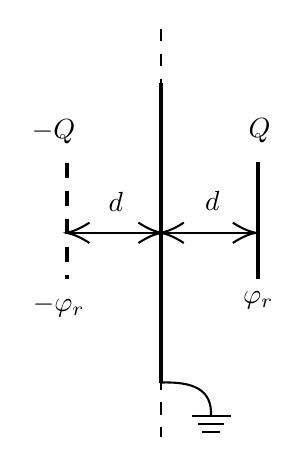
\begin{tikzpicture}[x=0.75pt,y=0.75pt,yscale=-1,xscale=1]
%uncomment if require: \path (0,214); %set diagram left start at 0, and has height of 214

%Straight Lines [id:da6610196299471309] 
\draw [line width=1.5]    (332,32.72) -- (332,177) ;
%Straight Lines [id:da44337749384706737] 
\draw    (346.65,193.14) -- (365.65,193.14) ;
%Straight Lines [id:da8821930896375005] 
\draw    (349.65,197.14) -- (362.4,197.14) ;
%Straight Lines [id:da2145551027408219] 
\draw    (351.69,200.64) -- (360.44,200.64) ;
%Straight Lines [id:da7689318007396346] 
\draw [line width=0.75]  [dash pattern={on 4.5pt off 4.5pt}]  (332,6.53) -- (332,203.2) ;
%Curve Lines [id:da21798502416376686] 
\draw    (332,177) .. controls (347.48,176.51) and (356.63,180.27) .. (356.06,193.13) ;
%Straight Lines [id:da7908665289748686] 
\draw [line width=1.5]    (378.62,70.85) -- (378.62,127.03) ;
%Straight Lines [id:da20723349218984932] 
\draw [line width=1.5]  [dash pattern={on 5.63pt off 4.5pt}]  (286.62,71.05) -- (286.62,127.23) ;
%Straight Lines [id:da4387491156358345] 
\draw    (288.52,104.86) -- (330,104.86) ;
\draw [shift={(332,104.86)}, rotate = 180] [color={rgb, 255:red, 0; green, 0; blue, 0 }  ][line width=0.75]    (10.93,-4.9) .. controls (6.95,-2.3) and (3.31,-0.67) .. (0,0) .. controls (3.31,0.67) and (6.95,2.3) .. (10.93,4.9)   ;
\draw [shift={(286.52,104.86)}, rotate = 0] [color={rgb, 255:red, 0; green, 0; blue, 0 }  ][line width=0.75]    (10.93,-4.9) .. controls (6.95,-2.3) and (3.31,-0.67) .. (0,0) .. controls (3.31,0.67) and (6.95,2.3) .. (10.93,4.9)   ;
%Straight Lines [id:da3047339949377774] 
\draw    (334,104.86) -- (375.48,104.86) ;
\draw [shift={(377.48,104.86)}, rotate = 180] [color={rgb, 255:red, 0; green, 0; blue, 0 }  ][line width=0.75]    (10.93,-4.9) .. controls (6.95,-2.3) and (3.31,-0.67) .. (0,0) .. controls (3.31,0.67) and (6.95,2.3) .. (10.93,4.9)   ;
\draw [shift={(332,104.86)}, rotate = 0] [color={rgb, 255:red, 0; green, 0; blue, 0 }  ][line width=0.75]    (10.93,-4.9) .. controls (6.95,-2.3) and (3.31,-0.67) .. (0,0) .. controls (3.31,0.67) and (6.95,2.3) .. (10.93,4.9)   ;

% Text Node
\draw (370,131.73) node [anchor=north west][inner sep=0.75pt]    {$\varphi_{r}$};
% Text Node
\draw (268.67,133.4) node [anchor=north west][inner sep=0.75pt]    {$-\varphi_{r}$};
% Text Node
\draw (372.67,48.4) node [anchor=north west][inner sep=0.75pt]    {$Q$};
% Text Node
\draw (305.22,83.88) node [anchor=north west][inner sep=0.75pt]    {$d$};
% Text Node
\draw (268.22,48.88) node [anchor=north west][inner sep=0.75pt]    {$-Q$};
% Text Node
\draw (351.72,83.38) node [anchor=north west][inner sep=0.75pt]    {$d$};


\end{tikzpicture}

    \end{minipage}
     Những bài toán như thế này thường được giải bằng phương pháp ảnh điện. Chúng ta lấy mặt phẳng vô hạn nối đất làm mặt phẳng đối xứng. Nếu các điện tích ảnh được lấy đối xứng với các điện tích thật qua mặt phẳng này và điện tích của các điện tích ảnh có độ lớn bằng các điện tích thật nhưng trái dấu, thì điện trường bên phải sẽ giống với điện trường cần phải tìm ở trên. Có lẽ cần chú ý rằng khi ta thêm vào các điện tích ảnh thì nói chung sự phân bố điện tích của hệ là không đối xứng. Nhưng phương trình Poisson (\ref{c181}) thì tuyến tính, do đó, điện thế $\varphi$ cũng không đối xứng giống như phân bố điện tích $\rho$.\\
    Trong bài toán của chúng ta, sử dụng phương pháp ảnh điện, ta nhận thấy rằng hệ mặt phẳng vô hạn và tấm phẳng hình vuông đặt cách nhau một khoảng $d$ giống như là hai tấm phẳng hình vuông có cùng kích thước đặt cách nhau $2d$, một tấm có điện thế $\varphi_r$ và điện tích $Q$, tấm còn lại có điện thế $-\varphi_r$ và điện tích $-Q$. Hai tấm phẳng này tạo thành một tụ điện. Bởi vì khoảng cách giữa hai tấm $2d$ là rất bé so với kích thước tấm phẳng $\sqrt{S}$, ta có thể ước tính điện dung hệ này 
    $$C'=\dfrac{\varepsilon_0S}{2d}.$$
    Tuy nhiên hiệu điện thế giữa hai bản tụ của hệ này là $2\varphi_r$, gấp đôi hiệu điện thế giữa hai bản tụ của hệ ban đầu gồm một tấm phẳng và một mặt phẳng vô hạn là $\varphi_r$, vậy nên điện dung của hệ ban đầu là $C=2C'=4,8\dv{pF}$.
    \end{loigiai}
    
    
\begin{vd}[Điện tích bị kẹp]
    Một điện tích điểm $+ q$ được đặt cách một tấm phẳng vô hạn dẫn điện một khoảng $a$. Lực tác dụng lên điện tích lúc này là $F_0$. Sau đó, một tấm phẳng vô hạn dẫn điện khác được đặt cách điện tích một khoảng $3a$ sao cho nó song song với tấm phẳng ban đầu và điện tích nằm ở giữa hai tấm. Lực tác dụng lên điện tích lúc này là $F'$. Tìm giá trị của $\displaystyle\dfrac{F'}{F_0}$ chính xác đến hàng phần trăm.
    \end{vd}
    \begin{loigiai}\\
    \textbf{Xét khi chỉ có một tấm phẳng.}\\
    Lực điện tác dụng lên điện tích
    $$F=\dfrac{q^2}{4\pi\varepsilon_0\tron{2a}^2}.$$
    \textbf{Xét khi có hai tấm.}\\ 
    Có hai hệ vô hạn các điện tích ảnh như hình vẽ.
    \begin{center}
\tikzset{every picture/.style={line width=0.75pt}} %set default line width to 0.75pt        

\begin{tikzpicture}[x=0.75pt,y=0.75pt,yscale=-1,xscale=1]
%uncomment if require: \path (0,200); %set diagram left start at 0, and has height of 200

%Straight Lines [id:da8267611848173362] 
\draw    (310.33,28.43) -- (310.33,181.33) ;
%Straight Lines [id:da3722801231427568] 
\draw    (390.33,28.43) -- (390.33,181.33) ;
%Shape: Circle [id:dp5028859142785822] 
\draw  [fill={rgb, 255:red, 0; green, 0; blue, 0 }  ,fill opacity=1 ] (366.5,96.53) .. controls (366.5,94.4) and (368.23,92.67) .. (370.37,92.67) .. controls (372.5,92.67) and (374.23,94.4) .. (374.23,96.53) .. controls (374.23,98.67) and (372.5,100.4) .. (370.37,100.4) .. controls (368.23,100.4) and (366.5,98.67) .. (366.5,96.53) -- cycle ;
%Shape: Circle [id:dp722755410760223] 
\draw  [fill={rgb, 255:red, 0; green, 0; blue, 0 }  ,fill opacity=1 ] (406.5,96.53) .. controls (406.5,94.4) and (408.23,92.67) .. (410.37,92.67) .. controls (412.5,92.67) and (414.23,94.4) .. (414.23,96.53) .. controls (414.23,98.67) and (412.5,100.4) .. (410.37,100.4) .. controls (408.23,100.4) and (406.5,98.67) .. (406.5,96.53) -- cycle ;
%Shape: Circle [id:dp5697330344682447] 
\draw  [fill={rgb, 255:red, 0; green, 0; blue, 0 }  ,fill opacity=1 ] (207.5,96.53) .. controls (207.5,94.4) and (209.23,92.67) .. (211.37,92.67) .. controls (213.5,92.67) and (215.23,94.4) .. (215.23,96.53) .. controls (215.23,98.67) and (213.5,100.4) .. (211.37,100.4) .. controls (209.23,100.4) and (207.5,98.67) .. (207.5,96.53) -- cycle ;
%Shape: Circle [id:dp415186379944654] 
\draw  [fill={rgb, 255:red, 0; green, 0; blue, 0 }  ,fill opacity=1 ] (540.5,96.53) .. controls (540.5,94.4) and (542.23,92.67) .. (544.37,92.67) .. controls (546.5,92.67) and (548.23,94.4) .. (548.23,96.53) .. controls (548.23,98.67) and (546.5,100.4) .. (544.37,100.4) .. controls (542.23,100.4) and (540.5,98.67) .. (540.5,96.53) -- cycle ;
%Straight Lines [id:da7176834375498908] 
\draw  [dash pattern={on 4.5pt off 4.5pt}]  (198.57,96.53) -- (566.57,96.53) ;
%Shape: Circle [id:dp7076071291278667] 
\draw   (198.68,42.09) .. controls (198.68,35.83) and (203.75,30.76) .. (210,30.76) .. controls (216.25,30.76) and (221.32,35.83) .. (221.32,42.09) .. controls (221.32,48.34) and (216.25,53.41) .. (210,53.41) .. controls (203.75,53.41) and (198.68,48.34) .. (198.68,42.09) -- cycle ;

% Text Node
\draw (204.83,99.93) node [anchor=north west][inner sep=0.75pt]    {$q$};
% Text Node
\draw (394.23,105.4) node [anchor=north west][inner sep=0.75pt]    {$-q$};
% Text Node
\draw (364.9,105.73) node [anchor=north west][inner sep=0.75pt]    {$q$};
% Text Node
\draw (525.56,103.4) node [anchor=north west][inner sep=0.75pt]    {$-q$};
% Text Node
\draw (373.73,77.23) node [anchor=north west][inner sep=0.75pt]    {$a$};
% Text Node
\draw (324.23,77.73) node [anchor=north west][inner sep=0.75pt]    {$3a$};
% Text Node
\draw (204.28,34.65) node [anchor=north west][inner sep=0.75pt]    {$1$};


\end{tikzpicture}

    \end{center}
    \begin{center}
        

\tikzset{every picture/.style={line width=0.75pt}} %set default line width to 0.75pt        

\begin{tikzpicture}[x=0.75pt,y=0.75pt,yscale=-1,xscale=1]
%uncomment if require: \path (0,200); %set diagram left start at 0, and has height of 200

%Straight Lines [id:da8267611848173362] 
\draw    (321.33,29.43) -- (321.33,182.33) ;
%Straight Lines [id:da3722801231427568] 
\draw    (401.33,29.43) -- (401.33,182.33) ;
%Shape: Circle [id:dp5028859142785822] 
\draw  [fill={rgb, 255:red, 0; green, 0; blue, 0 }  ,fill opacity=1 ] (377.5,97.53) .. controls (377.5,95.4) and (379.23,93.67) .. (381.37,93.67) .. controls (383.5,93.67) and (385.23,95.4) .. (385.23,97.53) .. controls (385.23,99.67) and (383.5,101.4) .. (381.37,101.4) .. controls (379.23,101.4) and (377.5,99.67) .. (377.5,97.53) -- cycle ;
%Shape: Circle [id:dp722755410760223] 
\draw  [fill={rgb, 255:red, 0; green, 0; blue, 0 }  ,fill opacity=1 ] (522.5,97.53) .. controls (522.5,95.4) and (524.23,93.67) .. (526.37,93.67) .. controls (528.5,93.67) and (530.23,95.4) .. (530.23,97.53) .. controls (530.23,99.67) and (528.5,101.4) .. (526.37,101.4) .. controls (524.23,101.4) and (522.5,99.67) .. (522.5,97.53) -- cycle ;
%Shape: Circle [id:dp5697330344682447] 
\draw  [fill={rgb, 255:red, 0; green, 0; blue, 0 }  ,fill opacity=1 ] (262.5,97.53) .. controls (262.5,95.4) and (264.23,93.67) .. (266.37,93.67) .. controls (268.5,93.67) and (270.23,95.4) .. (270.23,97.53) .. controls (270.23,99.67) and (268.5,101.4) .. (266.37,101.4) .. controls (264.23,101.4) and (262.5,99.67) .. (262.5,97.53) -- cycle ;
%Shape: Circle [id:dp415186379944654] 
\draw  [fill={rgb, 255:red, 0; green, 0; blue, 0 }  ,fill opacity=1 ] (171.5,97.53) .. controls (171.5,95.4) and (173.23,93.67) .. (175.37,93.67) .. controls (177.5,93.67) and (179.23,95.4) .. (179.23,97.53) .. controls (179.23,99.67) and (177.5,101.4) .. (175.37,101.4) .. controls (173.23,101.4) and (171.5,99.67) .. (171.5,97.53) -- cycle ;
%Straight Lines [id:da7176834375498908] 
\draw  [dash pattern={on 4.5pt off 4.5pt}]  (166.33,97.88) -- (558.69,97.88) ;
%Shape: Circle [id:dp7076071291278667] 
\draw   (164.68,36.09) .. controls (164.68,29.83) and (169.75,24.76) .. (176,24.76) .. controls (182.25,24.76) and (187.32,29.83) .. (187.32,36.09) .. controls (187.32,42.34) and (182.25,47.41) .. (176,47.41) .. controls (169.75,47.41) and (164.68,42.34) .. (164.68,36.09) -- cycle ;

% Text Node
\draw (521.83,103.93) node [anchor=north west][inner sep=0.75pt]    {$q$};
% Text Node
\draw (252.73,102.4) node [anchor=north west][inner sep=0.75pt]    {$-q$};
% Text Node
\draw (375.9,106.73) node [anchor=north west][inner sep=0.75pt]    {$q$};
% Text Node
\draw (158.56,101.4) node [anchor=north west][inner sep=0.75pt]    {$-q$};
% Text Node
\draw (384.73,78.23) node [anchor=north west][inner sep=0.75pt]    {$a$};
% Text Node
\draw (335.23,78.73) node [anchor=north west][inner sep=0.75pt]    {$3a$};
% Text Node
\draw (170.28,28.65) node [anchor=north west][inner sep=0.75pt]    {$2$};


\end{tikzpicture}

    \end{center}
    Với hệ thứ nhất, khoảng cách từ các điện tích ảnh đến $q$ như sau.
    \begin{equation*}
        \begin{aligned}
            d_1&=(1+1)a=2a\\
            d_2&=(1+4+3)a=8a\\
            d_3&=(1+4+4+1)a=10a\\
            d_4&=(1+4+4+4+3)=12a\\
            ...
        \end{aligned}
    \end{equation*}
    Lực điện tác dụng lên điện tích $q$ do hệ điện tích ảnh này là
    \begin{equation*}
    \begin{aligned}
         F_+&=\dfrac{q^2}{4\pi\varepsilon_0}\tron{\dfrac{1}{{d_1}^2}+\dfrac{1}{{d_2}^2}+\dfrac{1}{{d_3}^2}+\dfrac{1}{{d_4}^2}+...}\\
        &=\dfrac{q^2}{4\pi\varepsilon_0a^2}\tron{\sum_{k=0}^\infty\tron{\dfrac{1}{\tron{2+4(2k)}^2}+\dfrac{1}{(4+4(2k+1))^2}}}.
    \end{aligned}
    \end{equation*}
    Với hệ điện tích ảnh thứ hai, khoảng cách từ các điện tích tới $q$ như sau.
    \begin{equation*}
        \begin{aligned}
            d'_1&=(3+3)a=6a\\
            d'_2&=(3+4+1)a=8a\\
            d'_3&=(3+4+4+3)a=14a\\
            d'_4&=(3+4+4+4+1)=12a\\
            ... 
        \end{aligned}
    \end{equation*}
    Lực điện do hệ điện tích ảnh tác dụng lên $q$ là
    \begin{equation*}
    \begin{aligned}
         F_-&=-\dfrac{q^2}{4\pi\varepsilon_0}\tron{\dfrac{1}{{d'_1}^2}+\dfrac{1}{{d'_2}^2}+\dfrac{1}{{d'_3}^2}+\dfrac{1}{{d'_4}^2}+...}\\
        &=-\dfrac{q^2}{4\pi\varepsilon_0a^2}\tron{\sum_{k=0}^\infty\tron{\dfrac{1}{\tron{6+4(2k)}^2}+\dfrac{1}{(4+4(2k+1))^2}}}.
    \end{aligned}
    \end{equation*}
    Hợp lực tác dụng lên điện tích
    \begin{equation*}
        \begin{aligned}
            F'&=F_++F_-\\
            &=\dfrac{q^2}{4\pi\varepsilon_0a^2}\tron{\sum_{k=0}^\infty\tron{\dfrac{1}{\tron{2+4(2k)}^2}-\dfrac{1}{\tron{6+4(2k)}^2}}}\\
            &=\dfrac{q^2}{16\pi\varepsilon_0a^2}\tron{\sum_{k=0}^\infty\tron{\dfrac{1}{\tron{1+4k}^2}-\dfrac{1}{\tron{3+4k}^2}}}\\
            &=\dfrac{q^2}{16\pi\varepsilon_0a^2}\tron{\dfrac{1}{1^2}-\dfrac{1}{3^2}+\dfrac{1}{5^2}-\dfrac{1}{7^2}+...}.
        \end{aligned}
    \end{equation*}
    Giá trị $G=\dfrac{1}{1^2}-\dfrac{1}{3^2}+\dfrac{1}{5^2}-\dfrac{1}{7^2}+...$  là hằng số Catalan và $G\approx0.916$. Đề bài chỉ yêu cầu ta tính chính xác đến hàng phần trăm nên ta có thể bấm máy
    $$\dfrac{F'}{F}=G\approx\dfrac{1}{1^2}-\dfrac{1}{3^2}+\dfrac{1}{5^2}-\dfrac{1}{7^2}+\dfrac{1}{9^2}-\dfrac{1}{11^2}\approx0.91$$.
    \end{loigiai}
    
    
    \begin{vd}[Điện tích và quả cầu nối đất]
Một điện tích điểm mang điện tích dương $q$ được đặt gần một quả cầu kim loại bán kính $R$. Quả cầu được nối đất và giữ cố định. 
 \begin{enumerate}[1)]
     \item Điện tích điểm $q$ được đặt cố định tại một điểm nằm cách tâm quả cầu một khoảng $d$ (Hình vẽ). Xác định véctơ cường độ điện trường $\ot{E}$ tại các điểm nằm trên đường nối điện tích và tâm quả cầu, cách điện tích $q$ một khoảng $r$. Vẽ phác dạng đồ thị về sự phụ thuộc cường độ điện trường $E$ theo khoảng cách $r$.
     \begin{center}
         

\tikzset{every picture/.style={line width=0.75pt}} %set default line width to 0.75pt        

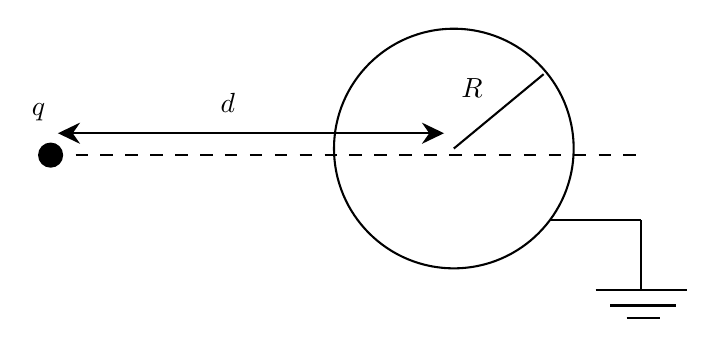
\begin{tikzpicture}[x=0.75pt,y=0.75pt,yscale=-1,xscale=1]
%uncomment if require: \path (0,300); %set diagram left start at 0, and has height of 300

%Shape: Circle [id:dp5933878184777908] 
\draw   (276.09,204.36) .. controls (276.09,172.48) and (301.94,146.64) .. (333.82,146.64) .. controls (365.7,146.64) and (391.55,172.48) .. (391.55,204.36) .. controls (391.55,236.25) and (365.7,262.09) .. (333.82,262.09) .. controls (301.94,262.09) and (276.09,236.25) .. (276.09,204.36) -- cycle ;
%Straight Lines [id:da726936917517762] 
\draw    (146.09,197) -- (326.09,197) ;
\draw [shift={(329.09,197)}, rotate = 180] [fill={rgb, 255:red, 0; green, 0; blue, 0 }  ][line width=0.08]  [draw opacity=0] (10.72,-5.15) -- (0,0) -- (10.72,5.15) -- (7.12,0) -- cycle    ;
\draw [shift={(143.09,197)}, rotate = 0] [fill={rgb, 255:red, 0; green, 0; blue, 0 }  ][line width=0.08]  [draw opacity=0] (10.72,-5.15) -- (0,0) -- (10.72,5.15) -- (7.12,0) -- cycle    ;
%Shape: Circle [id:dp25683169640140746] 
\draw  [fill={rgb, 255:red, 0; green, 0; blue, 0 }  ,fill opacity=1 ] (134,207.55) .. controls (134,204.48) and (136.48,202) .. (139.55,202) .. controls (142.61,202) and (145.09,204.48) .. (145.09,207.55) .. controls (145.09,210.61) and (142.61,213.09) .. (139.55,213.09) .. controls (136.48,213.09) and (134,210.61) .. (134,207.55) -- cycle ;
%Straight Lines [id:da5559809757169798] 
\draw  [dash pattern={on 4.5pt off 4.5pt}]  (139.55,207.55) -- (422.09,207.55) ;
%Straight Lines [id:da928704635393939] 
\draw    (377.09,168.55) -- (333.82,204.36) ;
%Straight Lines [id:da4790198920717281] 
\draw    (380.09,239) -- (424.09,239) ;
%Straight Lines [id:da1289355410830988] 
\draw    (424.09,239) -- (424.09,272.55) ;
%Straight Lines [id:da5769846178982978] 
\draw    (402.09,272.55) -- (446.09,272.55) ;
%Straight Lines [id:da8295141937851105] 
\draw    (409.09,280) -- (441.09,280) ;
%Straight Lines [id:da4483775147940956] 
\draw    (417.09,286) -- (433.09,286) ;


% Text Node
\draw (336,169.4) node [anchor=north west][inner sep=0.75pt]    {$R$};
% Text Node
\draw (220,176.4) node [anchor=north west][inner sep=0.75pt]    {$d$};
% Text Node
\draw (129,181.4) node [anchor=north west][inner sep=0.75pt]    {$q$};


\end{tikzpicture}

     \end{center}
     \item Điện tích điểm $q$ có khối lượng $m$ được nối với một sợi dây mềm, nhẹ, mảnh, không dãn, cách điện và có chiều dài $\ell .$ Đầu kia của dây được gắn vào điểm O cố định (Hình vẽ). Điểm O và tâm quả cầu cách nhau $L$ $(L>\ell +R)$. Bỏ qua tác dụng của trọng lực. Kích thích để $q$ dao động nhỏ trong điện trường. Tìm tần số dao động.
     \begin{center}
         

\tikzset{every picture/.style={line width=0.75pt}} %set default line width to 0.75pt        

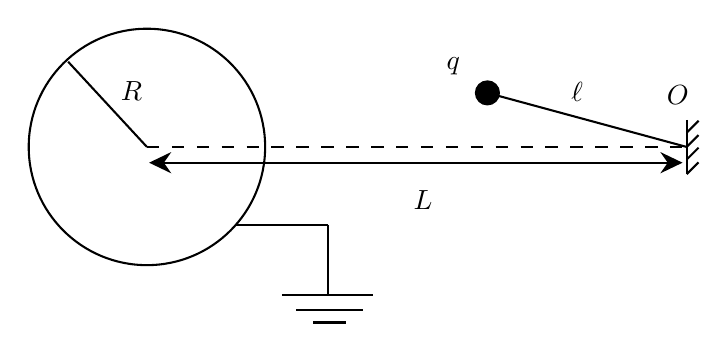
\begin{tikzpicture}[x=0.75pt,y=0.75pt,yscale=-1,xscale=1]
%uncomment if require: \path (0,607); %set diagram left start at 0, and has height of 607

%Shape: Circle [id:dp030408007945189608] 
\draw   (109.09,385.41) .. controls (109.09,353.95) and (134.59,328.45) .. (166.05,328.45) .. controls (197.5,328.45) and (223,353.95) .. (223,385.41) .. controls (223,416.86) and (197.5,442.36) .. (166.05,442.36) .. controls (134.59,442.36) and (109.09,416.86) .. (109.09,385.41) -- cycle ;
%Straight Lines [id:da9843302544726922] 
\draw  [dash pattern={on 4.5pt off 4.5pt}]  (166.05,385.41) -- (426.09,385.41) ;
%Straight Lines [id:da6534329890285495] 
\draw    (166.05,385.41) -- (128.09,344.36) ;
%Straight Lines [id:da4299218767169213] 
\draw    (170.09,393) -- (251.09,393) -- (421.09,393) ;
\draw [shift={(424.09,393)}, rotate = 180] [fill={rgb, 255:red, 0; green, 0; blue, 0 }  ][line width=0.08]  [draw opacity=0] (10.72,-5.15) -- (0,0) -- (10.72,5.15) -- (7.12,0) -- cycle    ;
\draw [shift={(167.09,393)}, rotate = 0] [fill={rgb, 255:red, 0; green, 0; blue, 0 }  ][line width=0.08]  [draw opacity=0] (10.72,-5.15) -- (0,0) -- (10.72,5.15) -- (7.12,0) -- cycle    ;
%Straight Lines [id:da4433401200906899] 
\draw    (426.09,385.41) -- (330.09,359.36) ;
%Shape: Circle [id:dp45916852044082535] 
\draw  [fill={rgb, 255:red, 0; green, 0; blue, 0 }  ,fill opacity=1 ] (324.55,359.36) .. controls (324.55,356.3) and (327.03,353.82) .. (330.09,353.82) .. controls (333.15,353.82) and (335.64,356.3) .. (335.64,359.36) .. controls (335.64,362.43) and (333.15,364.91) .. (330.09,364.91) .. controls (327.03,364.91) and (324.55,362.43) .. (324.55,359.36) -- cycle ;
%Straight Lines [id:da5755357704056867] 
\draw    (209.09,423) -- (253.09,423) ;
%Straight Lines [id:da6932620392012379] 
\draw    (253.09,423) -- (253.09,456.55) ;
%Straight Lines [id:da4870726310747] 
\draw    (231.09,456.55) -- (275.09,456.55) ;
%Straight Lines [id:da03929075961019057] 
\draw    (238.09,464) -- (270.09,464) ;
%Straight Lines [id:da18688277593452685] 
\draw    (246.09,470) -- (262.09,470) ;
%Straight Lines [id:da7391045314725575] 
\draw    (426.09,372.31) -- (426.09,398.51) ;
%Straight Lines [id:da699700317404319] 
\draw    (431.8,372.8) -- (426.09,378.51) ;
%Straight Lines [id:da8368994959800724] 
\draw    (431.8,379.7) -- (426.09,385.41) ;
%Straight Lines [id:da25171942248153245] 
\draw    (431.8,385.8) -- (426.09,391.51) ;
%Straight Lines [id:da9383187021800725] 
\draw    (431.8,392.8) -- (426.09,398.51) ;

% Text Node
\draw (152,352.4) node [anchor=north west][inner sep=0.75pt]    {$R$};
% Text Node
\draw (309,340.76) node [anchor=north west][inner sep=0.75pt]    {$q$};
% Text Node
\draw (369,352.76) node [anchor=north west][inner sep=0.75pt]    {$\ell $};
% Text Node
\draw (293,404.76) node [anchor=north west][inner sep=0.75pt]    {$L$};
% Text Node
\draw (415,354.4) node [anchor=north west][inner sep=0.75pt]    {$O$};


\end{tikzpicture}

     \end{center}
 \end{enumerate}
 
\end{vd}

\begin{loigiai}
    \begin{enumerate}[1)]
        \item Dùng phương pháp ảnh điện, xác định điện tích $q'$ tương đương với điện tích trên mặt quả cầu:
        Điện tích $q'$ nằm trên đường thẳng nối tâm quả cầu và điện tích $q$, cách tâm quả cầu một đoạn $d'$. Do quả cầu nối đất, điện thế tại một điểm B bất kỳ trên mặt cầu bằng $0$. B cách $q$, $q'$ lần lượt là $r_1$, $r_2$. Ta có:
    \[{{V}_{B}}=\dfrac{1}{4\pi {{\varepsilon }_{0}}}\left( \dfrac{q}{{{r}_{1}}}+\dfrac{q'}{{{r}_{2}}} \right)=0 \,\,\,\,\Rightarrow \dfrac{q}{{{r}_{1}}}+\dfrac{q'}{{{r}_{2}}}=0 \tag{1} \label{tr.tst.3.1} \]
    Trong đó: 
    \[\heva{{r_1}=\sqrt{{{R}^{2}}+{{d}^{2}}-2Rd\cos \alpha }\\
        {r_2} = \sqrt {{R^2} + d{'^2} - 2Rd'\cos \alpha }} \tag{2} \label{tr.tst.3.2}\]
    Từ (\ref{tr.tst.3.1}) và (\ref{tr.tst.3.2}):
    \[q'=-q\dfrac{R}{d},\]
    \[d'=\dfrac{R^2}{d}.\]
    Ta đi xét điện trường tổng hợp tạo ra bởi điện tích $q$ và ảnh điện $q'$.
    \begin{center}
        

\tikzset{every picture/.style={line width=0.75pt}} %set default line width to 0.75pt        

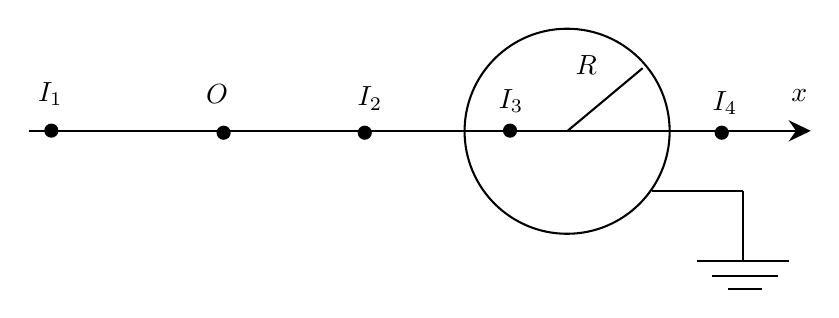
\begin{tikzpicture}[x=0.75pt,y=0.75pt,yscale=-1,xscale=1]
%uncomment if require: \path (0,300); %set diagram left start at 0, and has height of 300

%Shape: Circle [id:dp7591737796642399] 
\draw   (302,142.2) .. controls (302,114.92) and (324.12,92.8) .. (351.4,92.8) .. controls (378.68,92.8) and (400.8,114.92) .. (400.8,142.2) .. controls (400.8,169.48) and (378.68,191.6) .. (351.4,191.6) .. controls (324.12,191.6) and (302,169.48) .. (302,142.2) -- cycle ;
%Straight Lines [id:da2795044321465334] 
\draw    (92,142) -- (465.8,142) ;
\draw [shift={(468.8,142)}, rotate = 180] [fill={rgb, 255:red, 0; green, 0; blue, 0 }  ][line width=0.08]  [draw opacity=0] (10.72,-5.15) -- (0,0) -- (10.72,5.15) -- (7.12,0) -- cycle    ;
%Shape: Circle [id:dp5960660117037158] 
\draw  [fill={rgb, 255:red, 0; green, 0; blue, 0 }  ,fill opacity=1 ] (100,141.9) .. controls (100,140.3) and (101.3,139) .. (102.9,139) .. controls (104.5,139) and (105.8,140.3) .. (105.8,141.9) .. controls (105.8,143.5) and (104.5,144.8) .. (102.9,144.8) .. controls (101.3,144.8) and (100,143.5) .. (100,141.9) -- cycle ;
%Shape: Circle [id:dp19140326226977633] 
\draw  [fill={rgb, 255:red, 0; green, 0; blue, 0 }  ,fill opacity=1 ] (183,142.9) .. controls (183,141.3) and (184.3,140) .. (185.9,140) .. controls (187.5,140) and (188.8,141.3) .. (188.8,142.9) .. controls (188.8,144.5) and (187.5,145.8) .. (185.9,145.8) .. controls (184.3,145.8) and (183,144.5) .. (183,142.9) -- cycle ;
%Shape: Circle [id:dp2892500024246949] 
\draw  [fill={rgb, 255:red, 0; green, 0; blue, 0 }  ,fill opacity=1 ] (251,142.9) .. controls (251,141.3) and (252.3,140) .. (253.9,140) .. controls (255.5,140) and (256.8,141.3) .. (256.8,142.9) .. controls (256.8,144.5) and (255.5,145.8) .. (253.9,145.8) .. controls (252.3,145.8) and (251,144.5) .. (251,142.9) -- cycle ;
%Shape: Circle [id:dp3885538696995159] 
\draw  [fill={rgb, 255:red, 0; green, 0; blue, 0 }  ,fill opacity=1 ] (321,141.9) .. controls (321,140.3) and (322.3,139) .. (323.9,139) .. controls (325.5,139) and (326.8,140.3) .. (326.8,141.9) .. controls (326.8,143.5) and (325.5,144.8) .. (323.9,144.8) .. controls (322.3,144.8) and (321,143.5) .. (321,141.9) -- cycle ;
%Shape: Circle [id:dp7968960876850744] 
\draw  [fill={rgb, 255:red, 0; green, 0; blue, 0 }  ,fill opacity=1 ] (423,142.9) .. controls (423,141.3) and (424.3,140) .. (425.9,140) .. controls (427.5,140) and (428.8,141.3) .. (428.8,142.9) .. controls (428.8,144.5) and (427.5,145.8) .. (425.9,145.8) .. controls (424.3,145.8) and (423,144.5) .. (423,142.9) -- cycle ;
%Straight Lines [id:da680401206641736] 
\draw    (351.4,142.2) -- (387.8,111.8) ;
%Straight Lines [id:da5514526288105313] 
\draw    (392.09,171) -- (436.09,171) ;
%Straight Lines [id:da8750775768425993] 
\draw    (436.09,171) -- (436.09,204.55) ;
%Straight Lines [id:da7918333595649452] 
\draw    (414.09,204.55) -- (458.09,204.55) ;
%Straight Lines [id:da8289334767112873] 
\draw    (421.09,212) -- (453.09,212) ;
%Straight Lines [id:da2559534753805328] 
\draw    (429.09,218) -- (445.09,218) ;


% Text Node
\draw (95,117.2) node [anchor=north west][inner sep=0.75pt]    {$I_{1}$};
% Text Node
\draw (176,118.4) node [anchor=north west][inner sep=0.75pt]    {$O$};
% Text Node
\draw (249,119.4) node [anchor=north west][inner sep=0.75pt]    {$I_{2}$};
% Text Node
\draw (317,120.4) node [anchor=north west][inner sep=0.75pt]    {$I_{3}$};
% Text Node
\draw (354,104.4) node [anchor=north west][inner sep=0.75pt]    {$R$};
% Text Node
\draw (420,121.4) node [anchor=north west][inner sep=0.75pt]    {$I_{4}$};
% Text Node
\draw (458,120.4) node [anchor=north west][inner sep=0.75pt]    {$x$};


\end{tikzpicture}

    \end{center}
    Tại các điểm nằm ngoài quả cầu trên đường nối điện tích và tâm quả cầu, cách điện tích một khoảng $r>0$:
    \[{\ot{E_{{I}_{1}}}}=\dfrac{1}{4\pi {{\varepsilon }_{0}}}\left[ \dfrac{q}{{{r}^{2}}}-\dfrac{q\dfrac{R}{d}}{{{\left( r+d-\dfrac{{{R}^{2}}}{d} \right)}^{2}}} \right]\dfrac{{\ot{r}}}{r};\]
    \[{{\ot{E_{{I}_{2}}}}}=\dfrac{1}{4\pi {{\varepsilon }_{0}}}\left[ \dfrac{q}{{{r}^{2}}}+\dfrac{q\dfrac{R}{d}}{{{\left( -r+d-\dfrac{{{R}^{2}}}{d} \right)}^{2}}} \right]\dfrac{{\ot{r}}}{r};\]
    \[{{{E_{{I}_{4}}}}}=\dfrac{1}{4\pi {{\varepsilon }_{0}}}\left[ \dfrac{q}{{{r}^{2}}}-\dfrac{q\dfrac{R}{d}}{{{\left( r-d+\dfrac{{{R}^{2}}}{d} \right)}^{2}}} \right]\dfrac{{\ot{r}}}{r}.\]
    Tại các điểm bên trong quả cầu: ${{\ot{E_{{I}_{3}}}}}=0$.
    Đồ thị $E(x)$ có dạng như hình vẽ:
    \begin{center}
        

\tikzset{every picture/.style={line width=0.75pt}} %set default line width to 0.75pt        

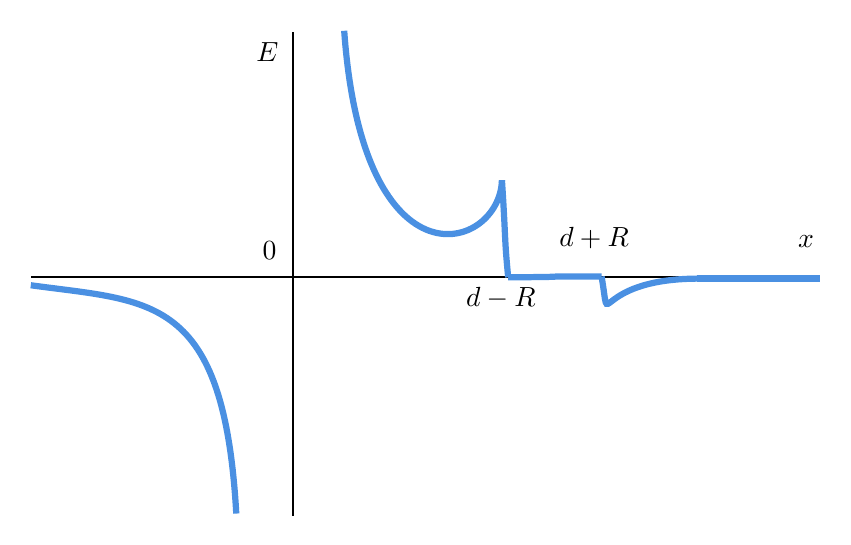
\begin{tikzpicture}[x=0.75pt,y=0.75pt,yscale=-1,xscale=1]
%uncomment if require: \path (0,300); %set diagram left start at 0, and has height of 300

%Straight Lines [id:da32567883731904246] 
\draw    (144,155) -- (523.8,155) ;
%Straight Lines [id:da01599842013690056] 
\draw    (270,37) -- (270,270) ;
%Curve Lines [id:da679532167825887] 
\draw [color={rgb, 255:red, 74; green, 144; blue, 226 }  ,draw opacity=1 ][line width=2.25]    (143.8,159) .. controls (201.8,167) and (236.8,163) .. (242.8,269) ;
%Curve Lines [id:da23563833057271877] 
\draw [color={rgb, 255:red, 74; green, 144; blue, 226 }  ,draw opacity=1 ][line width=2.25]    (294.8,36.4) .. controls (303.8,163.4) and (369.8,142.4) .. (370.8,108.4) ;
%Curve Lines [id:da31110618594065986] 
\draw [color={rgb, 255:red, 74; green, 144; blue, 226 }  ,draw opacity=1 ][line width=2.25]    (373.8,155.2) .. controls (371.8,134) and (372.8,139.2) .. (370.8,108.4) ;
%Curve Lines [id:da4120593954231564] 
\draw [color={rgb, 255:red, 74; green, 144; blue, 226 }  ,draw opacity=1 ][line width=2.25]    (418.8,154.8) .. controls (373.8,154.8) and (418.8,154.8) .. (373.8,155.2) ;
%Curve Lines [id:da9198661808119668] 
\draw [color={rgb, 255:red, 74; green, 144; blue, 226 }  ,draw opacity=1 ][line width=2.25]    (464.8,155.8) .. controls (412.8,156.2) and (423.8,183.8) .. (418.8,154.8) ;
%Straight Lines [id:da266849848588921] 
\draw [color={rgb, 255:red, 74; green, 144; blue, 226 }  ,draw opacity=1 ][line width=2.25]    (464.8,155.8) -- (523.8,155.8) ;


% Text Node
\draw (251,40.4) node [anchor=north west][inner sep=0.75pt]    {$E$};
% Text Node
\draw (254,136.4) node [anchor=north west][inner sep=0.75pt]    {$0$};
% Text Node
\draw (352,158.4) node [anchor=north west][inner sep=0.75pt]    {$d-R$};
% Text Node
\draw (397,129.4) node [anchor=north west][inner sep=0.75pt]    {$d+R$};
% Text Node
\draw (512,133.4) node [anchor=north west][inner sep=0.75pt]    {$x$};


\end{tikzpicture}

    \end{center}
    \item Khoảng cách từ điện tích q đến tâm quả cầu là:
    \[d=\sqrt{{{L}^{2}}+{{\ell }^{2}}-2L\ell \cos \alpha }. \tag{3} \label{tr.tst.3.3}\]
    Điện tích cảm ứng trên mặt cầu tương đương với điện tích $q'$ được xác định trong câu trước. Do đó lực điện tác dụng lên $q$ là: 	
    \[F=\dfrac{1}{4\pi {{\varepsilon }_{0}}}\dfrac{qq'}{{{\left( d-d' \right)}^{2}}}=\dfrac{1}{4\pi {{\varepsilon }_{0}}}\dfrac{{{q}^{2}}Rd}{{{\left( {{d}^{2}}-{{R}^{2}} \right)}^{2}}}. \tag{4} \label{tr.tst.3.4}\]
    Thay giá trị của $d$ từ (\ref{tr.tst.3.3}) vào (\ref{tr.tst.3.4}): 
    \[F=\dfrac{1}{4\pi {{\varepsilon }_{0}}}\dfrac{{{q}^{2}}R\sqrt{{{L}^{2}}+{{\ell }^{2}}-2L\ell \cos \alpha }}{{{\left( {{L}^{2}}+{{\ell }^{2}}-2L\ell \cos \alpha -{{R}^{2}} \right)}^{2}}}.\]
    Lực $\ot{F}$ là lực hút, có hướng dọc theo đường thẳng nối $q$ và $q'$. Lực làm điện tích $q$ dao động là thành phần hình chiếu ${{F}_{\bot }}$ của $\ot{F}$ lên phương vuông góc với dây treo.
	\[{{F}_{\bot }}=\dfrac{1}{4\pi {{\varepsilon }_{0}}}\dfrac{{{q}^{2}}R\sqrt{{{L}^{2}}+{{\ell }^{2}}-2L\ell \cos \alpha }}{{{\left( {{L}^{2}}+{{\ell }^{2}}-2L\ell \cos \alpha -{{R}^{2}} \right)}^{2}}}\sin \left( \alpha +\beta  \right),\]
	với $\ell \sin \alpha =d\sin \beta .$
    \begin{center}
\tikzset{every picture/.style={line width=0.75pt}} %set default line width to 0.75pt        

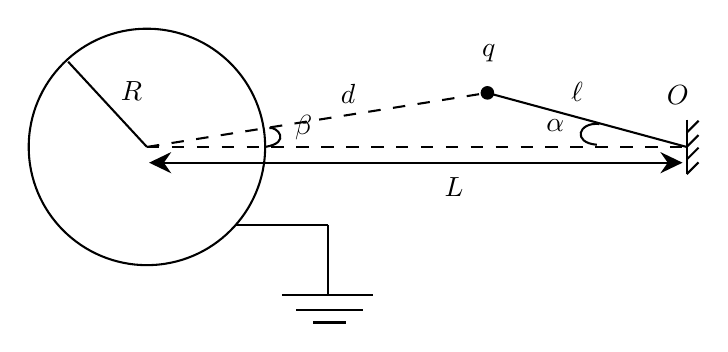
\begin{tikzpicture}[x=0.75pt,y=0.75pt,yscale=-1,xscale=1]
%uncomment if require: \path (0,300); %set diagram left start at 0, and has height of 300

%Shape: Circle [id:dp32399485336727984] 
\draw   (149.09,145.05) .. controls (149.09,113.59) and (174.59,88.09) .. (206.05,88.09) .. controls (237.5,88.09) and (263,113.59) .. (263,145.05) .. controls (263,176.5) and (237.5,202) .. (206.05,202) .. controls (174.59,202) and (149.09,176.5) .. (149.09,145.05) -- cycle ;
%Straight Lines [id:da24390951084419066] 
\draw  [dash pattern={on 4.5pt off 4.5pt}]  (206.05,145.05) -- (466.09,145.05) ;
%Straight Lines [id:da6082251030986507] 
\draw    (206.05,145.05) -- (168.09,104) ;
%Straight Lines [id:da8222526869413775] 
\draw    (210.09,152.64) -- (291.09,152.64) -- (461.09,152.64) ;
\draw [shift={(464.09,152.64)}, rotate = 180] [fill={rgb, 255:red, 0; green, 0; blue, 0 }  ][line width=0.08]  [draw opacity=0] (10.72,-5.15) -- (0,0) -- (10.72,5.15) -- (7.12,0) -- cycle    ;
\draw [shift={(207.09,152.64)}, rotate = 0] [fill={rgb, 255:red, 0; green, 0; blue, 0 }  ][line width=0.08]  [draw opacity=0] (10.72,-5.15) -- (0,0) -- (10.72,5.15) -- (7.12,0) -- cycle    ;
%Straight Lines [id:da15124326175328684] 
\draw    (466.09,145.05) -- (370.09,119) ;
%Shape: Circle [id:dp48130578547425706] 
\draw  [fill={rgb, 255:red, 0; green, 0; blue, 0 }  ,fill opacity=1 ] (367.32,119) .. controls (367.32,117.47) and (368.56,116.23) .. (370.09,116.23) .. controls (371.62,116.23) and (372.86,117.47) .. (372.86,119) .. controls (372.86,120.53) and (371.62,121.77) .. (370.09,121.77) .. controls (368.56,121.77) and (367.32,120.53) .. (367.32,119) -- cycle ;
%Straight Lines [id:da676344864372332] 
\draw    (249.09,182.64) -- (293.09,182.64) ;
%Straight Lines [id:da5101228153893618] 
\draw    (293.09,182.64) -- (293.09,216.18) ;
%Straight Lines [id:da11669328176512872] 
\draw    (271.09,216.18) -- (315.09,216.18) ;
%Straight Lines [id:da8805261245626324] 
\draw    (278.09,223.64) -- (310.09,223.64) ;
%Straight Lines [id:da9125584462465555] 
\draw    (286.09,229.64) -- (302.09,229.64) ;
%Straight Lines [id:da9788206752359616] 
\draw    (466.09,131.95) -- (466.09,158.15) ;
%Straight Lines [id:da7868788067689376] 
\draw    (471.8,132.44) -- (466.09,138.15) ;
%Straight Lines [id:da8920513204038671] 
\draw    (471.8,139.34) -- (466.09,145.05) ;
%Straight Lines [id:da5951887022015814] 
\draw    (471.8,145.44) -- (466.09,151.15) ;
%Straight Lines [id:da17105130468742602] 
\draw    (471.8,152.44) -- (466.09,158.15) ;
%Straight Lines [id:da5141540989489952] 
\draw  [dash pattern={on 4.5pt off 4.5pt}]  (206.05,145.05) -- (370.09,119) ;
%Curve Lines [id:da7828224153250147] 
\draw    (265,136) .. controls (268.8,135) and (275.8,143) .. (263,145.05) ;
%Curve Lines [id:da7754975024139585] 
\draw    (424,134) .. controls (413.8,133) and (410.8,143) .. (422.8,144) ;


% Text Node
\draw (192,112.04) node [anchor=north west][inner sep=0.75pt]    {$R$};
% Text Node
\draw (366,94.4) node [anchor=north west][inner sep=0.75pt]    {$q$};
% Text Node
\draw (409,112.4) node [anchor=north west][inner sep=0.75pt]    {$\ell $};
% Text Node
\draw (348,158.4) node [anchor=north west][inner sep=0.75pt]    {$L$};
% Text Node
\draw (455,114.04) node [anchor=north west][inner sep=0.75pt]    {$O$};
% Text Node
\draw (298,113.4) node [anchor=north west][inner sep=0.75pt]    {$d$};
% Text Node
\draw (276,128.4) node [anchor=north west][inner sep=0.75pt]    {$\beta $};
% Text Node
\draw (397,130.4) node [anchor=north west][inner sep=0.75pt]    {$\alpha $};


\end{tikzpicture}
\end{center}
    Áp dụng định luật II Newton: 
    \[m\ell \alpha ''=-{{F}_{\bot }}=-\dfrac{1}{4\pi {{\varepsilon }_{0}}}\dfrac{{{q}^{2}}R\sqrt{{{L}^{2}}+{{\ell }^{2}}-2L\ell \cos \alpha }}{{{\left( {{L}^{2}}+{{\ell }^{2}}-2L\ell \cos \alpha -{{R}^{2}} \right)}^{2}}}\sin \left( \alpha +\beta  \right).\]
    Với các dao động bé, ta được: 
	\[m\ell \alpha ''+\dfrac{1}{4\pi {{\varepsilon }_{0}}}\dfrac{{{q}^{2}}Rd}{{{\left( {{d}^{2}}-{{R}^{2}} \right)}^{2}}}\left( 1+\dfrac{\ell }{d} \right)\alpha =0,\]	
	với $\beta \approx \dfrac{\alpha \ell }{L-\ell }$.
	\\Từ đó ta tìm được tần số góc dao động bé của $q$ là: $\omega =\dfrac{q}{{{d}^{2}}-{{R}^{2}}}\sqrt{\dfrac{Rd}{4\pi {{\varepsilon }_{0}}}\dfrac{1}{m\ell }\left( 1+\dfrac{\ell }{d} \right)}$.
	\\Hay:
	$$\omega =\dfrac{q}{{{\left( L-\ell  \right)}^{2}}-{{R}^{2}}}\sqrt{\dfrac{RL}{4\pi {{\varepsilon }_{0}}}\dfrac{1}{m\ell }}.$$
	\end{enumerate}
\end{loigiai}


\begin{vd}[Thí nghiệm của Coulomb]
Trong thí nghiệm gốc của mình, Coulomb đã đo lực tương tác giữa hai vỏ cầu kim loại tích điện chứ không phải hai “điện tích” thuần túy. Chúng ta đã biết rằng điện trường gây ra bởi một mặt cầu tích điện đều là tương tự với điện trường của điện tích điểm và do đó lực tương tác giữa hai phân bố điện tích đối xứng cầu là tương đương với lực tương tác của hai điện tích điểm 
      $$\ot{F} = k_e \frac{q_1 q_2}{r^2} \hat{{r}}, $$ 
ở đây $q_1$ và $q_2$ là tổng điện tích trên 2 mặt cầu, và $\ot{r} = r\cdot\hat{{r}}$ là khoảng cách giữa hai tâm của các mặt cầu. Nhưng chúng ta cũng biết rằng điện trường hưởng ứng sẽ làm thay đổi phân bố điện tích bề mặt của vật dẫn do đó phương trình lực như đã nói cần thêm một phần bổ chính. Chúng ta dự đoán rằng hiện tượng hưởng ứng là đáng kể khi bán kính $a$ của quả cầu có thể so sánh được với cỡ của khoảng cách $r$.
\begin{center}


\tikzset{every picture/.style={line width=0.75pt}} %set default line width to 0.75pt        

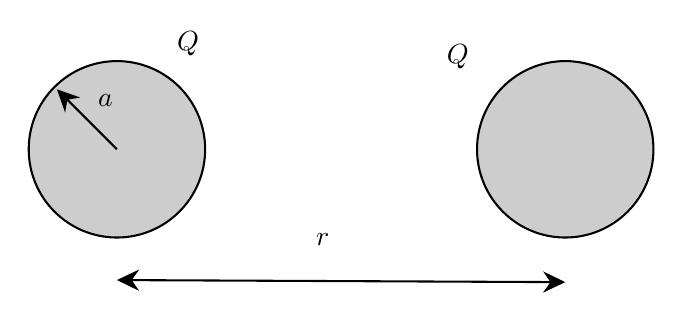
\begin{tikzpicture}[x=0.75pt,y=0.75pt,yscale=-1,xscale=1]
%uncomment if require: \path (0,300); %set diagram left start at 0, and has height of 300

%Shape: Circle [id:dp7981883866523323] 
\draw  [fill={rgb, 255:red, 155; green, 155; blue, 155 }  ,fill opacity=0.5 ] (110,108.5) .. controls (110,85.03) and (129.03,66) .. (152.5,66) .. controls (175.97,66) and (195,85.03) .. (195,108.5) .. controls (195,131.97) and (175.97,151) .. (152.5,151) .. controls (129.03,151) and (110,131.97) .. (110,108.5) -- cycle ;
%Straight Lines [id:da5117487151827391] 
\draw    (152.5,108.5) -- (125.72,81.72) ;
\draw [shift={(123.6,79.6)}, rotate = 405] [fill={rgb, 255:red, 0; green, 0; blue, 0 }  ][line width=0.08]  [draw opacity=0] (10.72,-5.15) -- (0,0) -- (10.72,5.15) -- (7.12,0) -- cycle    ;
%Shape: Circle [id:dp5239919559336446] 
\draw  [fill={rgb, 255:red, 155; green, 155; blue, 155 }  ,fill opacity=0.5 ] (326,108.5) .. controls (326,85.03) and (345.03,66) .. (368.5,66) .. controls (391.97,66) and (411,85.03) .. (411,108.5) .. controls (411,131.97) and (391.97,151) .. (368.5,151) .. controls (345.03,151) and (326,131.97) .. (326,108.5) -- cycle ;
%Straight Lines [id:da25832880183290086] 
\draw    (155.5,171.51) -- (365.5,172.49) ;
\draw [shift={(368.5,172.5)}, rotate = 180.27] [fill={rgb, 255:red, 0; green, 0; blue, 0 }  ][line width=0.08]  [draw opacity=0] (10.72,-5.15) -- (0,0) -- (10.72,5.15) -- (7.12,0) -- cycle    ;
\draw [shift={(152.5,171.5)}, rotate = 0.27] [fill={rgb, 255:red, 0; green, 0; blue, 0 }  ][line width=0.08]  [draw opacity=0] (10.72,-5.15) -- (0,0) -- (10.72,5.15) -- (7.12,0) -- cycle    ;

% Text Node
\draw (142,80.4) node [anchor=north west][inner sep=0.75pt]    {$a$};
% Text Node
\draw (247,147.4) node [anchor=north west][inner sep=0.75pt]    {$r$};
% Text Node
\draw (180,50.4) node [anchor=north west][inner sep=0.75pt]    {$Q$};
% Text Node
\draw (310,56.4) node [anchor=north west][inner sep=0.75pt]    {$Q$};


\end{tikzpicture}
\end{center}
\begin{enumerate}[1)]
  \item Dùng phương pháp ảnh điện, tìm điện thế bên ngoài các vỏ cầu như một tổng của một chuỗi vô hạn, và tìm các thông số đặc trưng của chuỗi. Để đơn giản hóa bài toán, chúng ta coi hai mặt cầu là giống hệt nhau và có cùng điện tích $Q$ (xem hình vẽ).
  \item So sánh bổ chính lực có bậc thấp nhất so với lực Coulomb ban đầu và rút ra kết luận.
 \end{enumerate}
  \end{vd}
  
  \begin{loigiai}
\begin{enumerate}[1)]
   \item Nghiệm bậc không của hệ có thể thu được bằng cách bỏ qua hiện tượng hưởng ứng, coi như điện tích phân bố đều trên bề mặt hai quả cầu. Do đó, ở bậc không, lực tương tác giữa hai quả cầu tương tự với lực tương tác của hai điện tích điểm mang điện tích $Q$ đặt tại tâm quả cầu. Để xác định thêm các bổ chính bậc cao hơn cho nghiệm, chúng ta sẽ đặt thông số kích thước $\alpha = (a/r) <1$, với $a$ là bán kính của mỗi quả cầu và $r$ là khoảng cách giữa chúng. Nghiệm bậc $n$ có thể thu được bằng cách đặt bên trong mỗi quả cầu một điện tích $q$ có độ lớn xấp xỉ $Q$ ở tâm của chúng, cộng thêm các điện tích có giá trị nhỏ hơn nhiều lần $q^\prime, q^{\prime \prime}, …, q^{(n)}$ ở những vị trí thích hợp, với bậc độ lớn $ |p^\prime| \approx \alpha Q, |q^{\prime \prime}| \approx \alpha^2 Q, …, |q^{(n)}| \approx \alpha^n Q$. Các điện tích phải tuân theo điều kiện chuẩn hóa $q+q’+q''+...+q^{(n)}=Q$.\\
  \begin{center}


\tikzset{every picture/.style={line width=0.75pt}} %set default line width to 0.75pt        

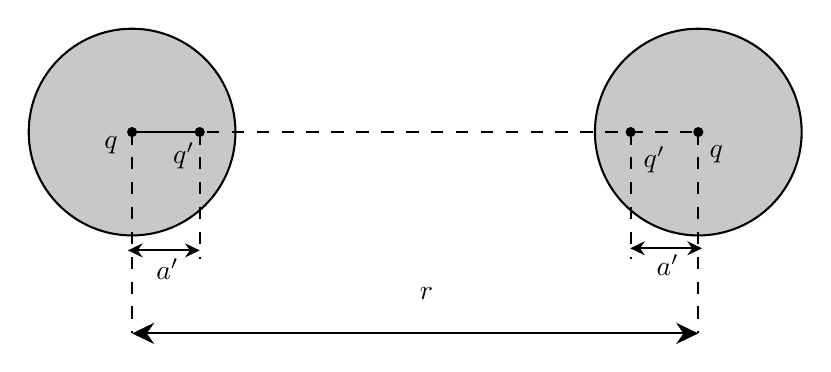
\begin{tikzpicture}[x=0.75pt,y=0.75pt,yscale=-1,xscale=1]
%uncomment if require: \path (0,300); %set diagram left start at 0, and has height of 300

%Shape: Circle [id:dp8017741508820471] 
\draw  [fill={rgb, 255:red, 200; green, 200; blue, 200 }  ,fill opacity=1 ] (119,118.8) .. controls (119,91.3) and (141.3,69) .. (168.8,69) .. controls (196.3,69) and (218.6,91.3) .. (218.6,118.8) .. controls (218.6,146.3) and (196.3,168.6) .. (168.8,168.6) .. controls (141.3,168.6) and (119,146.3) .. (119,118.8) -- cycle ;
%Shape: Circle [id:dp7664923549800668] 
\draw  [fill={rgb, 255:red, 200; green, 200; blue, 200 }  ,fill opacity=1 ] (391.8,118.8) .. controls (391.8,91.3) and (414.1,69) .. (441.6,69) .. controls (469.1,69) and (491.4,91.3) .. (491.4,118.8) .. controls (491.4,146.3) and (469.1,168.6) .. (441.6,168.6) .. controls (414.1,168.6) and (391.8,146.3) .. (391.8,118.8) -- cycle ;
%Straight Lines [id:da33322088243625014] 
\draw  [dash pattern={on 4.5pt off 4.5pt}]  (168.8,118.8) -- (441.6,118.8) ;
%Straight Lines [id:da19243486235427976] 
\draw  [dash pattern={on 4.5pt off 4.5pt}]  (168.8,118.8) -- (168.8,215.8) ;
%Straight Lines [id:da838299476811518] 
\draw  [dash pattern={on 4.5pt off 4.5pt}]  (441.6,118.8) -- (441.6,215.8) ;
%Straight Lines [id:da15857420082011497] 
\draw    (171.8,215.8) -- (438.6,215.8) ;
\draw [shift={(441.6,215.8)}, rotate = 180] [fill={rgb, 255:red, 0; green, 0; blue, 0 }  ][line width=0.08]  [draw opacity=0] (10.72,-5.15) -- (0,0) -- (10.72,5.15) -- (7.12,0) -- cycle    ;
\draw [shift={(168.8,215.8)}, rotate = 0] [fill={rgb, 255:red, 0; green, 0; blue, 0 }  ][line width=0.08]  [draw opacity=0] (10.72,-5.15) -- (0,0) -- (10.72,5.15) -- (7.12,0) -- cycle    ;
%Straight Lines [id:da47706538631258133] 
\draw    (168.8,118.8) -- (201.4,118.8) ;
%Straight Lines [id:da14110892575851053] 
\draw  [dash pattern={on 4.5pt off 4.5pt}]  (409,118.8) -- (409,179.8) ;
%Shape: Circle [id:dp8698776366930043] 
\draw  [color={rgb, 255:red, 0; green, 0; blue, 0 }  ,draw opacity=1 ][fill={rgb, 255:red, 0; green, 0; blue, 0 }  ,fill opacity=1 ] (199.5,118.8) .. controls (199.5,117.75) and (200.35,116.9) .. (201.4,116.9) .. controls (202.45,116.9) and (203.3,117.75) .. (203.3,118.8) .. controls (203.3,119.85) and (202.45,120.7) .. (201.4,120.7) .. controls (200.35,120.7) and (199.5,119.85) .. (199.5,118.8) -- cycle ;
%Straight Lines [id:da5575708691384333] 
\draw  [dash pattern={on 4.5pt off 4.5pt}]  (201.4,118.8) -- (201.4,179.8) ;
%Straight Lines [id:da5329732710897337] 
\draw    (169.8,175.8) -- (198.4,175.8) ;
\draw [shift={(201.4,175.8)}, rotate = 180] [fill={rgb, 255:red, 0; green, 0; blue, 0 }  ][line width=0.08]  [draw opacity=0] (7.14,-3.43) -- (0,0) -- (7.14,3.43) -- (4.74,0) -- cycle    ;
\draw [shift={(166.8,175.8)}, rotate = 0] [fill={rgb, 255:red, 0; green, 0; blue, 0 }  ][line width=0.08]  [draw opacity=0] (7.14,-3.43) -- (0,0) -- (7.14,3.43) -- (4.74,0) -- cycle    ;
%Straight Lines [id:da39987258639683065] 
\draw    (411.8,174.8) -- (440.4,174.8) ;
\draw [shift={(443.4,174.8)}, rotate = 180] [fill={rgb, 255:red, 0; green, 0; blue, 0 }  ][line width=0.08]  [draw opacity=0] (7.14,-3.43) -- (0,0) -- (7.14,3.43) -- (4.74,0) -- cycle    ;
\draw [shift={(408.8,174.8)}, rotate = 0] [fill={rgb, 255:red, 0; green, 0; blue, 0 }  ][line width=0.08]  [draw opacity=0] (7.14,-3.43) -- (0,0) -- (7.14,3.43) -- (4.74,0) -- cycle    ;
%Shape: Circle [id:dp6776066140031742] 
\draw  [color={rgb, 255:red, 0; green, 0; blue, 0 }  ,draw opacity=1 ][fill={rgb, 255:red, 0; green, 0; blue, 0 }  ,fill opacity=1 ] (166.9,118.8) .. controls (166.9,117.75) and (167.75,116.9) .. (168.8,116.9) .. controls (169.85,116.9) and (170.7,117.75) .. (170.7,118.8) .. controls (170.7,119.85) and (169.85,120.7) .. (168.8,120.7) .. controls (167.75,120.7) and (166.9,119.85) .. (166.9,118.8) -- cycle ;
%Shape: Circle [id:dp15849887008272545] 
\draw  [color={rgb, 255:red, 0; green, 0; blue, 0 }  ,draw opacity=1 ][fill={rgb, 255:red, 0; green, 0; blue, 0 }  ,fill opacity=1 ] (407.1,118.8) .. controls (407.1,117.75) and (407.95,116.9) .. (409,116.9) .. controls (410.05,116.9) and (410.9,117.75) .. (410.9,118.8) .. controls (410.9,119.85) and (410.05,120.7) .. (409,120.7) .. controls (407.95,120.7) and (407.1,119.85) .. (407.1,118.8) -- cycle ;
%Shape: Circle [id:dp0720499267724688] 
\draw  [color={rgb, 255:red, 0; green, 0; blue, 0 }  ,draw opacity=1 ][fill={rgb, 255:red, 0; green, 0; blue, 0 }  ,fill opacity=1 ] (439.7,118.8) .. controls (439.7,117.75) and (440.55,116.9) .. (441.6,116.9) .. controls (442.65,116.9) and (443.5,117.75) .. (443.5,118.8) .. controls (443.5,119.85) and (442.65,120.7) .. (441.6,120.7) .. controls (440.55,120.7) and (439.7,119.85) .. (439.7,118.8) -- cycle ;


% Text Node
\draw (154,119.4) node [anchor=north west][inner sep=0.75pt]    {$q$};
% Text Node
\draw (187.1,122.2) node [anchor=north west][inner sep=0.75pt]    {$q'$};
% Text Node
\draw (445.6,124) node [anchor=north west][inner sep=0.75pt]    {$q$};
% Text Node
\draw (413.8,124.2) node [anchor=north west][inner sep=0.75pt]    {$q'$};
% Text Node
\draw (179,178.4) node [anchor=north west][inner sep=0.75pt]    {$a'$};
% Text Node
\draw (420,176.4) node [anchor=north west][inner sep=0.75pt]    {$a'$};
% Text Node
\draw (306,192.4) node [anchor=north west][inner sep=0.75pt]    {$r$};


\end{tikzpicture}
\end{center}

Ở bậc đầu tiên, điện tích $q$ ở tâm mỗi quả cầu sẽ hưởng ứng và tạo ra một điện tích ảnh $q^\prime = -\alpha q$ bên trong mặt cầu còn lại, đặt ở khoảng cách $a’ = a^2/r = r \alpha^2$ từ tâm của nó, (xem hình vẽ). Do đó, bằng cách giải hệ phương trình $q^\prime=-\alpha q$, và $q+q’=Q$, chúng ta thu được độ lớn của mỗi điện tích:\\
   \[ q = \frac{1}{1-\alpha}Q, \quad q’ = - \frac{\alpha}{1- \alpha}Q. \tag{1} \]

   \begin{center}


\tikzset{every picture/.style={line width=0.75pt}} %set default line width to 0.75pt        

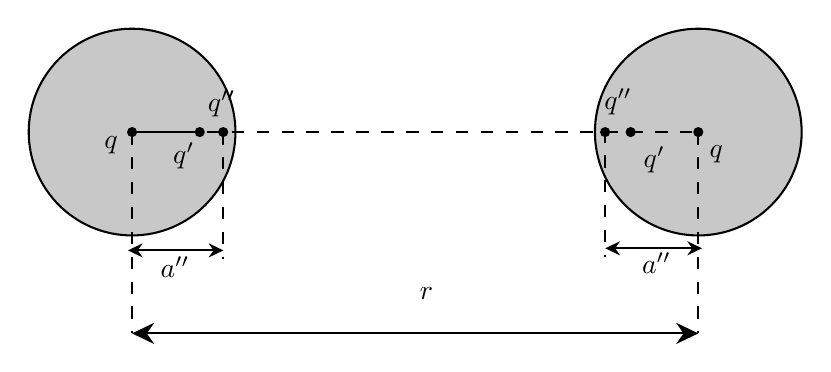
\begin{tikzpicture}[x=0.75pt,y=0.75pt,yscale=-1,xscale=1]
%uncomment if require: \path (0,300); %set diagram left start at 0, and has height of 300

%Shape: Circle [id:dp34348284742580737] 
\draw  [fill={rgb, 255:red, 200; green, 200; blue, 200 }  ,fill opacity=1 ] (119,118.8) .. controls (119,91.3) and (141.3,69) .. (168.8,69) .. controls (196.3,69) and (218.6,91.3) .. (218.6,118.8) .. controls (218.6,146.3) and (196.3,168.6) .. (168.8,168.6) .. controls (141.3,168.6) and (119,146.3) .. (119,118.8) -- cycle ;
%Shape: Circle [id:dp7046735298451712] 
\draw  [fill={rgb, 255:red, 200; green, 200; blue, 200}  ,fill opacity=1 ] (391.8,118.8) .. controls (391.8,91.3) and (414.1,69) .. (441.6,69) .. controls (469.1,69) and (491.4,91.3) .. (491.4,118.8) .. controls (491.4,146.3) and (469.1,168.6) .. (441.6,168.6) .. controls (414.1,168.6) and (391.8,146.3) .. (391.8,118.8) -- cycle ;
%Straight Lines [id:da43807453833658716] 
\draw  [dash pattern={on 4.5pt off 4.5pt}]  (168.8,118.8) -- (441.6,118.8) ;
%Straight Lines [id:da2497826794596627] 
\draw  [dash pattern={on 4.5pt off 4.5pt}]  (168.8,118.8) -- (168.8,215.8) ;
%Straight Lines [id:da5697190603484226] 
\draw  [dash pattern={on 4.5pt off 4.5pt}]  (441.6,118.8) -- (441.6,215.8) ;
%Straight Lines [id:da9417430605947157] 
\draw    (171.8,215.8) -- (438.6,215.8) ;
\draw [shift={(441.6,215.8)}, rotate = 180] [fill={rgb, 255:red, 0; green, 0; blue, 0 }  ][line width=0.08]  [draw opacity=0] (10.72,-5.15) -- (0,0) -- (10.72,5.15) -- (7.12,0) -- cycle    ;
\draw [shift={(168.8,215.8)}, rotate = 0] [fill={rgb, 255:red, 0; green, 0; blue, 0 }  ][line width=0.08]  [draw opacity=0] (10.72,-5.15) -- (0,0) -- (10.72,5.15) -- (7.12,0) -- cycle    ;
%Straight Lines [id:da462000380522237] 
\draw    (168.8,118.8) -- (201.4,118.8) ;
%Straight Lines [id:da18145437963575572] 
\draw  [dash pattern={on 4.5pt off 4.5pt}]  (396.7,117.9) -- (396.7,178.9) ;
%Shape: Circle [id:dp15554898972233078] 
\draw  [color={rgb, 255:red, 0; green, 0; blue, 0 }  ,draw opacity=1 ][fill={rgb, 255:red, 0; green, 0; blue, 0 }  ,fill opacity=1 ] (199.5,118.8) .. controls (199.5,117.75) and (200.35,116.9) .. (201.4,116.9) .. controls (202.45,116.9) and (203.3,117.75) .. (203.3,118.8) .. controls (203.3,119.85) and (202.45,120.7) .. (201.4,120.7) .. controls (200.35,120.7) and (199.5,119.85) .. (199.5,118.8) -- cycle ;
%Straight Lines [id:da23915758197960524] 
\draw  [dash pattern={on 4.5pt off 4.5pt}]  (212.8,118.8) -- (212.8,179.8) ;
%Straight Lines [id:da7991231486525425] 
\draw    (169.8,175.8) -- (209.8,175.8) ;
\draw [shift={(212.8,175.8)}, rotate = 180] [fill={rgb, 255:red, 0; green, 0; blue, 0 }  ][line width=0.08]  [draw opacity=0] (7.14,-3.43) -- (0,0) -- (7.14,3.43) -- (4.74,0) -- cycle    ;
\draw [shift={(166.8,175.8)}, rotate = 0] [fill={rgb, 255:red, 0; green, 0; blue, 0 }  ][line width=0.08]  [draw opacity=0] (7.14,-3.43) -- (0,0) -- (7.14,3.43) -- (4.74,0) -- cycle    ;
%Straight Lines [id:da9243844882843539] 
\draw    (399.8,174.8) -- (440.4,174.8) ;
\draw [shift={(443.4,174.8)}, rotate = 180] [fill={rgb, 255:red, 0; green, 0; blue, 0 }  ][line width=0.08]  [draw opacity=0] (7.14,-3.43) -- (0,0) -- (7.14,3.43) -- (4.74,0) -- cycle    ;
\draw [shift={(396.8,174.8)}, rotate = 0] [fill={rgb, 255:red, 0; green, 0; blue, 0 }  ][line width=0.08]  [draw opacity=0] (7.14,-3.43) -- (0,0) -- (7.14,3.43) -- (4.74,0) -- cycle    ;
%Shape: Circle [id:dp9988955107995567] 
\draw  [color={rgb, 255:red, 0; green, 0; blue, 0 }  ,draw opacity=1 ][fill={rgb, 255:red, 0; green, 0; blue, 0 }  ,fill opacity=1 ] (166.9,118.8) .. controls (166.9,117.75) and (167.75,116.9) .. (168.8,116.9) .. controls (169.85,116.9) and (170.7,117.75) .. (170.7,118.8) .. controls (170.7,119.85) and (169.85,120.7) .. (168.8,120.7) .. controls (167.75,120.7) and (166.9,119.85) .. (166.9,118.8) -- cycle ;
%Shape: Circle [id:dp22303428223520694] 
\draw  [color={rgb, 255:red, 0; green, 0; blue, 0 }  ,draw opacity=1 ][fill={rgb, 255:red, 0; green, 0; blue, 0 }  ,fill opacity=1 ] (407.1,118.8) .. controls (407.1,117.75) and (407.95,116.9) .. (409,116.9) .. controls (410.05,116.9) and (410.9,117.75) .. (410.9,118.8) .. controls (410.9,119.85) and (410.05,120.7) .. (409,120.7) .. controls (407.95,120.7) and (407.1,119.85) .. (407.1,118.8) -- cycle ;
%Shape: Circle [id:dp5781597284030657] 
\draw  [color={rgb, 255:red, 0; green, 0; blue, 0 }  ,draw opacity=1 ][fill={rgb, 255:red, 0; green, 0; blue, 0 }  ,fill opacity=1 ] (439.7,118.8) .. controls (439.7,117.75) and (440.55,116.9) .. (441.6,116.9) .. controls (442.65,116.9) and (443.5,117.75) .. (443.5,118.8) .. controls (443.5,119.85) and (442.65,120.7) .. (441.6,120.7) .. controls (440.55,120.7) and (439.7,119.85) .. (439.7,118.8) -- cycle ;
%Shape: Circle [id:dp966763657705122] 
\draw  [color={rgb, 255:red, 0; green, 0; blue, 0 }  ,draw opacity=1 ][fill={rgb, 255:red, 0; green, 0; blue, 0 }  ,fill opacity=1 ] (210.8,118.8) .. controls (210.8,117.75) and (211.65,116.9) .. (212.7,116.9) .. controls (213.75,116.9) and (214.6,117.75) .. (214.6,118.8) .. controls (214.6,119.85) and (213.75,120.7) .. (212.7,120.7) .. controls (211.65,120.7) and (210.8,119.85) .. (210.8,118.8) -- cycle ;
%Shape: Circle [id:dp5621567874152638] 
\draw  [color={rgb, 255:red, 0; green, 0; blue, 0 }  ,draw opacity=1 ][fill={rgb, 255:red, 0; green, 0; blue, 0 }  ,fill opacity=1 ] (394.8,118.8) .. controls (394.8,117.75) and (395.65,116.9) .. (396.7,116.9) .. controls (397.75,116.9) and (398.6,117.75) .. (398.6,118.8) .. controls (398.6,119.85) and (397.75,120.7) .. (396.7,120.7) .. controls (395.65,120.7) and (394.8,119.85) .. (394.8,118.8) -- cycle ;


% Text Node
\draw (154,119.4) node [anchor=north west][inner sep=0.75pt]    {$q$};
% Text Node
\draw (187.1,122.2) node [anchor=north west][inner sep=0.75pt]    {$q'$};
% Text Node
\draw (445.6,124) node [anchor=north west][inner sep=0.75pt]    {$q$};
% Text Node
\draw (413.8,124.2) node [anchor=north west][inner sep=0.75pt]    {$q'$};
% Text Node
\draw (181,177.4) node [anchor=north west][inner sep=0.75pt]    {$a''$};
% Text Node
\draw (413,175.4) node [anchor=north west][inner sep=0.75pt]    {$a''$};
% Text Node
\draw (306,192.4) node [anchor=north west][inner sep=0.75pt]    {$r$};
% Text Node
\draw (203.8,97.2) node [anchor=north west][inner sep=0.75pt]    {$q''$};
% Text Node
\draw (394.8,96.2) node [anchor=north west][inner sep=0.75pt]    {$q''$};


\end{tikzpicture}
\end{center}

Ở bậc độ lớn thứ hai, điện tích bậc nhất $q^{\prime}$ bên trong mỗi quả cầu lại tạo ra điện tích ảnh $q^{\prime \prime}$ bên trong mặt cầu còn lại, đặt ở khoảng cách $a^{\prime \prime}$ từ tâm mặt cầu, (xem hình vẽ). Vì khoảng cách của $q^\prime$ đến tâm của mặt cầu còn lại là $r-a^{\prime} = r(1-\alpha^2)$, ta có:\\
 \[q^{\prime \prime} = - q’ \frac{a}{r-a’} = -q’ \frac{\alpha}{1-\alpha^2}, \quad a''=\frac{a^2}{r-a’} = r\frac{\alpha^2}{1-\alpha^2}. \tag{2}\]
 
Kết hợp phương trình trên cho $q^{\prime \prime}$ với $q^\prime= - \alpha q$ và $q+q^\prime +q^{\prime \prime}=Q$, cuối cùng ta thu được:
    \[q = Q\frac{1 - \alpha^2}{ 1 - \alpha +\alpha^3}, \quad q’ = -Q \frac{\alpha(1-\alpha^2)}{1-\alpha + \alpha^3} , \quad q^{\prime \prime}= Q \frac{\alpha^2}{1-\alpha + \alpha^3}. \tag{3} \]

Các bậc bổ chính cao hơn có thể được tính với phương pháp tương tự. Do đó, chúng ta thu được một chuỗi các điện tích ảnh $q,q^\prime,q^{\prime \prime},q^{\prime \prime \prime},...$ bên trong mỗi mặt cầu. Ở mỗi lần hưởng ứng, điện tích ảnh mới sẽ nhân thêm một hệ số $\alpha$ so với điện tích trước đó. Do đó, thông số $\alpha/r$ càng nhỏ, chúng ta càng dễ dàng để thu được một xấp xỉ chính xác.
  \item Chúng ta tính bổ chính bậc nhất của lực giữa hai quả cầu bằng cách chỉ thêm vào điện tích ảnh ở $(1)$ cho mỗi quả cầu. Với cách xấp xỉ này, lực tương tác giữa hai mặt cầu bao gồm bốn thành phần. Thành phần đầu tiên là tương tác giữa hai điện tích bậc không $q$. Thành phần thứ hai và ba là tương tác của điện tích bậc không $q$ và điện tích bậc nhất $q^\prime$ ở mặt cầu còn lại. Thành phần thứ tư là tương tác giữa hai điện tích bậc nhất $q’$, được đặt ở khoảng cách $r-2\alpha^\prime = r(1-2\alpha^2) $ so với nhau. Cộng tất cả các tương tác ta thu được:
  \[ F = k_e \frac{Q^2}{r^2} \frac{1}{(1-\alpha)^2} \left[ 1 - \frac{2\alpha}{(1-\alpha^2)^2} + \left(\frac{\alpha}{1 -2\alpha^2}\right)^2 \right] . \tag{4} \]

Sử dụng khai triển Taylor đối với $x<1$,
   \[\frac{1}{(1-x)^2} = 1 + 2x + 3x^2 + 4x^3 + O(x^4) , \tag{5} \]

chúng ta khai triển cho đến bậc bốn,
   \[\frac{1}{(1-\alpha^2)^2} = 1 + 2\alpha^2 + 3\alpha^4 + O(\alpha^6), \tag{6} \]

và
  \[\frac{1}{(1-2\alpha^2)^2} = 1 + 4\alpha^2 + 12\alpha^4+ O(\alpha^6), \tag{7} \]

do đó:
  \[\begin{aligned} F &= k_e \frac{Q^2}{r^2} ( 1 + 2\alpha +3\alpha^2 + 4\alpha^3 + …)(1 - 2\alpha + \alpha^2 -4\alpha^3 +...)\\
   &= k_e \frac{Q^2}{r^2}[ 1 - 4\alpha^3 + O(\alpha^4)], \end{aligned} \tag{8} \]

tất cả các thành phần chứa $\alpha$ và $\alpha^2$ đều triệt tiêu. Do đó, bổ chính bậc đầu tiên cho định luật Coulomb sẽ chứa bậc ba của $a/r$,
   \[F = k_e \frac{Q^2}{r^2}\left(1 -4 \frac{a^3}{r^3}\right) . \tag{9} \]

Kết quả này có thể được diễn giải bằng cách khai triển đa cực của phân bố điện tích trên mỗi quả cầu. Đa cực đầu tiên của phân bố điện tích trên quả cầu là một đơn cực tương ứng với điện tích $Q$, và một lưỡng cực $\ot{p} = -q^\prime a^\prime \hat{r} = - (\alpha Q)(\alpha^2 r)\hat{r} = -\alpha^3 Q r \hat{r}, $ với $\hat{r}$ hướng theo phương nối tâm của hai quả cầu. Đóng góp của đơn cực cho lực tương tác là $F_{mm} = k_e Q^2/r^2 .$ Bây giờ chúng ta cần tính lực tương tác của mỗi đơn cực lên lưỡng cực ở mặt cầu còn lại. Đơn cực ở quả cầu bên trái gây ra một điện trường $\ot{E}^{(0)} = k_e Q/r^2$ ở tâm của quả cầu bên phải. Chúng ta có thể tính moment lưỡng cực ở quả cầu bên phải với giới hạn $h\rightarrow 0$ của hai điện tích, $-q^\prime$ đặt tại $r-h$ từ tâm của quả cầu thứ nhất và $q^\prime$ đặt tại $r$, với $q^\prime h = |p|.$ Lực giữa đơn cực bên trái và lưỡng cực bên phải là:
   \[\begin{aligned}
F_{\mathrm{md}} &=\lim _{h \rightarrow 0} k_{\mathrm{e}} Q q^{\prime}\left[-\frac{1}{(r-h)^{2}}+\frac{1}{r^{2}}\right] \simeq \lim _{h \rightarrow 0} k_{\mathrm{e}} Q q^{\prime}\left(-\frac{1}{r^{2}}-\frac{2 h}{r^{3}}+\frac{1}{r^{2}}\right) \\
&=-\lim _{h \rightarrow 0} k_{\mathrm{e}} Q q^{\prime} \frac{2 h}{r^{3}}=-2 k_{\mathrm{e}} \frac{Q p}{r^{3}}=-2 k_{\mathrm{e}} \alpha^{3} \frac{Q^{2}}{r^{3}}.
\end{aligned} \tag{10}\]
ở đây chúng ta đã sử dụng khai triển Taylor bậc nhất cho $(r-h)^{-2}$. Bổ sung lực giữa đơn cực bên phải và lưỡng cực bên trái, tổng lực tương tác là:
  \[ F= F_{mm} + 2F{md} = k_e \frac{Q^2}{r^2}\left(1 - 4 \frac{a^3}{r^3}\right), \tag{11} \]

giống kết quả của phương trình $(9)$. Kết quả tương tự cũng thu được bằng cách áp dụng công thức lực giữa điện tích điểm và một lưỡng cực điện $\ot{F} = (\ot{p} \cdot \nabla) \ot{E}$. \\
Từ $(9)$, chúng ta thấy rằng ở tỉ lệ $a/r \approx 0.13$ là đủ để sai số của phép đo ở mức dưới $1\%$.
\end{enumerate}
\end{loigiai}

\begin{vd}[Lực giữa một vỏ cầu dẫn và một mặt phẳng dẫn]\\
Định lý độc đáo về lý thuyết điện trường khẳng định rằng các điện tích ảnh có thể được đặt bên ngoài không gian kín, nơi mà điện trường được xác định bằng cách ``bắt chước'' các điều kiện biên thực. Ví dụ như, trong hình $A$ dưới đây, để tìm điện trường khi một điện tích $q$ được đặt ở trước một mặt phẳng dẫn có điện thế bằng không, một điện tích ảo (hay ảnh) có điện tích $-q$ được đặt tại điểm đối xứng với $q$ qua gương. Sự kết hợp của hai điện tích như vậy tạo ra điện thế ở khắp mọi nơi trên mặt phẳng không. Lực tác dụng lên $q$ bởi mặt phẳng giống như lực bởi điện tích ảnh.\\
\begin{center}


% Gradient Info
  
\tikzset {_pcq0kpp3g/.code = {\pgfsetadditionalshadetransform{ \pgftransformshift{\pgfpoint{0 bp } { 0 bp }  }  \pgftransformscale{1 }  }}}
\pgfdeclareradialshading{_jrmgez7us}{\pgfpoint{0bp}{0bp}}{rgb(0bp)=(1,1,1);
rgb(0bp)=(1,1,1);
rgb(25bp)=(0,0,0);
rgb(400bp)=(0,0,0)}
\tikzset{every picture/.style={line width=0.75pt}} %set default line width to 0.75pt        

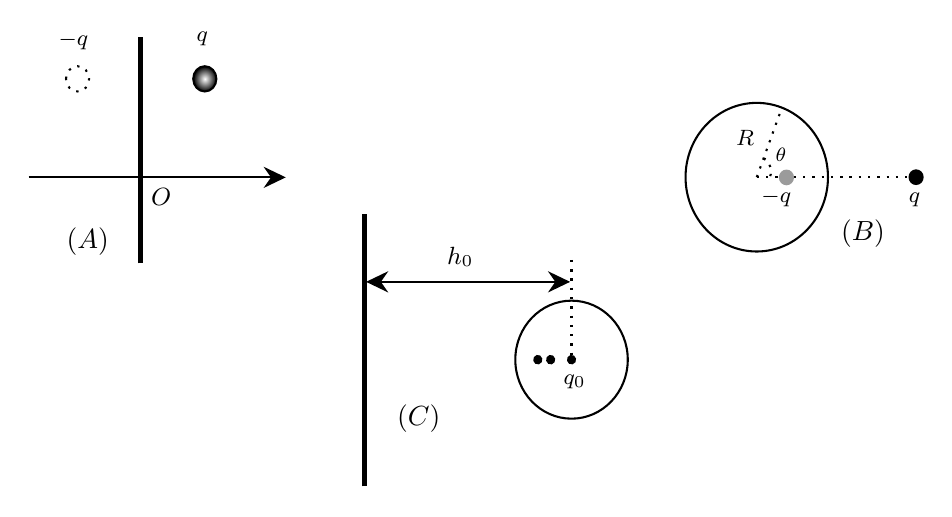
\begin{tikzpicture}[x=0.75pt,y=0.75pt,yscale=-1,xscale=1]
%uncomment if require: \path (0,300); %set diagram left start at 0, and has height of 300

%Straight Lines [id:da6601714456814607] 
\draw    (5,93.45) -- (125.85,93.45) ;
\draw [shift={(128.85,93.45)}, rotate = 180] [fill={rgb, 255:red, 0; green, 0; blue, 0 }  ][line width=0.08]  [draw opacity=0] (10.72,-5.15) -- (0,0) -- (10.72,5.15) -- (7.12,0) -- cycle    ;
%Straight Lines [id:da08606382912317101] 
\draw [line width=1.5]    (58.87,134.85) -- (58.87,25.73) ;
%Shape: Ellipse [id:dp2888561445190583] 
\path  [shading=_jrmgez7us,_pcq0kpp3g] (84.26,45.98) .. controls (84.26,42.63) and (86.76,39.91) .. (89.84,39.91) .. controls (92.91,39.91) and (95.41,42.63) .. (95.41,45.98) .. controls (95.41,49.34) and (92.91,52.06) .. (89.84,52.06) .. controls (86.76,52.06) and (84.26,49.34) .. (84.26,45.98) -- cycle ; % for fading 
 \draw   (84.26,45.98) .. controls (84.26,42.63) and (86.76,39.91) .. (89.84,39.91) .. controls (92.91,39.91) and (95.41,42.63) .. (95.41,45.98) .. controls (95.41,49.34) and (92.91,52.06) .. (89.84,52.06) .. controls (86.76,52.06) and (84.26,49.34) .. (84.26,45.98) -- cycle ; % for border 

%Shape: Ellipse [id:dp17235475214944218] 
\draw  [dash pattern={on 0.84pt off 2.51pt}] (22.96,45.98) .. controls (22.96,42.63) and (25.45,39.91) .. (28.53,39.91) .. controls (31.61,39.91) and (34.1,42.63) .. (34.1,45.98) .. controls (34.1,49.34) and (31.61,52.06) .. (28.53,52.06) .. controls (25.45,52.06) and (22.96,49.34) .. (22.96,45.98) -- cycle ;
%Shape: Ellipse [id:dp6216506123046832] 
\draw   (321.46,93.36) .. controls (321.46,73.59) and (336.82,57.56) .. (355.77,57.56) .. controls (374.72,57.56) and (390.08,73.59) .. (390.08,93.36) .. controls (390.08,113.13) and (374.72,129.17) .. (355.77,129.17) .. controls (336.82,129.17) and (321.46,113.13) .. (321.46,93.36) -- cycle ;
%Straight Lines [id:da2346616933405914] 
\draw  [dash pattern={on 0.84pt off 2.51pt}]  (355.77,93.36) -- (432.53,93.36) ;
%Shape: Ellipse [id:dp2834209109289758] 
\draw  [color={rgb, 255:red, 155; green, 155; blue, 155 }  ,draw opacity=1 ][fill={rgb, 255:red, 155; green, 155; blue, 155 }  ,fill opacity=1 ] (366.93,93.48) .. controls (366.93,91.67) and (368.34,90.2) .. (370.08,90.2) .. controls (371.81,90.2) and (373.22,91.67) .. (373.22,93.48) .. controls (373.22,95.29) and (371.81,96.76) .. (370.08,96.76) .. controls (368.34,96.76) and (366.93,95.29) .. (366.93,93.48) -- cycle ;
%Shape: Ellipse [id:dp21514597700929183] 
\draw  [color={rgb, 255:red, 0; green, 0; blue, 0 }  ,draw opacity=1 ][fill={rgb, 255:red, 0; green, 0; blue, 0 }  ,fill opacity=1 ] (429.39,93.36) .. controls (429.39,91.55) and (430.8,90.08) .. (432.53,90.08) .. controls (434.27,90.08) and (435.68,91.55) .. (435.68,93.36) .. controls (435.68,95.17) and (434.27,96.64) .. (432.53,96.64) .. controls (430.8,96.64) and (429.39,95.17) .. (429.39,93.36) -- cycle ;
%Straight Lines [id:da356631415345922] 
\draw  [dash pattern={on 0.84pt off 2.51pt}]  (355.77,93.36) -- (367.63,60.59) ;
%Curve Lines [id:da8606118783623455] 
\draw  [dash pattern={on 0.84pt off 2.51pt}]  (359.26,85.11) .. controls (359.96,82.44) and (364.14,89.72) .. (362.05,93.36) ;
%Straight Lines [id:da9691264527187986] 
\draw [line width=1.5]    (166.78,242.33) -- (166.78,111.03) ;
%Shape: Ellipse [id:dp3825983617890736] 
\draw   (239.44,181.28) .. controls (239.44,165.58) and (251.57,152.85) .. (266.53,152.85) .. controls (281.49,152.85) and (293.62,165.58) .. (293.62,181.28) .. controls (293.62,196.98) and (281.49,209.71) .. (266.53,209.71) .. controls (251.57,209.71) and (239.44,196.98) .. (239.44,181.28) -- cycle ;
%Shape: Ellipse [id:dp152854412227321] 
\draw  [fill={rgb, 255:red, 0; green, 0; blue, 0 }  ,fill opacity=1 ] (268.18,180.88) .. controls (267.96,179.92) and (267.05,179.33) .. (266.14,179.55) .. controls (265.23,179.77) and (264.67,180.73) .. (264.88,181.68) .. controls (265.09,182.64) and (266,183.23) .. (266.91,183.01) .. controls (267.82,182.79) and (268.39,181.83) .. (268.18,180.88) -- cycle ;
%Shape: Ellipse [id:dp3529840840738634] 
\draw  [fill={rgb, 255:red, 0; green, 0; blue, 0 }  ,fill opacity=1 ] (258.11,180.88) .. controls (257.9,179.92) and (256.99,179.33) .. (256.08,179.55) .. controls (255.17,179.77) and (254.6,180.73) .. (254.82,181.68) .. controls (255.03,182.64) and (255.94,183.23) .. (256.85,183.01) .. controls (257.76,182.79) and (258.33,181.83) .. (258.11,180.88) -- cycle ;
%Shape: Ellipse [id:dp6147892326674775] 
\draw  [fill={rgb, 255:red, 0; green, 0; blue, 0 }  ,fill opacity=1 ] (251.92,180.88) .. controls (251.71,179.92) and (250.8,179.33) .. (249.89,179.55) .. controls (248.98,179.77) and (248.41,180.73) .. (248.62,181.68) .. controls (248.84,182.64) and (249.75,183.23) .. (250.66,183.01) .. controls (251.57,182.79) and (252.13,181.83) .. (251.92,180.88) -- cycle ;
%Straight Lines [id:da26821762490444634] 
\draw  [dash pattern={on 0.84pt off 2.51pt}]  (266.53,133.23) -- (266.53,181.28) ;
%Straight Lines [id:da5904982457317562] 
\draw    (262.85,143.79) -- (170.55,143.79) ;
\draw [shift={(167.55,143.79)}, rotate = 360] [fill={rgb, 255:red, 0; green, 0; blue, 0 }  ][line width=0.08]  [draw opacity=0] (10.72,-5.15) -- (0,0) -- (10.72,5.15) -- (7.12,0) -- cycle    ;
\draw [shift={(265.85,143.79)}, rotate = 180] [fill={rgb, 255:red, 0; green, 0; blue, 0 }  ][line width=0.08]  [draw opacity=0] (10.72,-5.15) -- (0,0) -- (10.72,5.15) -- (7.12,0) -- cycle    ;

% Text Node
\draw (356.54,97.53) node [anchor=north west][inner sep=0.75pt]  [font=\footnotesize]  {$-q$};
% Text Node
\draw (427.58,99.5) node [anchor=north west][inner sep=0.75pt]  [font=\footnotesize]  {$q$};
% Text Node
\draw (344.34,69.5) node [anchor=north west][inner sep=0.75pt]  [font=\footnotesize]  {$R$};
% Text Node
\draw (363.28,77.66) node [anchor=north west][inner sep=0.75pt]  [font=\scriptsize]  {$\theta $};
% Text Node
\draw (394.86,112.46) node [anchor=north west][inner sep=0.75pt]    {$( B)$};
% Text Node
\draw (205.11,125.36) node [anchor=north west][inner sep=0.75pt]  [font=\small]  {$h_{0}$};
% Text Node
\draw (261.19,186.99) node [anchor=north west][inner sep=0.75pt]  [font=\footnotesize]  {$q_{0}$};
% Text Node
\draw (180.98,201.7) node [anchor=north west][inner sep=0.75pt]    {$( C)$};
% Text Node
\draw (17.91,21.83) node [anchor=north west][inner sep=0.75pt]  [font=\footnotesize]  {$-q$};
% Text Node
\draw (84.45,21.83) node [anchor=north west][inner sep=0.75pt]  [font=\footnotesize]  {$q$};
% Text Node
\draw (62.49,97.38) node [anchor=north west][inner sep=0.75pt]  [font=\small]  {$O$};
% Text Node
\draw (21.72,116) node [anchor=north west][inner sep=0.75pt]    {$( A)$};


\end{tikzpicture}
\end{center}
\begin{enumerate}[\text{Phần} A. ]
    \item 
    %Xét một lực do một quả cầu dẫn bán kính $R$ được giữ ở điện thế không lên điện tích $q$ tại khoảng cách $d(>R)$ từ tâm hình cầu.
    Xét lực tương tác giữa quả cầu bán kính $R$ có điện thế bằng $0$ lên một điện tích $q$ ở khoảng cách $d$ $(>R)$. Điện tích ảnh $q'$ có thể ở bên trong hình cầu
    %(bên ngoài không gian bên ngoài hình cầu) 
    (hoặc bên ngoài hình cầu) và trên đường nối tâm hình cầu với điện tích $q$, như hình $B$. Sự kết hợp của $q$ và $q'$ tạo ra điện thế trên khắp bề mặt hình cầu bằng không. Tìm vị trí và giá trị của $q'$.
    \item Như hình vẽ $C$, một vấn đề thường gặp của kính hiển vi lực nguyên tử là để xác định lực lên các mẫu trên mũi thăm dò, đó là một hình cầu dẫn bán kính $R$ được mang điện thế $V$ ở khoảng cách $h_0$ từ mặt phẳng dẫn lớn có điện thế bằng không. Trong các phần tiếp theo chúng ta có thể áp dụng phương pháp ``ảnh điện'' để tìm lực đó.
    \begin{enumerate}[1) ]
        \item Chúng ta bắt đầu bằng cách đặt một điện tích điểm $q_0$ bên ngoài hình cầu sao cho bề mặt quả cầu là đẳng thế với điện thế $V$, trong khi bỏ qua ảnh hưởng của tấm dẫn. Xác định $q_0$ theo $V$ và $R$.
        \item Xác định giá trị và vị trí $(h_1)$ của $q_1$ là điện tích ảnh của $q_0$, như vậy tổng hợp điện thế của chúng tại bề mặt của mặt phẳng bằng không.
        %Xác định giá trị và vị trí $(h_1)$ của điện tích ảnh của $q_0$ và gọi nó là $q_1$, như vậy sự kết hợp của chúng làm cho bề mặt của mặt phẳng có điện thế bằng không.
        \item Sự có mặt của $q_1$ bây giờ làm cho bề mặt của quả cầu không còn đẳng thế nữa. Đặt một điện tích điểm $q_2$ bên trong quả cầu sao cho sự kết hợp của $q_0$, $q_1$ và $q_2$ làm cho điện thế ở bề mặt quả cầu lại bằng $V$. Xác định $q_2$ và vị trí của nó $h_2$.
        \item Giải lại câu $2)$ để xác định điện tích ảnh $q_3$  của $q_2$, lặp lại $3)$ để xác định điện tích ảnh $q_4$ của $q_3$. Rút ra biểu thức chung giữa $h_{2n}$ và $h_{2(n+1)}$, $q_{2n}$ và $q_{2(n+1)}$, $q_{2n+1}$ và $q_{2(n+1)+1}$, $n=0,1,2,\dots$ 
        \item Rút ra tổng hợp lực của các điện tích tác dụng lên hình cầu dưới dạng tổng của một chuỗi vô hạn các số hạng. 
        \item Giả sử lực ở phần $5)$ là $1.1\times10^{-12}~\mathrm{N}$ với $V=V_0$, $R=1.0\times10^{-8}~\mathrm{m}$, và $h_0=5.0\times10^{-8}~\mathrm{m}$, tìm lực khi $V=2V_0$, $R=1.0~\mathrm{m}$, và $h_0=5.0\mathrm{m}$. 
        \item Cho $\dfrac{R}{h_0}=\dfrac{1}{51}$, xác định lực ở phần $5)$ đạt độ chính xác $\thicksim 1 \%$, các số hạng nào cần được giữ lại?
        \item Ước tính độ lớn của sai số tương đối mắc phải do việc bỏ qua các số hạng trong phần $7)$.
    \end{enumerate}
\end{enumerate}
\end{vd}
\begin{loigiai}
\begin{enumerate}[\text{Phần} A.]
    \item Đặt một điện tích điểm $q'$ tại vị trí $x$ tính từ tâm, tại một điểm trên bề mặt hình cầu cách tâm một khoảng $r$. Khoảng cách từ điểm này đến điện tích $q$ là $L$.\\Khi đó:
    \begin{align*}
        L^2&=R^2+d^2-2Rd\mathrm{\cos{\theta}}. \tag{1} \label{cg2006sa.3.1}\\
        r^2&=R^2+x^2-2Rx\mathrm{\cos{\theta}}. \tag{2} \label{cg2006sa.3.2}
    \end{align*}
    Điện thế bằng không trên bề mặt hình cầu suy ra:
    \[\dfrac{q}{L}=-\dfrac{q'}{r}. \tag{3} \label{cg2006sa.3.3}\]
    \begin{center}


\tikzset{every picture/.style={line width=0.75pt}} %set default line width to 0.75pt        

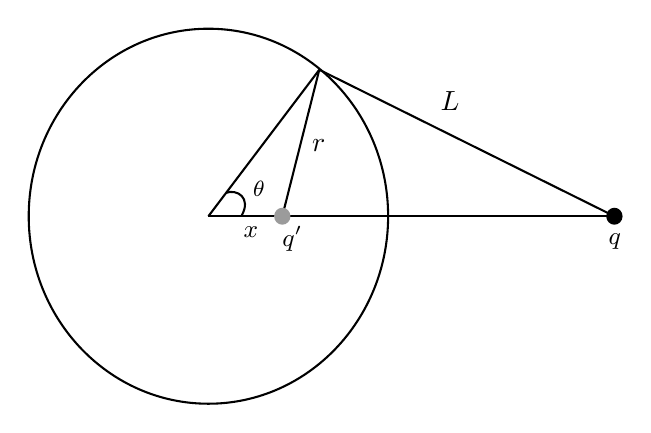
\begin{tikzpicture}[x=0.75pt,y=0.75pt,yscale=-1,xscale=1]
%uncomment if require: \path (0,300); %set diagram left start at 0, and has height of 300

%Shape: Ellipse [id:dp0350291752792955] 
\draw   (168,139.9) .. controls (168,90) and (206.76,49.56) .. (254.58,49.56) .. controls (302.39,49.56) and (341.16,90) .. (341.16,139.9) .. controls (341.16,189.8) and (302.39,230.24) .. (254.58,230.24) .. controls (206.76,230.24) and (168,189.8) .. (168,139.9) -- cycle ;
%Straight Lines [id:da6181511427117394] 
\draw    (254.58,139.9) -- (448.28,139.9) ;
%Straight Lines [id:da2802818935590121] 
\draw    (254.58,139.9) -- (308,69.33) ;
%Curve Lines [id:da3107474619793289] 
\draw    (263,128.67) .. controls (268,126.67) and (275.71,130.71) .. (270.43,139.9) ;
%Straight Lines [id:da09987033533785872] 
\draw    (308,69.33) -- (450.17,139.9) ;
%Shape: Ellipse [id:dp3331081791987791] 
\draw  [color={rgb, 255:red, 0; green, 0; blue, 0 }  ,draw opacity=1 ][fill={rgb, 255:red, 0; green, 0; blue, 0 }  ,fill opacity=1 ] (446.75,139.9) .. controls (446.75,137.93) and (448.28,136.33) .. (450.17,136.33) .. controls (452.06,136.33) and (453.6,137.93) .. (453.6,139.9) .. controls (453.6,141.88) and (452.06,143.48) .. (450.17,143.48) .. controls (448.28,143.48) and (446.75,141.88) .. (446.75,139.9) -- cycle ;
%Straight Lines [id:da14165240586809014] 
\draw    (308,69.33) -- (290.17,139.9) ;
%Shape: Ellipse [id:dp019663466176437883] 
\draw  [color={rgb, 255:red, 155; green, 155; blue, 155 }  ,draw opacity=1 ][fill={rgb, 255:red, 155; green, 155; blue, 155 }  ,fill opacity=1 ] (286.75,139.9) .. controls (286.75,137.93) and (288.28,136.33) .. (290.17,136.33) .. controls (292.06,136.33) and (293.6,137.93) .. (293.6,139.9) .. controls (293.6,141.88) and (292.06,143.48) .. (290.17,143.48) .. controls (288.28,143.48) and (286.75,141.88) .. (286.75,139.9) -- cycle ;

% Text Node
\draw (445.92,146.92) node [anchor=north west][inner sep=0.75pt]  [font=\small]  {$q$};
% Text Node
\draw (274.68,121.28) node [anchor=north west][inner sep=0.75pt]  [font=\footnotesize]  {$\theta $};
% Text Node
\draw (270,143.4) node [anchor=north west][inner sep=0.75pt]  [font=\small]  {$x$};
% Text Node
\draw (365,78.4) node [anchor=north west][inner sep=0.75pt]    {$L$};
% Text Node
\draw (303,101.4) node [anchor=north west][inner sep=0.75pt]    {$r$};
% Text Node
\draw (288.75,143.3) node [anchor=north west][inner sep=0.75pt]  [font=\small]  {$q'$};


\end{tikzpicture}
    \end{center}
    Thay phương trình (\ref{cg2006sa.3.1}) và (\ref{cg2006sa.3.2}) vào (\ref{cg2006sa.3.3}) dẫn tới:
    \[q'^{2}(R^2+d^2-2Rd\mathrm{\cos{\theta}})=q^2(R^2+x^2-2Rx\mathrm{\cos{\theta}}). \tag{4} \label{cg2006sa.3.4}\]
    Phương trình (\ref{cg2006sa.3.4}) phải đúng với mọi góc $\theta$, do đó:
    \begin{align*}
       q'^{2}(R^2+d^2) &=q^2(R^2+x^2). \tag{5} \label{cg2006sa.3.5}\\
        \text{và}~q'^2Rd\mathrm{\cos{\theta}}&=q^2Rx\mathrm{\cos{\theta}}. \tag{6} \label{cg2006sa.3.6}
    \end{align*}
    Giải phương trình (\ref{cg2006sa.3.5}) và (\ref{cg2006sa.3.6}), ta có hai nghiệm.\\
    Nghiệm thứ nhất: $x=d$ và $q'=q$. Không đúng vì $q'$ nằm bên ngoài hình cầu.\\
    Nghiệm thứ hai: $q'=\dfrac{-qR}{d}$ và $x=\dfrac{R^2}{d}<R$ (thỏa mãn).
    \item 
    \begin{enumerate}[1) ]
        \item  \[q_0=4\pi\varepsilon_0RV.\]
        \item $-q_0$ và tại một điểm ở phía bên kia của mặt phẳng cách mặt phẳng đó là $h_0$. 
        \item Sự phân bố của $q_1$ và $q_2$ là để làm cho điện thế trên bề mặt hình cầu bằng không. Câu trả lời trong phần $A$ có thể được dùng ở đây.
        \[h_2=h_0-\dfrac{R^2}{h_0+h_0}, q_2=\dfrac{R}{2h_0}q_0.\]
        \item 
        \begin{align*}
            h_{2(n+1)}&=h_0-\dfrac{R^2}{h_0+h_{2n}},\\
            q_{2(n+1)}&=\dfrac{R}{h_0+h_{2n}}q_{2n},\\
            q_{2n+1}&=-q_{2n}.
        \end{align*}
        \item Tổng tất cả các điện tích trên cả hai mặt của mặt phẳng là:
        \[F=\dfrac{-1}{4\pi\varepsilon_0}\sum_{m=0}^{\infty}\sum_{n=0}^{\infty}\dfrac{q_{2m}q_{2n}}{(h_{2m}+h_{2n})^2}.\]
        
        \item Sử dụng kết quả của ý $(1)$ và $(4)$, đặt $k\equiv\dfrac{h_0}{R}$,
        \[k_{2(n+1)}\equiv\dfrac{h_{2(n+1)}}{R}=k_0-\dfrac{1}{k_0+k_{2n}}.\]
        \[q_{2n}=\dfrac{1}{k_0+k_{2n-2}}q_{2(n-1)}=\dfrac{1}{k_0+k_{2(n-1)}}\dfrac{1}{k_0+k_{2(n-2)}}\dfrac{1}{k_0+k_{2(n-3)}}\dots q_0.\]
        Sử dụng kết quả của ý $(5)$:
        \begin{align*}
              F&=-4\pi\varepsilon_0V^2\sum_{m=0}^{\infty}\sum_{n=0}^{\infty}\dfrac{1}{(k_0+k_{2(n+1)})}\dfrac{1}{(k_0+k_{2(m+1)})}\dfrac{1}{(k_{2m}+k_{2n})^2}\\
              &\equiv-4\pi\varepsilon_0V^2g(k_0). 
        \end{align*}
      Lực này tỉ lệ với $V^2$, và chỉ phụ thuộc vào tỉ số $k_0=\dfrac{R}{h_0}$. Do đó kết quả là $4.4\times10^{-12}~\mathrm{N}$.
        \item Vì tất cả các điện tích ảnh trên bề mặt phải ở bên trong hình cầu, khoảng cách giữa hai điện tích bất kỳ bên ngoài và bên trong phải lớn hơn $2(h_0-R)$.\\
        Khi đó $h_0+h_{2n-2}>2(h_0-R)$.\\
        Do đó:
        \[\left|q_{2n}\right|=\dfrac{R}{h_0+h_{2n-2}}\left|q_{2n-2}\right|<\dfrac{R}{2(h_0-R)}\left|q_{2n-2}\right|=\dfrac{1}{100}\left|q_{2n-2}\right|,\]
        Với chỉ số hạng $n=1$ được giữ lại.
        Lực toàn phần là tổng của $q_0q_1$, $q_0q_3$, và $q_2q_1$, hay $(01)$, $(03)$, và $(12)$ rút gọn ta được:
        \[F=-\dfrac{\pi\varepsilon_0V^2}{51^2}\left(1+\dfrac{1}{51}\right).\]
        
        \item Các số hạng trong sự khai triển là bậc của $\left(\dfrac{R}{2(h_0-R)}\right)^2=(10^{-2})^2$ là $(05)$, $(23)$, $(41)$,
        \begin{align*}
            \left|F_{\mathrm{error}}\right|&=4\pi\varepsilon_0V^2\left[\dfrac{10^{-4}}{4}k_2^2+\dfrac{10^{-4}}{4\left(\dfrac{1}{k_0}+\dfrac{1}{k_4}\right)^2}+\dfrac{10^{-4}}{4\left(\dfrac{1}{k_1}+\dfrac{1}{k_5}\right)^2}\right]\\
            &<3\pi\varepsilon_0V^210^{-4}\dfrac{1}{(50)^2}.
        \end{align*}
        Những gì còn lại trong ý $(7)$ là việc tính lực là:
        \begin{align*}
             \left|F_{\mathrm{error}}\right|&<4\pi\varepsilon_0V^2\left[\dfrac{10^{-4}}{4h_2^2}+\dfrac{10^{-4}}{4(h_0+h_4)^2}+\dfrac{10^{-4}}{4(h_1+h_5)^2}\right.\\
             &\left. +\sum_{m=2}^{\infty}\sum_{n=2}^{\infty}\dfrac{1}{(h_{2m}+h_{2n})^2}\left(\dfrac{R}{2(h_0-R)}\right)^{m+n}\right]\\
             &<4\pi\varepsilon_0V^210^{-4}\left[\dfrac{3}{4(h_0-R)^2}+\sum_{m=2}^{\infty}\sum_{n=2}^{\infty}\dfrac{1}{(2h_0-2R)^2}\left(\dfrac{R}{2(h_0+R)}\right)^{m+n}\right]\\
             &<4\pi\varepsilon_0V^210^{-4}\dfrac{1}{4(h_0-R)^2}\left(3+\left(\sum_{n=0}^{\infty}\left(\dfrac{1}{100}\right)^{n}\right)^2\right)\\
             &<\dots\cong 3\pi\varepsilon_0V^210^{-4}\dfrac{1}{(h_0-R)^2}.
        \end{align*}
        Vì vậy sai số tương đối lớn nhất là: $3\times10^{-4}$.
    \end{enumerate}
\end{enumerate}
\end{loigiai}

\begin{vd}[Ảnh điện với mặt cầu úp]
Một điện tích điểm $q$ được đặt tại $x_0=\dfrac{3R}{2}$ trên trục $x$ ở phía trên của một bán cầu kim loại nối đất có bán kính $R$ trên một mặt phẳng kim loại rộng vuông góc với trục $x$ và trong mặt phẳng $y$ $-$ $z$. Tâm của bán cầu là $(0,0,0)$. Tìm thế năng của điện tích điểm.\\
(\textit{Lưu ý:} Bạn phải chứng minh các điều kiện biên được bảo toàn nếu bạn sử dụng phương pháp ảnh điện).
\begin{center}


% Pattern Info
 
\tikzset{
pattern size/.store in=\mcSize, 
pattern size = 5pt,
pattern thickness/.store in=\mcThickness, 
pattern thickness = 0.3pt,
pattern radius/.store in=\mcRadius, 
pattern radius = 1pt}
\makeatletter
\pgfutil@ifundefined{pgf@pattern@name@_q7ujn2b7h}{
\makeatletter
\pgfdeclarepatternformonly[\mcRadius,\mcThickness,\mcSize]{_q7ujn2b7h}
{\pgfpoint{-0.5*\mcSize}{-0.5*\mcSize}}
{\pgfpoint{0.5*\mcSize}{0.5*\mcSize}}
{\pgfpoint{\mcSize}{\mcSize}}
{
\pgfsetcolor{\tikz@pattern@color}
\pgfsetlinewidth{\mcThickness}
\pgfpathcircle\pgfpointorigin{\mcRadius}
\pgfusepath{stroke}
}}
\makeatother
\tikzset{every picture/.style={line width=0.75pt}} %set default line width to 0.75pt        

\begin{tikzpicture}[x=0.75pt,y=0.75pt,yscale=-1,xscale=1]
%uncomment if require: \path (0,300); %set diagram left start at 0, and has height of 300

%Shape: Path Data [id:dp10997633850070043] 
\draw  [pattern=_q7ujn2b7h,pattern size=6pt,pattern thickness=0.75pt,pattern radius=0.75pt, pattern color={rgb, 255:red, 0; green, 0; blue, 0}][line width=1.5]  (319.92,77) .. controls (354.73,77) and (382.96,105.2) .. (383.02,140) -- (470.02,140) -- (470.02,203.36) -- (170.02,203.36) -- (170.02,140) -- (256.82,140) .. controls (256.87,105.2) and (285.1,77) .. (319.92,77) -- cycle ;
%Straight Lines [id:da27042199353281826] 
\draw [color={rgb, 255:red, 236; green, 236; blue, 236 }  ,draw opacity=0.75 ][fill={rgb, 255:red, 236; green, 236; blue, 236 }  ,fill opacity=0.75 ][line width=1.5]    (170.02,140) -- (170.02,203.36) ;
%Straight Lines [id:da09108908341082844] 
\draw [color={rgb, 255:red, 236; green, 236; blue, 236 }  ,draw opacity=0.75 ][fill={rgb, 255:red, 255; green, 255; blue, 255 }  ,fill opacity=1 ][line width=1.5]    (470.02,140) -- (470.02,203.36) ;
%Straight Lines [id:da37612625831415314] 
\draw [color={rgb, 255:red, 236; green, 236; blue, 236 }  ,draw opacity=0.75 ][fill={rgb, 255:red, 255; green, 255; blue, 255 }  ,fill opacity=0.75 ][line width=1.5]    (170.02,203.36) -- (470.02,203.36) ;
%Straight Lines [id:da580663056291195] 
\draw    (320,140) -- (320,40.2) ;
\draw [shift={(320,37.2)}, rotate = 450] [fill={rgb, 255:red, 0; green, 0; blue, 0 }  ][line width=0.08]  [draw opacity=0] (10.72,-5.15) -- (0,0) -- (10.72,5.15) -- (7.12,0) -- cycle    ;

% Text Node
\draw (322,135.4) node [anchor=north west][inner sep=0.75pt]    {$O$};
% Text Node
\draw (328,27.4) node [anchor=north west][inner sep=0.75pt]    {$x$};


\end{tikzpicture}

\end{center}
\end{vd}
\begin{loigiai}
Điện tích ảnh nằm tại vị trí $x$ trên trục $x$.
\[\Phi(R)=\dfrac{1}{4\pi\varepsilon_0}\left(\dfrac{q}{\sqrt{R^2+x^2+2Rx\mathrm{\cos{\theta}}}}-\dfrac{q_1}{\sqrt{R^2+b^2+2Rb\mathrm{\cos{\theta}}}}\right)=0,\]
Hay $q^2(R^2+b^2+2Rb\mathrm{\cos{\theta}})=q_1^2(R^2+x^2+2Rx\mathrm{\cos{\theta}}).$\\
Công thức này đúng đối với góc $\theta$ bất kỳ, do đó,
\[q^2(R^2+b^2)=q_1^2(R^2+x^2). \tag{1} \label{cg.sang.2.3.1}\]
hay \[q^2b=q_1^2x. \tag{2} \label{cg.sang.2.3.2}\]
Rút gọn $b$ ta được:
\[x^2q_1^4-q^2(R^2+x^2)q_1^2+q^4R^2=0. \tag{3} \label{cg.sang.2.3.3}\]
Ta thấy hệ phương trình này có hai nghiệm, nghiệm thứ nhất là $q_1=-q$ và $x=b$, nghĩa là, điện tích điểm ảnh bên ngoài bán cầu. Vì điện tích ảnh không được đặt bên trong hình cầu, do đó không có nghiệm trong không gian đó, vì vậy không thể được sử dụng, ta bỏ đi. Nghiệm thứ hai là $q_1=-q\dfrac{R}{x}$; $b=\dfrac{R^2}{x}$, đây là giá trị và vị trí của điện tích ảnh. \\
%(Nếu không có nghiệm thứ nhất mà chỉ có nghiệm thứ hai thì cũng cho điểm tối đa.)\\
Để cho thế năng tại mặt phẳng bằng không, chúng ta cần thêm hai điện tích ảnh, cụ thể là $q_3=-q_1$ tại $-\dfrac{R^2}{x}$ và $q_3=-q$ tại $-\dfrac{3R}{2}$. Chúng ta cũng có thể thấy rằng $q_2$ và $q_3$ kết hợp sẽ làm cho điện thế trên bề mặt bán cầu bằng không.\\
Lực tác dụng lên điện tích là:
\[F_1=\dfrac{qq_1}{4\pi\varepsilon_0}\dfrac{1}{(x-b)^2}=-\dfrac{q^2}{4\pi\varepsilon_0}\dfrac{R}{x\left(x-\dfrac{R^2}{x}\right)^2}=-\dfrac{q^2}{4\pi\varepsilon_0}\dfrac{Rx}{(x^2-R^2)^2}.\]
Bây giờ để tìm thế năng, đó là năng lượng cần thiết để đưa điện tích từ vị trí vô cùng đến vị trí hiện tại.\\
Sử dụng phương pháp tính công của lực điện:
\begin{align*}
    W_1&=\int_{\dfrac{3R}{2}}^{\infty}F_1\mathrm{d}x=-\dfrac{q^2}{4\pi\varepsilon_0}\int_{\dfrac{3R}{2}}^{\infty}\dfrac{Rx}{(x^2-R^2)^2}\mathrm{d}x=-\dfrac{q^2}{8\pi\varepsilon_0}\left(\dfrac{R}{d^2-R^2}\right)\\
    &=-\dfrac{q^2}{8\pi\varepsilon_0R}\left(\dfrac{4}{9-4}\right)=-\dfrac{q^2}{10\pi\varepsilon_0R}.
\end{align*}
Bạn đọc cần chú ý rằng giá trị của thế năng này khác với kết quả tính trực tiếp thế năng tại vị trí $q_1$ do $q$ gây ra.
\[U=\dfrac{q_1}{4\pi\varepsilon_0}\dfrac{1}{(d-b)}=\dfrac{-q}{4\pi\varepsilon_0}\dfrac{R}{(d^2-R^2)}=\dfrac{-q}{5\pi\varepsilon_0R}.\]
Do đó, thế năng tĩnh điện của hệ là:
\[W=\dfrac{-q^2}{5\pi\varepsilon_0R}.\]
Đáp số của cách tính đúng bằng một nửa đáp số của cách tính sai. Nguyên nhân chính của sự khác biệt giữa hai kết quả là bởi vì giá trị của vị trí thực sự của điện tích ảnh với vị trí của điện tích thực. Do đó phương pháp để tính thế năng của điện tích là sử dụng tích phân để tính công của lực.
\begin{align*}
    W_2&=\int_{\frac{3R}{2}}^{\infty}F_2\mathrm{d}x=\dfrac{q^2}{4\pi\varepsilon_0}\int_{\frac{3R}{2}}^{\infty}\dfrac{Rx}{(x^2+R^2)^2}\mathrm{d}x=\dfrac{q^2}{8\pi\varepsilon_0R}\left(\dfrac{4}{9+4}\right)=\dfrac{q^2}{26\pi\varepsilon_0R}.\\
    W_3&=\int_{\frac{3R}{2}}^{\infty}F_3\mathrm{d}x=\dfrac{q^2}{16\pi\varepsilon_0}\int_{\frac{3R}{2}}^{\infty}\dfrac{1}{x^2}\mathrm{d}x=-\dfrac{q^2}{24\pi\varepsilon_0R}.
\end{align*}
Năng lượng tổng cộng là:
\[W=W_1+W_2+W_3=\dfrac{q^2}{2\pi\varepsilon_0R}\left(-\dfrac{1}{5}+\dfrac{1}{13}-\dfrac{1}{12}\right)=-\dfrac{161}{1560}\dfrac{q^2}{\pi\varepsilon_0R}.\]
\end{loigiai}

\begin{vd}[Lại gần rồi lại rời xa]
Một vỏ cầu dẫn điện tốt bán kính $R$ trung hòa về điện. Tâm của nó nằm ở gốc $O$ của hệ tọa độ $xOy$. Các câu trả lời được viết theo các đại lượng $L$, $R$, $Q$ và các hằng số cơ bản, với $L<R$.
\begin{enumerate}[1)]
    \item Tìm công sinh ra bởi trường tĩnh điện để di chuyển một điện tích điểm $q_1=Q$ từ tâm cầu đến $(L,0)$.
    \item Một điện tích điểm khác $q_2=\dfrac{L}{R}Q$ được đặt ở $\left(\dfrac{R^2}{L},0\right)$, tìm công sinh ra bởi trường tĩnh điện để di chuyển điện tích điểm $q_1$ từ tâm cầu đến $(L,0)$.
    \item Nếu điện tích điểm $q_1$ được đặt ở $(L,0)$, tìm công sinh ra bởi trường tĩnh điện để di chuyển điện tích điểm $q_2$ từ $(\infty,0)$ đến $\left(\dfrac{R^2}{L},0\right)$.
    \item Nếu điện tích điểm $q_1$ được đặt ở $(L,0)$, tìm công sinh ra bởi trường tĩnh điện để di chuyển điện tích điểm $q_2$ từ $(0,\infty)$ đến $\left(0,\dfrac{R^2}{L}\right)$.
\end{enumerate}
\end{vd}
\begin{loigiai}
\begin{enumerate}[1)]
    \item Sử dụng phương pháp ảnh điện ta có, điện tích ảnh và vị trí điện tích ảnh lần lượt là:
    \[q'=-\dfrac{QR}{x}~~\text{và}~~x'=\dfrac{R^2}{x}.\]
    Lực tương tác giữa điện tích $q_1$ và điện tích ảnh $q'$:
    \[f=-\dfrac{1}{4\pi\varepsilon_0}\dfrac{Qq'}{(x-x')^2}=\dfrac{1}{4\pi\varepsilon_0}\dfrac{Q^2Rx}{(x^2-R^2)^2}.\]
    Công của trường tĩnh điện khi di chuyển $q_1=Q$ từ tâm cầu đến $(L,0)$ là:
    \[W=\int_{0}^{L}f(x)\mathrm{d}x=\dfrac{1}{8\pi\varepsilon_0}\dfrac{L^2Q^2}{R(R^2-L^2)}.\]
    \item Vì điện tích bên ngoài không tạo ra bất kì điện trường nào bên trong quả cầu dẫn nên công sinh ra trong trường hợp này không khác gì với trường hợp ý $(1)$:
    \[W=\int_{0}^{L}f(x)\mathrm{d}x=\dfrac{1}{8\pi\varepsilon_0}\dfrac{L^2e^2}{R(R^2-L^2)}.\]
    \item Trường tĩnh điện tác dụng lên điện tích $q_2=\dfrac{L}{R}Q$ ở bên ngoài hình cầu dẫn tương đương với một điện trường được tạo ra bởi ba điện tích điểm $q_1=Q$ ở $(0,0)$, điện tích ảnh $q'=-\dfrac{R}{x}q_2$ ở $\ell'=\dfrac{R^2}{L},0$ và $q''=-q'_2$ tại $(0,0)$.
    \[f(x)=\dfrac{1}{4\pi\varepsilon_0}\left[\dfrac{q_2'q_2}{(x-x')^2}+\dfrac{q_2(q_1+q''_2)}{x^2}\right]=\dfrac{1}{4\pi\varepsilon_0}\left[-\dfrac{q_2^2Rx}{(x^2-R^2)^2}+\dfrac{q_2(xq_1+Rq_2)}{x^3}\right].\]
    Và công sinh ra bởi điện trường sau đó là:
    \begin{align*}
        \int_{\infty}^{\dfrac{R^2}{L}}f(x)\mathrm{d}x&=\dfrac{1}{8\pi\varepsilon_0}\left[\dfrac{L^2q^2_2}{(R^3-L^2R)}-\dfrac{Lq_2(Lq_2+2Rq_1)}{R^3}\right]\\
        &=\dfrac{1}{8\pi\varepsilon_0}\left[\dfrac{L^4Q^2}{(R^5-L^2R^3)}+\dfrac{L^2(2R^2-L^2)Q^2}{R^5}\right]\\
        &=\dfrac{1}{8\pi\varepsilon_0}\dfrac{L^2(L^4-2L^2R^2+2R^4)Q^2}{R^5(R^2-L^2)}.
    \end{align*}
    
    \item Đáp số của ý này bằng đáp số ở ý $(3)$.
\end{enumerate}
\end{loigiai}

\begin{vd}[Năng lượng lưỡng cực (G)]
    Một lưỡng cực điện với moment lưỡng cực $\ot{p}$ được đặt ở độ cao $h$ so với một mặt phẳng siêu dẫn vô hạn và lập với phương pháp tuyến mặt phẳng một góc $\theta$ như hình vẽ.
    \begin{enumerate}[1)]
        \item Xác định các thông số của lưỡng cực điện ảnh tạo ra bởi mặt phẳng và tính lực điện tác dụng lên lưỡng cực.
        \item Tính công cần thực hiện để dời lưỡng cực này ra xa vô cùng.
        \begin{center}
            

\tikzset{every picture/.style={line width=0.75pt}} %set default line width to 0.75pt        

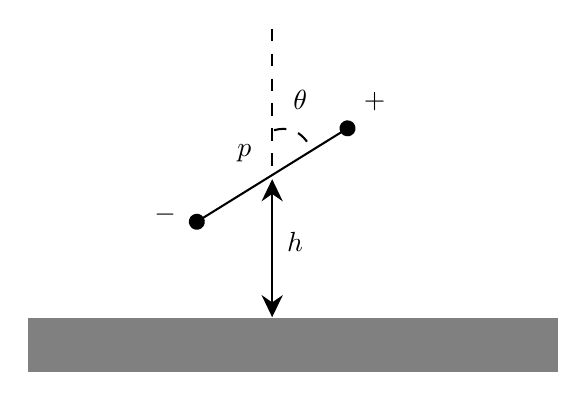
\begin{tikzpicture}[x=0.75pt,y=0.75pt,yscale=-1,xscale=1]
%uncomment if require: \path (0,575); %set diagram left start at 0, and has height of 575

%Shape: Rectangle [id:dp20102089849023264] 
\draw  [color={rgb, 255:red, 128; green, 128; blue, 128 }  ,draw opacity=1 ][fill={rgb, 255:red, 128; green, 128; blue, 128 }  ,fill opacity=1 ] (163,286) -- (417.6,286) -- (417.6,311) -- (163,311) -- cycle ;
%Straight Lines [id:da0847887713654798] 
\draw    (244,239) -- (316.6,194) ;
\draw [shift={(316.6,194)}, rotate = 328.21] [color={rgb, 255:red, 0; green, 0; blue, 0 }  ][fill={rgb, 255:red, 0; green, 0; blue, 0 }  ][line width=0.75]      (0, 0) circle [x radius= 3.35, y radius= 3.35]   ;
\draw [shift={(244,239)}, rotate = 328.21] [color={rgb, 255:red, 0; green, 0; blue, 0 }  ][fill={rgb, 255:red, 0; green, 0; blue, 0 }  ][line width=0.75]      (0, 0) circle [x radius= 3.35, y radius= 3.35]   ;
%Straight Lines [id:da5546794735087608] 
\draw  [dash pattern={on 4.5pt off 4.5pt}]  (280.3,146) -- (280.3,216.5) ;
%Straight Lines [id:da7662054730709] 
\draw    (280.3,221.5) -- (280.3,282) ;
\draw [shift={(280.3,285)}, rotate = 270] [fill={rgb, 255:red, 0; green, 0; blue, 0 }  ][line width=0.08]  [draw opacity=0] (10.72,-5.15) -- (0,0) -- (10.72,5.15) -- (7.12,0) -- cycle    ;
\draw [shift={(280.3,218.5)}, rotate = 90] [fill={rgb, 255:red, 0; green, 0; blue, 0 }  ][line width=0.08]  [draw opacity=0] (10.72,-5.15) -- (0,0) -- (10.72,5.15) -- (7.12,0) -- cycle    ;
%Shape: Arc [id:dp4483502186453965] 
\draw  [draw opacity=0][dash pattern={on 4.5pt off 4.5pt}] (281.19,194.88) .. controls (284.45,193.99) and (287.6,194.03) .. (290.48,195.13) .. controls (294.46,196.65) and (297.45,200.03) .. (299.4,204.69) -- (273.85,238.57) -- cycle ; \draw  [dash pattern={on 4.5pt off 4.5pt}] (281.19,194.88) .. controls (284.45,193.99) and (287.6,194.03) .. (290.48,195.13) .. controls (294.46,196.65) and (297.45,200.03) .. (299.4,204.69) ;


% Text Node
\draw (286,242.4) node [anchor=north west][inner sep=0.75pt]    {$h$};
% Text Node
\draw (222,229.4) node [anchor=north west][inner sep=0.75pt]    {$-$};
% Text Node
\draw (323,175.4) node [anchor=north west][inner sep=0.75pt]    {$+$};
% Text Node
\draw (262,200.4) node [anchor=north west][inner sep=0.75pt]    {$\ot{p}$};
% Text Node
\draw (289,174.4) node [anchor=north west][inner sep=0.75pt]    {$\theta $};


\end{tikzpicture}00

        \end{center}
    \end{enumerate}
\end{vd}
\begin{loigiai} 
\begin{enumerate}[1)]
   \item Bằng cách phân tích vị trí của các điện tích ảnh, ta suy ra lưỡng cực bị hút bởi mặt phẳng.
     
\begin{center}


\tikzset{every picture/.style={line width=0.75pt}} %set default line width to 0.75pt        

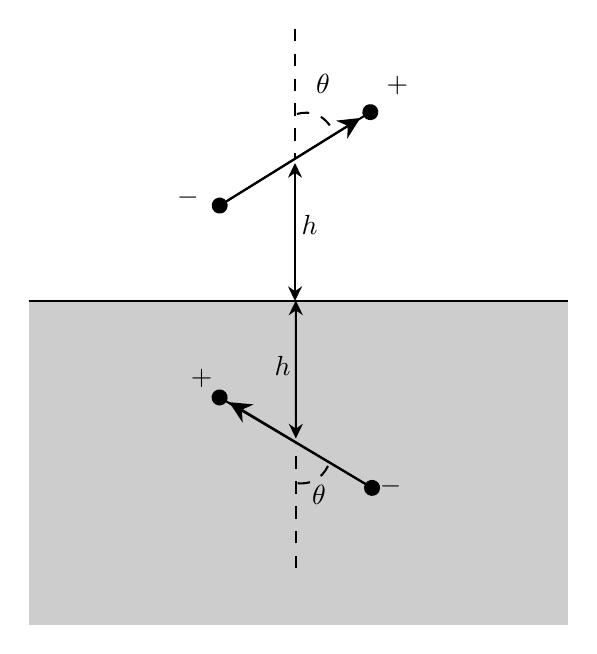
\begin{tikzpicture}[x=0.75pt,y=0.75pt,yscale=-1,xscale=1]
%uncomment if require: \path (0,575); %set diagram left start at 0, and has height of 575

%Shape: Rectangle [id:dp07003794554397302] 
\draw  [draw opacity=0][fill={rgb, 255:red, 155; green, 155; blue, 155 }  ,fill opacity=0.5 ] (152,285) -- (411.8,285) -- (411.8,441.2) -- (152,441.2) -- cycle ;
%Straight Lines [id:da14145472006648596] 
\draw    (244,239) -- (316.6,194) ;
\draw [shift={(316.6,194)}, rotate = 328.21] [color={rgb, 255:red, 0; green, 0; blue, 0 }  ][fill={rgb, 255:red, 0; green, 0; blue, 0 }  ][line width=0.75]      (0, 0) circle [x radius= 3.35, y radius= 3.35]   ;
\draw [shift={(244,239)}, rotate = 328.21] [color={rgb, 255:red, 0; green, 0; blue, 0 }  ][fill={rgb, 255:red, 0; green, 0; blue, 0 }  ][line width=0.75]      (0, 0) circle [x radius= 3.35, y radius= 3.35]   ;
%Straight Lines [id:da5340667652797197] 
\draw  [dash pattern={on 4.5pt off 4.5pt}]  (280.3,153.8) -- (280.3,216.5) ;
%Straight Lines [id:da38038561396817894] 
\draw    (280.3,221.5) -- (280.3,282) ;
\draw [shift={(280.3,285)}, rotate = 270] [fill={rgb, 255:red, 0; green, 0; blue, 0 }  ][line width=0.08]  [draw opacity=0] (7.14,-3.43) -- (0,0) -- (7.14,3.43) -- (4.74,0) -- cycle    ;
\draw [shift={(280.3,218.5)}, rotate = 90] [fill={rgb, 255:red, 0; green, 0; blue, 0 }  ][line width=0.08]  [draw opacity=0] (7.14,-3.43) -- (0,0) -- (7.14,3.43) -- (4.74,0) -- cycle    ;
%Shape: Arc [id:dp12708637552104207] 
\draw  [draw opacity=0][dash pattern={on 4.5pt off 4.5pt}] (281.19,194.88) .. controls (284.45,193.99) and (287.6,194.03) .. (290.48,195.13) .. controls (294.46,196.65) and (297.45,200.03) .. (299.4,204.69) -- (273.85,238.57) -- cycle ; \draw  [dash pattern={on 4.5pt off 4.5pt}] (281.19,194.88) .. controls (284.45,193.99) and (287.6,194.03) .. (290.48,195.13) .. controls (294.46,196.65) and (297.45,200.03) .. (299.4,204.69) ;
%Straight Lines [id:da6113736468443227] 
\draw    (152,285) -- (411.8,285) ;
%Straight Lines [id:da17911846275213716] 
\draw    (317.43,375.03) -- (243.97,331.45) ;
\draw [shift={(243.97,331.45)}, rotate = 210.68] [color={rgb, 255:red, 0; green, 0; blue, 0 }  ][fill={rgb, 255:red, 0; green, 0; blue, 0 }  ][line width=0.75]      (0, 0) circle [x radius= 3.35, y radius= 3.35]   ;
\draw [shift={(317.43,375.03)}, rotate = 210.68] [color={rgb, 255:red, 0; green, 0; blue, 0 }  ][fill={rgb, 255:red, 0; green, 0; blue, 0 }  ][line width=0.75]      (0, 0) circle [x radius= 3.35, y radius= 3.35]   ;
%Straight Lines [id:da056590526897034366] 
\draw  [dash pattern={on 4.5pt off 4.5pt}]  (280.7,413.8) -- (280.7,353.24) ;
%Straight Lines [id:da03904988353542538] 
\draw    (280.7,348.24) -- (280.69,287.74) ;
\draw [shift={(280.69,284.74)}, rotate = 449.99] [fill={rgb, 255:red, 0; green, 0; blue, 0 }  ][line width=0.08]  [draw opacity=0] (7.14,-3.43) -- (0,0) -- (7.14,3.43) -- (4.74,0) -- cycle    ;
\draw [shift={(280.7,351.24)}, rotate = 269.99] [fill={rgb, 255:red, 0; green, 0; blue, 0 }  ][line width=0.08]  [draw opacity=0] (7.14,-3.43) -- (0,0) -- (7.14,3.43) -- (4.74,0) -- cycle    ;
%Shape: Arc [id:dp827066043495515] 
\draw  [draw opacity=0][dash pattern={on 4.5pt off 4.5pt}] (296.17,364.48) .. controls (294.7,367.51) and (292.6,369.86) .. (289.87,371.3) .. controls (286.1,373.29) and (281.59,373.32) .. (276.8,371.71) -- (268.15,330.17) -- cycle ; \draw  [dash pattern={on 4.5pt off 4.5pt}] (296.17,364.48) .. controls (294.7,367.51) and (292.6,369.86) .. (289.87,371.3) .. controls (286.1,373.29) and (281.59,373.32) .. (276.8,371.71) ;
%Straight Lines [id:da13106250566595956] 
\draw    (309.25,198.39) -- (244,239) ;
\draw [shift={(311.8,196.8)}, rotate = 148.1] [fill={rgb, 255:red, 0; green, 0; blue, 0 }  ][line width=0.08]  [draw opacity=0] (10.72,-5.15) -- (0,0) -- (10.72,5.15) -- (7.12,0) -- cycle    ;
%Straight Lines [id:da06119942554037072] 
\draw    (317.43,375.03) -- (251.12,335.26) ;
\draw [shift={(248.55,333.72)}, rotate = 390.95] [fill={rgb, 255:red, 0; green, 0; blue, 0 }  ][line width=0.08]  [draw opacity=0] (10.72,-5.15) -- (0,0) -- (10.72,5.15) -- (7.12,0) -- cycle    ;


% Text Node
\draw (282,242.4) node [anchor=north west][inner sep=0.75pt]    {$h$};
% Text Node
\draw (222,229.4) node [anchor=north west][inner sep=0.75pt]    {$-$};
% Text Node
\draw (323,175.4) node [anchor=north west][inner sep=0.75pt]    {$+$};
% Text Node
\draw (289,174.4) node [anchor=north west][inner sep=0.75pt]    {$\theta $};
% Text Node
\draw (268.99,310.14) node [anchor=north west][inner sep=0.75pt]    {$h$};
% Text Node
\draw (333,380.33) node [anchor=north west][inner sep=0.75pt]  [rotate=-179.99]  {$-$};
% Text Node
\draw (241.97,328.05) node [anchor=north west][inner sep=0.75pt]  [rotate=-179.99]  {$+$};
% Text Node
\draw (287.01,372.14) node [anchor=north west][inner sep=0.75pt]    {$\theta $};


\end{tikzpicture}
\end{center}

   \item Điện trường ở khoảng cách $\ot{r}$ đối với điện cực là
     $$\ot{E}{(r)} = \dfrac{3\ot{r}(\ot{r}\cdot \ot{p}) - \ot{p}r^2}{r^5}.$$
      Thế năng của lưỡng cực trong điện trường của lưỡng cực khác là $-\ot{p}.\ot{E}$. Và do đó đối với hai lưỡng cực $\ot{p_1}, \ot{p_2}$
    $$U = \dfrac{-3(\ot{r}\cdot \ot{p_2})(\ot{r}\cdot \ot{p_1}) + (\ot{p_1}\cdot \ot{p_2})r^2}{r^5},$$
  trong đó $\ot{r}$ là vector khoảng cách từ lưỡng cực $1$ đến lưỡng cực $2$. Ở bài toán này năng lượng tương tác có đôi chút khác biệt vì đây là một bài toán ảnh điện chứ không theo cách tiếp cận thông thường đó là một lưỡng cực được giữ cố định còn lưỡng cực còn lại được mang ra vô cùng. Lực tương tác $F$ giữa hai lưỡng cực bằng $-\partial U/\partial{r}$ và chúng ta phải tích phân $Fdx$ từ $x = h$ đến $x = \infty$ với $x = r/2$. Công thực hiện lúc đó là
  \[ W=\int_{x=h}^{\infty}-\left(\dfrac{\partial U}{\partial r}\right)\mathrm{d}x=-\int_{x=h}^{\infty}\left(\dfrac{\partial U}{\partial r}\right)\mathrm{d}r\dfrac{\partial x}{\partial r}=-\dfrac{1}{2}\int_{x=2h}^{\infty}\dfrac{\partial U}{\partial r}\mathrm{d}r\]
  \[=-\left.\dfrac{1}{2}U(r)\right|_{2h}^{\infty}=\dfrac{1}{2}\dfrac{3(2h)^2p^2\mathrm{\cos^2{\theta}}-(2h)^2p^2\cos{2\theta}}{(2h)^5}\]
  \[=\dfrac{1}{2}\dfrac{\left(1+\mathrm{\cos^2{\theta}}\right)p^2}{(2h)^3}.\]
  Lúc này ta có thể thấy công để dịch chuyển lưỡng cực lúc này chỉ bằng một nửa so với dịch chuyển ra xa một lưỡng cực thật được giữ cố định. 
  
\end{enumerate}
\end{loigiai}



\begin{vd}[Lưỡng cực từ và môi trường điện thẩm(G)]
     Một lưỡng cực từ chất điểm với moment lưỡng cực $m$ được đặt trong chân không và hướng thẳng về mặt phân cách của một môi trường có độ điện thẩm $\mu$. Khoảng cách giữa lưỡng cực và mặt phẳng là $d$ (như hình vẽ).
     %đính hình vẽ
     \begin{center}


\tikzset{every picture/.style={line width=0.75pt}} %set default line width to 0.75pt        

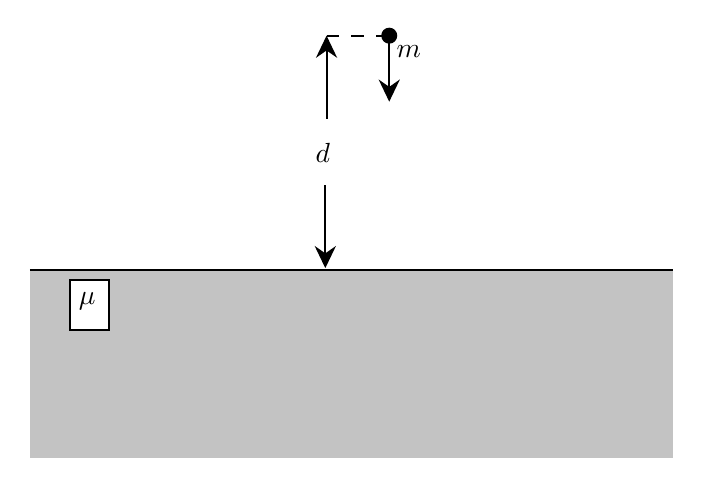
\begin{tikzpicture}[x=0.75pt,y=0.75pt,yscale=-1,xscale=1]
%uncomment if require: \path (0,480); %set diagram left start at 0, and has height of 480

%Shape: Rectangle [id:dp4898925282872699] 
\draw  [draw opacity=0][fill={rgb, 255:red, 155; green, 155; blue, 155 }  ,fill opacity=0.6 ][line width=1.5]  (147.8,233.2) -- (457.8,233.2) -- (457.8,323.46) -- (147.8,323.46) -- cycle ;
%Straight Lines [id:da18901374139949478] 
\draw    (147.8,233.2) -- (457.8,233.2) ;
%Straight Lines [id:da24976008524172455] 
\draw    (321,120.2) -- (321,149) ;
\draw [shift={(321,152)}, rotate = 270] [fill={rgb, 255:red, 0; green, 0; blue, 0 }  ][line width=0.08]  [draw opacity=0] (10.72,-5.15) -- (0,0) -- (10.72,5.15) -- (7.12,0) -- cycle    ;
\draw [shift={(321,120.2)}, rotate = 90] [color={rgb, 255:red, 0; green, 0; blue, 0 }  ][fill={rgb, 255:red, 0; green, 0; blue, 0 }  ][line width=0.75]      (0, 0) circle [x radius= 3.35, y radius= 3.35]   ;
%Straight Lines [id:da35811940778287843] 
\draw  [dash pattern={on 4.5pt off 4.5pt}]  (290.8,120.2) -- (321,120.2) ;
%Straight Lines [id:da08653872575567734] 
\draw    (290.8,160.2) -- (290.8,123.2) ;
\draw [shift={(290.8,120.2)}, rotate = 450] [fill={rgb, 255:red, 0; green, 0; blue, 0 }  ][line width=0.08]  [draw opacity=0] (10.72,-5.15) -- (0,0) -- (10.72,5.15) -- (7.12,0) -- cycle    ;
%Straight Lines [id:da2852991840403014] 
\draw    (290.2,192.2) -- (290.2,229.2) ;
\draw [shift={(290.2,232.2)}, rotate = 270] [fill={rgb, 255:red, 0; green, 0; blue, 0 }  ][line width=0.08]  [draw opacity=0] (10.72,-5.15) -- (0,0) -- (10.72,5.15) -- (7.12,0) -- cycle    ;


% Text Node
\draw (323,123.6) node [anchor=north west][inner sep=0.75pt]    {$\ot{m}$};
% Text Node
\draw (284,170.4) node [anchor=north west][inner sep=0.75pt]    {$d$};
% Text Node
\draw  [fill={rgb, 255:red, 255; green, 255; blue, 255 }  ,fill opacity=1 ]  (167,238) -- (186,238) -- (186,262) -- (167,262) -- cycle  ;
\draw (170,242.4) node [anchor=north west][inner sep=0.75pt]    {$\mu $};


\end{tikzpicture}
\end{center}
\begin{enumerate}[1)]
     \item Tính cường độ từ trường $B$ ở những điểm nằm trong môi trường điện thẩm.
     \item Tính lực tác dụng lên lưỡng cực.
\end{enumerate}
\end{vd}
\begin{loigiai}
    \begin{enumerate}[1)]
      \item Chúng ta sẽ dùng phương pháp ảnh từ để giải quyết bài toán này. Đặt thêm một lưỡng cực từ $\ot{m'}= \alpha \ot{m}$ ở điểm $O'$, đối xứng với lưỡng cực $\ot{m}$ qua bề mặt phân cách của hai môi trường (xem hình vẽ). Từ trường ở vùng $1$ sẽ được tính toán như một tổng của từ trường do $\ot{m}$ và $\ot{m'}$ gây ra. Để tính từ trường ở vùng $2$, chúng ta phải đặt thêm một lưỡng cực khác $\ot{m''}=\beta \ot{m}$ trùng với $\ot{m}$ tại điểm $O$. Chúng ta viết từ trường dưới dạng
  $$\ot{B}^{(1)} = \ot{H}^{(1)} = \frac{3(\ot{m}\cdot \ot{n})\ot{n} - \ot{m}}{r^3} +\alpha \frac{3(\ot{m}\cdot \ot{n'})\ot{n'} -\ot{m}}{r'^3},$$
    $$\ot{H}^{(2)} =\beta \frac{3(\ot{m}\cdot\ot{n})\ot{n} -\ot{m}}{r^3},$$
ở đây $\ot{n},\ot{n'}$ lần lượt là vector đơn vị của $\ot{r},\ot{r'}$ và chỉ số $1$ và $2$ tương ứng với môi trường $1$ và $2$. Như mọi khi, ta viết các điều kiện biên
  \begin{center}
\tikzset{every picture/.style={line width=0.75pt}} %set default line width to 0.75pt        

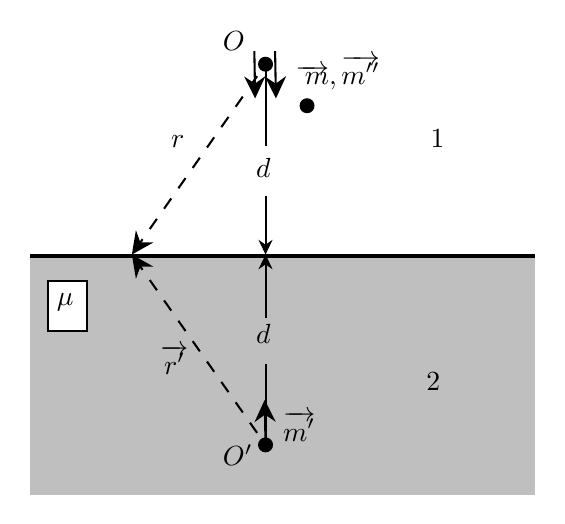
\begin{tikzpicture}[x=0.75pt,y=0.75pt,yscale=-1,xscale=1]
%uncomment if require: \path (0,464); %set diagram left start at 0, and has height of 464

%Shape: Rectangle [id:dp356746186091933] 
\draw  [draw opacity=0][fill={rgb, 255:red, 155; green, 155; blue, 155 }  ,fill opacity=0.64 ] (171.4,277) -- (414.6,277) -- (414.6,392) -- (171.4,392) -- cycle ;
%Straight Lines [id:da9149367444729772] 
\draw [line width=1.5]    (171.4,277) -- (414.6,277) ;
%Straight Lines [id:da9188945714086609] 
\draw    (279.6,178.2) -- (279.95,198) ;
\draw [shift={(280,201)}, rotate = 268.99] [fill={rgb, 255:red, 0; green, 0; blue, 0 }  ][line width=0.08]  [draw opacity=0] (10.72,-5.15) -- (0,0) -- (10.72,5.15) -- (7.12,0) -- cycle    ;
%Straight Lines [id:da4116501102180459] 
\draw    (289.6,178.2) -- (289.95,198) ;
\draw [shift={(290,201)}, rotate = 268.99] [fill={rgb, 255:red, 0; green, 0; blue, 0 }  ][line width=0.08]  [draw opacity=0] (10.72,-5.15) -- (0,0) -- (10.72,5.15) -- (7.12,0) -- cycle    ;
%Shape: Circle [id:dp7919794660449622] 
\draw  [fill={rgb, 255:red, 0; green, 0; blue, 0 }  ,fill opacity=1 ] (281.9,184.5) .. controls (281.9,182.79) and (283.29,181.4) .. (285,181.4) .. controls (286.71,181.4) and (288.1,182.79) .. (288.1,184.5) .. controls (288.1,186.21) and (286.71,187.6) .. (285,187.6) .. controls (283.29,187.6) and (281.9,186.21) .. (281.9,184.5) -- cycle ;
%Straight Lines [id:da399349185589259] 
\draw    (285,184.5) -- (285,273.2) ;
\draw [shift={(285,276.2)}, rotate = 270] [fill={rgb, 255:red, 0; green, 0; blue, 0 }  ][line width=0.08]  [draw opacity=0] (7.14,-3.43) -- (0,0) -- (7.14,3.43) -- (4.74,0) -- cycle    ;
%Straight Lines [id:da13984150406102702] 
\draw    (285,279.2) -- (285,307) ;
\draw [shift={(285,276.2)}, rotate = 90] [fill={rgb, 255:red, 0; green, 0; blue, 0 }  ][line width=0.08]  [draw opacity=0] (7.14,-3.43) -- (0,0) -- (7.14,3.43) -- (4.74,0) -- cycle    ;
%Straight Lines [id:da8974295408894131] 
\draw  [dash pattern={on 4.5pt off 4.5pt}]  (222.32,273.74) -- (285,184.5) ;
\draw [shift={(220.6,276.2)}, rotate = 305.08] [fill={rgb, 255:red, 0; green, 0; blue, 0 }  ][line width=0.08]  [draw opacity=0] (10.72,-5.15) -- (0,0) -- (10.72,5.15) -- (7.12,0) -- cycle    ;
%Straight Lines [id:da24795460376622214] 
\draw  [dash pattern={on 4.5pt off 4.5pt}]  (222.32,278.66) -- (285,367.9) ;
\draw [shift={(220.6,276.2)}, rotate = 54.92] [fill={rgb, 255:red, 0; green, 0; blue, 0 }  ][line width=0.08]  [draw opacity=0] (10.72,-5.15) -- (0,0) -- (10.72,5.15) -- (7.12,0) -- cycle    ;
%Straight Lines [id:da13382982859687442] 
\draw    (285,367.9) -- (284.66,349.2) ;
\draw [shift={(284.6,346.2)}, rotate = 448.94] [fill={rgb, 255:red, 0; green, 0; blue, 0 }  ][line width=0.08]  [draw opacity=0] (10.72,-5.15) -- (0,0) -- (10.72,5.15) -- (7.12,0) -- cycle    ;
%Shape: Circle [id:dp4219420483554077] 
\draw  [fill={rgb, 255:red, 0; green, 0; blue, 0 }  ,fill opacity=1 ] (301.9,204.5) .. controls (301.9,202.79) and (303.29,201.4) .. (305,201.4) .. controls (306.71,201.4) and (308.1,202.79) .. (308.1,204.5) .. controls (308.1,206.21) and (306.71,207.6) .. (305,207.6) .. controls (303.29,207.6) and (301.9,206.21) .. (301.9,204.5) -- cycle ;
%Shape: Circle [id:dp34427786916137393] 
\draw  [fill={rgb, 255:red, 0; green, 0; blue, 0 }  ,fill opacity=1 ] (281.9,367.9) .. controls (281.9,366.19) and (283.29,364.8) .. (285,364.8) .. controls (286.71,364.8) and (288.1,366.19) .. (288.1,367.9) .. controls (288.1,369.61) and (286.71,371) .. (285,371) .. controls (283.29,371) and (281.9,369.61) .. (281.9,367.9) -- cycle ;
%Straight Lines [id:da5759242359947869] 
\draw    (285,329) -- (285,367.9) ;


% Text Node
\draw (298,178.6) node [anchor=north west][inner sep=0.75pt]    {$\overrightarrow{\ m} ,\overrightarrow{m''}$};
% Text Node
\draw (292,350.4) node [anchor=north west][inner sep=0.75pt]    {$\overrightarrow{m'}$};
% Text Node
\draw  [draw opacity=0][fill={rgb, 255:red, 255; green, 255; blue, 255 }  ,fill opacity=1 ]  (276,224) -- (295,224) -- (295,248) -- (276,248) -- cycle  ;
\draw (279,228.4) node [anchor=north west][inner sep=0.75pt]    {$d$};
% Text Node
\draw (279,308.4) node [anchor=north west][inner sep=0.75pt]    {$d$};
% Text Node
\draw (238,217.4) node [anchor=north west][inner sep=0.75pt]    {$\ot{r}$};
% Text Node
\draw (233,318.4) node [anchor=north west][inner sep=0.75pt]    {$\overrightarrow{r'}$};
% Text Node
\draw (363,214.4) node [anchor=north west][inner sep=0.75pt]    {$1$};
% Text Node
\draw (361,331.4) node [anchor=north west][inner sep=0.75pt]    {$2$};
% Text Node
\draw  [fill={rgb, 255:red, 255; green, 255; blue, 255 }  ,fill opacity=1 ]  (180,289) -- (199,289) -- (199,313) -- (180,313) -- cycle  ;
\draw (183,293.4) node [anchor=north west][inner sep=0.75pt]    {$\mu $};
% Text Node
\draw (263,167.4) node [anchor=north west][inner sep=0.75pt]    {$O$};
% Text Node
\draw (263,366.4) node [anchor=north west][inner sep=0.75pt]    {$O'$};


\end{tikzpicture}
\end{center}

ở một điểm $P$ bất kì trên mặt phân cách sao cho $ |\ot{r}| = \abs{\ot{r'}}$
    $$\ot{H_t}^{(1)} = \ot{H_t}^{(2)},$$
$$\ot{B_n}^{(1)} = \ot{B_n}^{(2)} = \mu    \ot{H_n}^{(2)}. $$
Tổng hợp tất cả các phương trình trên ta có
   $$\frac{3m\cos\theta\sin\theta}{r^3} +\alpha \frac{3m\cos\theta\sin\theta}{r^3} =\beta\frac{3m\cos\theta\sin\theta}{r^3},$$
    $$m\frac{3\cos^2 \theta -1}{r^3} - \alpha m\frac{3\cos^2 \theta -1}{r^3} = \mu\beta m \frac{3\cos^2 \theta -1}{r^3}.$$
Từ đó ta rút ra 
    \[\begin{aligned}
     1+\alpha &= \beta,\\
     1- \alpha &= \mu\beta.
    \end{aligned}\]
Dẫn đến
 \[\begin{aligned}
    \beta &= \frac{2}{\mu +1},\\
    \alpha &= 1 -\mu\beta = -\frac{\mu -1}{\mu +1}.
    \end{aligned}\]
Ta kết luận từ trường ở vùng $2$ là
    $$\ot{H}^{(2)} = \frac{2}{\mu +1} \frac{3(\ot{m}\cdot \ot{n})\ot{n} -\ot{m}}{r^3}, \quad\quad \ot{B}^{(2)} =\mu\ot{H}^{(2)} = \frac{2\mu}{\mu +1}\frac{3(\ot{m}\cdot \ot{n})\ot{n} -\ot{m}}{r^3}.$$
\item Lực tác dụng lên lưỡng cực $\ot{m}$ được xác định chỉ bằng từ trường $\ot{B}^{(1)'}$ gây ra bởi lưỡng cực ảnh $\ot{m'}$ trong môi trường $2$ gây ra 
      $$\abs{\ot{F}} = F_x=\ot{m}\cdot\nabla B_x^{(1)'} = -3\frac{2\alpha m^2}{(2d)^4} = \frac{3}{8} \frac{\mu -1}{\mu +1}\frac{m^2}{d^4}.$$
Lưỡng cực bị kéo về phía môi trường điện thẩm. Kết quả cho bài toán tương tự điện từ lưỡng cực  điện đặt trên một mặt phẳng dẫn rộng vô hạn có thể được suy ra bằng cách cho $\mu \rightarrow \infty$
    $$\abs{\ot{F'}} = F'_x = \frac{3}{8} \frac{p^2}{d^4},$$
trong đó $\ot{p}$ là moment lưỡng cực điện.
\end{enumerate}
\end{loigiai}





\begin{vd}[Điện tích và điện môi(G)]
Một điện tích điểm $e$ được đặt tại vị trí $x=h>0,$ $y=z=0$ bên ngoài một khối điện môi đẳng hướng. Khối điện môi chiếm toàn bộ vùng không gian $x<0$ (xem hình vẽ).
   \begin{center}


\tikzset{every picture/.style={line width=0.75pt}} %set default line width to 0.75pt        

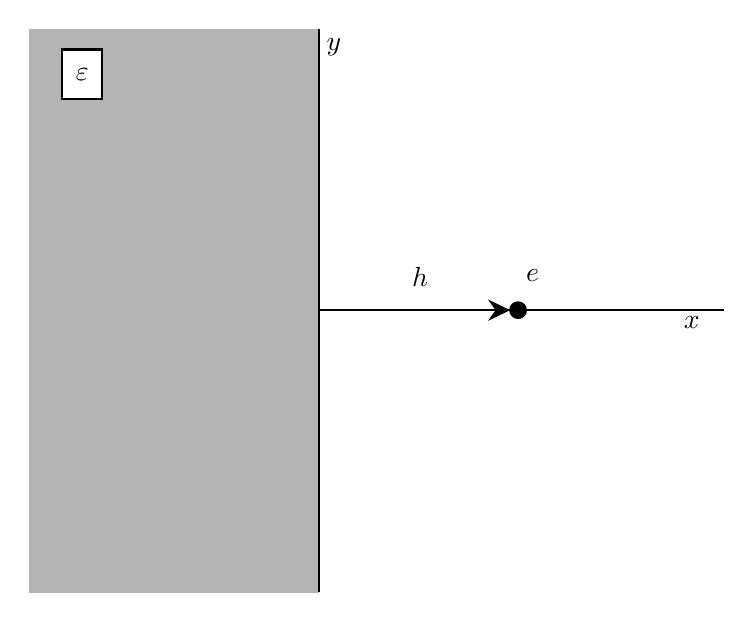
\begin{tikzpicture}[x=0.75pt,y=0.75pt,yscale=-1,xscale=1]
%uncomment if require: \path (0,432); %set diagram left start at 0, and has height of 432

%Shape: Rectangle [id:dp8845109003353693] 
\draw  [draw opacity=0][fill={rgb, 255:red, 155; green, 155; blue, 155 }  ,fill opacity=0.75 ] (127.8,81) -- (267.8,81) -- (267.8,353) -- (127.8,353) -- cycle ;
%Straight Lines [id:da24325499052253874] 
\draw    (267.8,81) -- (267.8,352.2) ;
%Straight Lines [id:da26052780384480045] 
\draw    (267.8,216.6) -- (462.8,216.6) ;
%Shape: Circle [id:dp7016848099113224] 
\draw  [fill={rgb, 255:red, 0; green, 0; blue, 0 }  ,fill opacity=1 ] (367.35,216.6) .. controls (367.35,214.52) and (365.66,212.83) .. (363.57,212.83) .. controls (361.49,212.83) and (359.8,214.52) .. (359.8,216.6) .. controls (359.8,218.68) and (361.49,220.37) .. (363.57,220.37) .. controls (365.66,220.37) and (367.35,218.68) .. (367.35,216.6) -- cycle ;
%Straight Lines [id:da019701475327010387] 
\draw    (267.8,216.6) -- (356.8,216.6) ;
\draw [shift={(359.8,216.6)}, rotate = 180] [fill={rgb, 255:red, 0; green, 0; blue, 0 }  ][line width=0.08]  [draw opacity=0] (10.72,-5.15) -- (0,0) -- (10.72,5.15) -- (7.12,0) -- cycle    ;



% Text Node
\draw (269.8,84.4) node [anchor=north west][inner sep=0.75pt]    {$y$};
% Text Node
\draw (442,218.4) node [anchor=north west][inner sep=0.75pt]    {$x$};
% Text Node
\draw (311,194.4) node [anchor=north west][inner sep=0.75pt]    {$h$};
% Text Node
\draw (366,195.4) node [anchor=north west][inner sep=0.75pt]    {$e$};
% Text Node
\draw  [fill={rgb, 255:red, 255; green, 255; blue, 255 }  ,fill opacity=1 ]  (144,91) -- (163,91) -- (163,115) -- (144,115) -- cycle  ;
\draw (149,98.9) node [anchor=north west][inner sep=0.75pt]    {$\varepsilon $};


\end{tikzpicture}
\end{center}
\begin{enumerate}[1)]
\item Viết biểu thức điện trường $\ot{E} (0^+,y,z)$ và $\ot{E}(0^-,y,z)$ ở điểm ngay phía bên ngoài và điểm ngay phía bên trong vùng điện môi theo điện tích $e$ và mật độ điện tích bề mặt $\sigma_b$ của điện tích hưởng ứng trên bề mặt tấm điện môi.
\item Viết $\sigma_b$ theo $\ot{E}(0^-,y,z)$. Đặt $\varepsilon$ là hằng số điện môi của môi trường bên trong. 
\item Bằng cách sử dụng các phương trình thu được ở $1)$ và $2)$, chứng minh rằng
   $$\sigma_b = -\frac{1}{2\pi} \frac{\varepsilon -1}{\varepsilon +1} \frac {eh}{(h^2 + y^2 + z^2)^{3/2}}.$$ 
\item Tính điện trường $\ot{E'}$ do $\sigma_b$ gây ra tại điểm $(h,0,0)$ của điện tích điểm $e$. Chứng minh rằng điện trường này tương tự điện trường do một điện tích ảnh $e'$ đặt tại điểm $(-h,0,0)$ gây ra.
\item Chứng minh rằng điện tích điểm $e$ chịu một lực bằng
     $$\ot{F} = -\frac{\varepsilon -1}{\varepsilon +1} \frac{e^2}{4h^2}{\hat{x}}.$$
\end{enumerate}
\end{vd}
 \begin{loigiai}
\begin{enumerate}[1)]
   \item Cường độ điện trường ngay trên và ngay dưới vùng điện môi phụ thuộc vào điện tích $e$ và mật độ điện tích mặt $\sigma_b (y,z)$ theo biểu thức
       $$\ot{E}\left(0^{+}, y, z\right)=\frac{e(-h. \hat{{x}}+y .\hat{{y}}+z. \hat{{z}})}{\left(h^{2}+y^{2}+z^{2}\right)^{3 / 2}}+2 \pi \sigma_{b} \hat{{x}},$$
      $$\ot{E}\left(0^{-}, y, z\right)=\frac{e(-h .\hat{{x}}+y. \hat{y}+z. \hat{{z}})}{\left(h^{2}+y^{2}+z^{2}\right)^{3 / 2}}-2 \pi \sigma_{b} \hat{{x}}.$$
  \item Từ công thức $\ot{D} = \ot{E} + 4\pi \ot{P} = \varepsilon \ot{E}$, chúng ta rút ra vector mật độ phân cực $\ot{P}$ và thành phần thẳng đứng $P_n$ của nó tại mặt biên
  \[\begin{aligned}
      \ot{P} &= \frac{\varepsilon -1 }{4\pi} \ot{E},\\
      \sigma_b &= P_n = \frac{\varepsilon -1}{4\pi}E_x (0^-,y,z).
  \end{aligned}\]
  \item Kết hợp các phương trình trên, ta thu được
   $$\sigma_b = \frac{\varepsilon -1}{4\pi} \left[-\frac{eh}{(h^2+y^2+z^2)^{3/2}} -2\pi \sigma_b \right].$$
Do đó
   $$\sigma_b= -\frac{1}{2\pi}\frac{\varepsilon -1}{\varepsilon +1} \frac{eh}{(h^2+y^2+z^2)^{3/2}}.$$
\item Cường độ điện trường tại vị trí điện tích $e$ do điện tích bề mặt $\sigma_b$ gây ra là
    $$\ot{E^{\prime}}(h, 0,0)=\int \frac{h \sigma_{b} \dd A}{\left(h^{2}+y^{2}+z^{2}\right)^{3 / 2}} \hat{{x}},$$
trong đó $\dd\ot{A}$ là vi phân diện tích. Chúng ta chuyển tích phân này sang hệ tọa độ trụ:
   $$\ot{E^{\prime}}(h, 0,0)=-\frac{e}{2 \pi} \frac{\varepsilon-1}{\varepsilon+1} \int_{0}^{2 \pi} \dd \varphi \int_{0}^{\infty} \frac{h^{2} \rho \dd \rho}{\left(h^{2}+\rho^{2}\right)^{3}} \hat{{x}}$$
    $$=-\frac{e}{2} \frac{\varepsilon-1}{\varepsilon+1} \int_{0}^{\infty} \frac{h^{2} \dd \xi \hat{{x}}}{\left(h^{2}+\xi\right)^{3}}=+\left.\frac{e}{4} \frac{\varepsilon-1}{\varepsilon+1} \frac{h^{2}}{\left(h^{2}+\xi\right)^{2}}\right|_{0} ^{\infty} \hat{{x}}=-\frac{\varepsilon-1}{\varepsilon+1} \frac{e}{(2 h)^{2}} \hat{{x}}.$$
Điện trường này tương tự với một điện tích ảnh 
    $$ e' = - \frac{\varepsilon-1}{\varepsilon +1}e$$
đặt ở khoảng cách $2h$ so với điện tích $e$ (xem hình vẽ).
    \begin{center}


\tikzset{every picture/.style={line width=0.75pt}} %set default line width to 0.75pt        

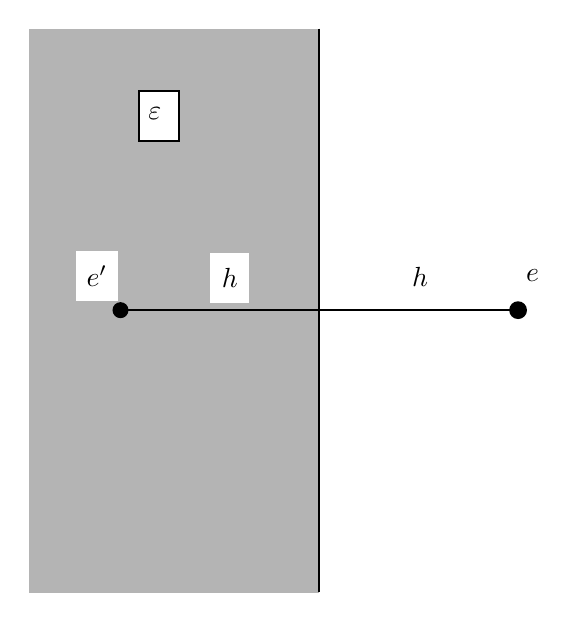
\begin{tikzpicture}[x=0.75pt,y=0.75pt,yscale=-1,xscale=1]
%uncomment if require: \path (0,432); %set diagram left start at 0, and has height of 432

%Shape: Rectangle [id:dp40129217984343746] 
\draw  [draw opacity=0][fill={rgb, 255:red, 155; green, 155; blue, 155 }  ,fill opacity=0.75 ] (124.8,83) -- (264.8,83) -- (264.8,355) -- (124.8,355) -- cycle ;
%Straight Lines [id:da9414478937957673] 
\draw    (264.8,83) -- (264.8,354.2) ;
%Straight Lines [id:da5591796751241624] 
\draw    (264.8,218.6) -- (360.57,218.6) ;
%Shape: Circle [id:dp031766111971942124] 
\draw  [fill={rgb, 255:red, 0; green, 0; blue, 0 }  ,fill opacity=1 ] (364.35,218.6) .. controls (364.35,216.52) and (362.66,214.83) .. (360.57,214.83) .. controls (358.49,214.83) and (356.8,216.52) .. (356.8,218.6) .. controls (356.8,220.68) and (358.49,222.37) .. (360.57,222.37) .. controls (362.66,222.37) and (364.35,220.68) .. (364.35,218.6) -- cycle ;
%Straight Lines [id:da29582843777574475] 
\draw    (169.02,218.6) -- (264.8,218.6) ;
\draw [shift={(169.02,218.6)}, rotate = 0] [color={rgb, 255:red, 0; green, 0; blue, 0 }  ][fill={rgb, 255:red, 0; green, 0; blue, 0 }  ][line width=0.75]      (0, 0) circle [x radius= 3.35, y radius= 3.35]   ;


% Text Node
\draw  [fill={rgb, 255:red, 255; green, 255; blue, 255 }  ,fill opacity=1 ]  (178,113) -- (197,113) -- (197,137) -- (178,137) -- cycle  ;
\draw (181,119.7) node [anchor=north west][inner sep=0.75pt]    {$\varepsilon $};
% Text Node
\draw (308,196.4) node [anchor=north west][inner sep=0.75pt]    {$h$};
% Text Node
\draw (363,197.4) node [anchor=north west][inner sep=0.75pt]    {$e$};
% Text Node
\draw  [draw opacity=0][fill={rgb, 255:red, 255; green, 255; blue, 255 }  ,fill opacity=1 ]  (147.66,190) -- (167.66,190) -- (167.66,214) -- (147.66,214) -- cycle  ;
\draw (157.66,202) node    {$e'$};
% Text Node
\draw  [draw opacity=0][fill={rgb, 255:red, 255; green, 255; blue, 255 }  ,fill opacity=1 ]  (212.16,191) -- (231.16,191) -- (231.16,215) -- (212.16,215) -- cycle  ;
\draw (221.66,203) node    {$h$};


\end{tikzpicture}
\end{center}
\item Lực tác dụng vào điện tích $e$ là
    $$\ot{F} = q\ot{E'} (h,0,0) = -\frac{\varepsilon -1}{\varepsilon +1} \frac{e^2}{4h^2}{\hat{x}}.$$
\end{enumerate}
\end{loigiai}

\begin{vd}[Chất lỏng từ thủy động]%vatdan-dm(1)
\begin{center}
    % Pattern Info
 
\tikzset{
pattern size/.store in=\mcSize, 
pattern size = 5pt,
pattern thickness/.store in=\mcThickness, 
pattern thickness = 0.3pt,
pattern radius/.store in=\mcRadius, 
pattern radius = 1pt}
\makeatletter
\pgfutil@ifundefined{pgf@pattern@name@_sb3w6j11s}{
\pgfdeclarepatternformonly[\mcThickness,\mcSize]{_sb3w6j11s}
{\pgfqpoint{-\mcThickness}{-\mcThickness}}
{\pgfpoint{\mcSize}{\mcSize}}
{\pgfpoint{\mcSize}{\mcSize}}
{
\pgfsetcolor{\tikz@pattern@color}
\pgfsetlinewidth{\mcThickness}
\pgfpathmoveto{\pgfpointorigin}
\pgfpathlineto{\pgfpoint{0}{\mcSize}}
\pgfusepath{stroke}
}}
\makeatother
\tikzset{every picture/.style={line width=0.75pt}} %set default line width to 0.75pt        

\begin{tikzpicture}[x=0.75pt,y=0.75pt,yscale=-1,xscale=1]
%uncomment if require: \path (0,300); %set diagram left start at 0, and has height of 300

%Shape: Rectangle [id:dp7720980006128269] 
\draw  [pattern=_sb3w6j11s,pattern size=6pt,pattern thickness=0.75pt,pattern radius=0pt, pattern color={rgb, 255:red, 155; green, 155; blue, 155}] (150,110.33) -- (481,110.33) -- (481,229.33) -- (150,229.33) -- cycle ;
%Shape: Rectangle [id:dp12408542436065373] 
\draw  [fill={rgb, 255:red, 155; green, 155; blue, 155 }  ,fill opacity=1 ] (111,89.33) -- (521,89.33) -- (521,110) -- (111,110) -- cycle ;
%Shape: Rectangle [id:dp750209091657382] 
\draw  [fill={rgb, 255:red, 155; green, 155; blue, 155 }  ,fill opacity=1 ] (110,229.33) -- (520,229.33) -- (520,250) -- (110,250) -- cycle ;

% Text Node
\draw (274,69) node [anchor=north west][inner sep=0.75pt]   [align=left] {Tấm dẫn};
% Text Node
\draw (279,256) node [anchor=north west][inner sep=0.75pt]   [align=left] {Tấm dẫn};
% Text Node
\draw (261,154) node [anchor=north west][inner sep=0.75pt]   [align=left] {Chất lỏng ER};


\end{tikzpicture}

\end{center}
Chất lỏng từ thủy động (Electrorheological $-$ ER), có cấu tạo từ các quả cầu điện môi nhỏ lơ lửng trong một chất lỏng cách điện, chẳng hạn như dầu silicone, là loại vật liệu có thể chuyển đổi từ trạng thái lỏng sang trạng thái rắn dưới tác dụng của một điện trường bên ngoài. Một thử nghiệm điển hình thiết lập của chất lỏng ER được biểu diễn như hình vẽ, ở đây chất lỏng ER được làm đầy giữa hai tấm dẫn song song có diện tích $A$, khoảng cách giữa hai tấm là $D$. Khi không có điện áp giữa hai tấm, chất lỏng ER ở dạng lỏng do đó các tấm có thể chuyển động theo phương ngang hầu như không có ma sát. Khi một điện áp $V$ được đặt vào giữa hai tấm, các quả cầu nhỏ bị phân cực theo chiều dọc và liên kết thành cột, và để di chuyển tấm dẫn điện tương đối so với tấm kia một độ dịch chuyển nhỏ $\delta x$ đòi hỏi một lực nhỏ $\delta f$. Module cắt $\eta$ được xác định bởi $\eta=\dfrac{D}{A}\dfrac{\delta f}{\delta x}$. Bán kính của quả cầu là $R(\ll D)$, hằng số điện môi của chúng là $\varepsilon$, và tỉ số thể tích của các quả cầu với chất lỏng là $m$. Hằng số điện môi của chất lỏng mà không có các quả cầu $1$. Bỏ qua lực hấp dẫn. Bạn tìm $\eta$ theo những đại lượng vật lý đã cho ở trên.
\begin{center}
    % Gradient Info
  
\tikzset {_jw0nb9tco/.code = {\pgfsetadditionalshadetransform{ \pgftransformshift{\pgfpoint{89.1 bp } { -108.9 bp }  }  \pgftransformscale{1.32 }  }}}
\pgfdeclareradialshading{_b62taj5ms}{\pgfpoint{-72bp}{88bp}}{rgb(0bp)=(1,1,1);
rgb(0.35714285714285715bp)=(1,1,1);
rgb(23.482142857142858bp)=(0,0,0);
rgb(400bp)=(0,0,0)}
\tikzset{every picture/.style={line width=0.75pt}} %set default line width to 0.75pt        

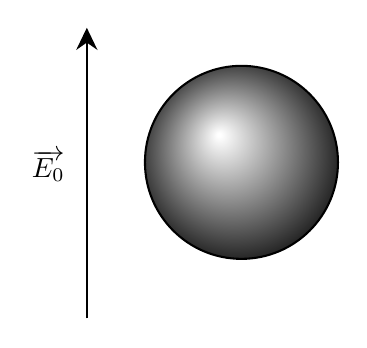
\begin{tikzpicture}[x=0.75pt,y=0.75pt,yscale=-1,xscale=1]
%uncomment if require: \path (0,300); %set diagram left start at 0, and has height of 300

%Shape: Circle [id:dp4353161800756056] 
\path  [shading=_b62taj5ms,_jw0nb9tco] (308,145.5) .. controls (308,119.82) and (328.82,99) .. (354.5,99) .. controls (380.18,99) and (401,119.82) .. (401,145.5) .. controls (401,171.18) and (380.18,192) .. (354.5,192) .. controls (328.82,192) and (308,171.18) .. (308,145.5) -- cycle ; % for fading 
 \draw   (308,145.5) .. controls (308,119.82) and (328.82,99) .. (354.5,99) .. controls (380.18,99) and (401,119.82) .. (401,145.5) .. controls (401,171.18) and (380.18,192) .. (354.5,192) .. controls (328.82,192) and (308,171.18) .. (308,145.5) -- cycle ; % for border 

%Straight Lines [id:da6222153563172375] 
\draw    (280,220.67) -- (280,83.67) ;
\draw [shift={(280,80.67)}, rotate = 450] [fill={rgb, 255:red, 0; green, 0; blue, 0 }  ][line width=0.08]  [draw opacity=0] (10.72,-5.15) -- (0,0) -- (10.72,5.15) -- (7.12,0) -- cycle    ;

% Text Node
\draw (252,138.4) node [anchor=north west][inner sep=0.75pt]    {$\overrightarrow{E_{0}}$};


\end{tikzpicture}

\end{center}
\begin{enumerate}[1)]
    \item Bước đầu tiên là để tìm độ phân cực $\ot{P}$ của một quả cầu cô lập trong một điện trường đều bên ngoài $\ot{E_0}$. Điều này có thể được thực hiện bằng cách giải các ý từ $(a)$ đến $(c)$ dưới đây, và sử dụng một thực tế đã được biết trong điều kiện như vậy sự phân cực là đều trong quả cầu và song song với $\ot{E_0}$.
    \begin{enumerate}[a)]
        \item Tìm điện trường do độ phân cực $\ot{P}$ gây ra ở tâm của quả cầu.
        \item Tìm điện trường tổng hợp bên trong quả cầu.
        \item Moment lưỡng cực điện cảm ứng toàn phần của một quả cầu được viết dưới dạng $\ot{p_0}=\alpha \ot{E_0}$. Tìm hằng số $\alpha$.
    \end{enumerate}
    \item Coi mỗi quả cầu như là một lưỡng cực điện lý tưởng nằm ở tâm của quả cầu, và moment lưỡng cực chỉ phụ thuộc vào $\ot{E_0}$. Nếu bạn chưa tìm thấy $\alpha$ trong ý $(1.c)$, bạn có thể sử dụng nó như một hằng số đã biết để giải quyết các vấn đề sau đây.\\ 
    (\textbf{Gợi ý:} Giữ các số hạng khai triển tới $d^2$, trong đó $d$ là chiều dài của lưỡng cực).
    \begin{enumerate}[a)]
        \item Tìm năng lượng tĩnh điện của hai quả cầu tiếp xúc theo kiểu sát bên cạnh nhau và kiểu trên $-$ dưới, như hình $(2a)$ dưới đây.
        \item Tìm lực tĩnh điện của tấm dẫn lên quả cầu khi quả cầu tiếp xúc với tấm dẫn như hình $(2b)$.
        \item Tìm lực hồi phục theo phương ngang giữa hai quả cầu khi quả cầu bên trên trong kiểu trên $-$ dưới bị dịch chuyển theo phương ngang một đoạn nhỏ $\delta a$ như hình $(2c)$.
    \end{enumerate}
    \end{enumerate}
\begin{center}
    


\tikzset{every picture/.style={line width=0.75pt}} %set default line width to 0.75pt        

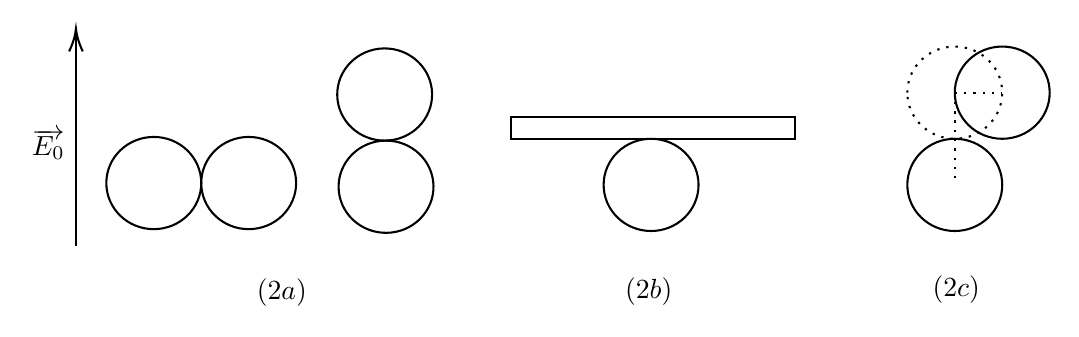
\begin{tikzpicture}[x=0.75pt,y=0.75pt,yscale=-1,xscale=1]
%uncomment if require: \path (0,300); %set diagram left start at 0, and has height of 300

%Straight Lines [id:da7876275917991666] 
\draw    (22.86,202.19) -- (22.86,99.33) ;
\draw [shift={(22.86,97.33)}, rotate = 450] [color={rgb, 255:red, 0; green, 0; blue, 0 }  ][line width=0.75]    (10.93,-3.29) .. controls (6.95,-1.4) and (3.31,-0.3) .. (0,0) .. controls (3.31,0.3) and (6.95,1.4) .. (10.93,3.29)   ;
%Shape: Ellipse [id:dp6145740253615255] 
\draw   (37.49,171.68) .. controls (37.49,159.41) and (47.73,149.47) .. (60.36,149.47) .. controls (72.98,149.47) and (83.22,159.41) .. (83.22,171.68) .. controls (83.22,183.95) and (72.98,193.9) .. (60.36,193.9) .. controls (47.73,193.9) and (37.49,183.95) .. (37.49,171.68) -- cycle ;
%Shape: Ellipse [id:dp948460434401531] 
\draw   (83.22,171.68) .. controls (83.22,159.41) and (93.46,149.47) .. (106.08,149.47) .. controls (118.71,149.47) and (128.94,159.41) .. (128.94,171.68) .. controls (128.94,183.95) and (118.71,193.9) .. (106.08,193.9) .. controls (93.46,193.9) and (83.22,183.95) .. (83.22,171.68) -- cycle ;

%Shape: Ellipse [id:dp8677698449545432] 
\draw   (171.26,106.82) .. controls (183.89,106.64) and (194.27,116.44) .. (194.45,128.71) .. controls (194.63,140.98) and (184.55,151.06) .. (171.92,151.24) .. controls (159.3,151.42) and (148.92,141.62) .. (148.74,129.35) .. controls (148.55,117.09) and (158.64,107) .. (171.26,106.82) -- cycle ;
%Shape: Ellipse [id:dp9885353952628644] 
\draw   (171.93,151.25) .. controls (184.55,151.07) and (194.93,160.87) .. (195.12,173.14) .. controls (195.3,185.4) and (185.21,195.49) .. (172.59,195.67) .. controls (159.96,195.85) and (149.58,186.05) .. (149.4,173.78) .. controls (149.22,161.51) and (159.3,151.42) .. (171.93,151.25) -- cycle ;

%Shape: Ellipse [id:dp7689007820834415] 
\draw   (277.09,172.57) .. controls (277.09,160.3) and (287.33,150.36) .. (299.96,150.36) .. controls (312.58,150.36) and (322.82,160.3) .. (322.82,172.57) .. controls (322.82,184.84) and (312.58,194.79) .. (299.96,194.79) .. controls (287.33,194.79) and (277.09,184.84) .. (277.09,172.57) -- cycle ;
%Shape: Rectangle [id:dp857509416140726] 
\draw   (232.28,139.69) -- (369.46,139.69) -- (369.46,150.36) -- (232.28,150.36) -- cycle ;

%Shape: Ellipse [id:dp5821302713886292] 
\draw   (423.41,172.57) .. controls (423.41,160.3) and (433.65,150.36) .. (446.28,150.36) .. controls (458.9,150.36) and (469.14,160.3) .. (469.14,172.57) .. controls (469.14,184.84) and (458.9,194.79) .. (446.28,194.79) .. controls (433.65,194.79) and (423.41,184.84) .. (423.41,172.57) -- cycle ;
%Shape: Ellipse [id:dp5491352157864255] 
\draw  [dash pattern={on 0.84pt off 2.51pt}] (423.41,128.14) .. controls (423.41,115.87) and (433.65,105.92) .. (446.28,105.92) .. controls (458.9,105.92) and (469.14,115.87) .. (469.14,128.14) .. controls (469.14,140.41) and (458.9,150.36) .. (446.28,150.36) .. controls (433.65,150.36) and (423.41,140.41) .. (423.41,128.14) -- cycle ;
%Shape: Ellipse [id:dp9352354961334186] 
\draw   (446.28,128.14) .. controls (446.28,115.87) and (456.51,105.92) .. (469.14,105.92) .. controls (481.76,105.92) and (492,115.87) .. (492,128.14) .. controls (492,140.41) and (481.76,150.36) .. (469.14,150.36) .. controls (456.51,150.36) and (446.28,140.41) .. (446.28,128.14) -- cycle ;
%Straight Lines [id:da2556120318191424] 
\draw  [dash pattern={on 0.84pt off 2.51pt}]  (446.28,128.14) -- (446.28,172.57) ;
%Straight Lines [id:da08566042590585554] 
\draw  [dash pattern={on 0.84pt off 2.51pt}]  (446.28,128.14) -- (469.14,128.14) ;


% Text Node
\draw (0.1,144.09) node [anchor=north west][inner sep=0.75pt]    {$\overrightarrow{E_{0}}$};
% Text Node
\draw (108.5,216.51) node [anchor=north west][inner sep=0.75pt]    {$(2a)$};
% Text Node
\draw (285.91,215.62) node [anchor=north west][inner sep=0.75pt]    {$(2b)$};
% Text Node
\draw (434.06,214.74) node [anchor=north west][inner sep=0.75pt]    {$(2c)$};


\end{tikzpicture}
\end{center}
\begin{enumerate}[1)]
\setcounter{enumi}{2}
    \item Giả sử dưới tác dụng của điện trường, tất cả các quả cầu được sắp xếp liên tục, thẳng, và có dạng cột mảnh giữa các tấm dẫn. Theo câu trả lời của bạn trong ý $2a$, các cột có giống như là bó với nhau không? Chỉ xét lực giữa các quả cầu kề nhau trong một cột, khi tấm bên trên bị dịch chuyển đi một đoạn nhỏ $\delta x$, quả cầu bên trên của mỗi cột vẫn còn dính vào tấm và được dịch chuyển cùng một khoảng cách với tấm. Như hình vẽ, mỗi quả cầu trong cột dưới đây bị dịch chuyển đều đối với chỉ một quả bên trên. Các quả cầu bên dưới đáy vẫn cố định với tấm bên dưới. Tìm module cắt $\eta$.
\end{enumerate}
\begin{center}
    

\tikzset{every picture/.style={line width=0.75pt}} %set default line width to 0.75pt        

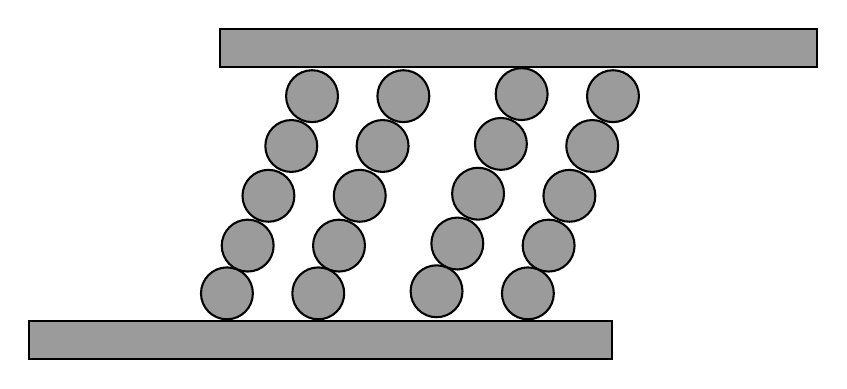
\begin{tikzpicture}[x=0.75pt,y=0.75pt,yscale=-1,xscale=1]
%uncomment if require: \path (0,300); %set diagram left start at 0, and has height of 300

%Shape: Rectangle [id:dp6740434240038389] 
\draw  [fill={rgb, 255:red, 155; green, 155; blue, 155 }  ,fill opacity=1 ] (218,100) -- (506,100) -- (506,118.33) -- (218,118.33) -- cycle ;
%Shape: Rectangle [id:dp9556189737029543] 
\draw  [fill={rgb, 255:red, 155; green, 155; blue, 155 }  ,fill opacity=1 ] (126,241) -- (407,241) -- (407,259.33) -- (126,259.33) -- cycle ;
%Shape: Circle [id:dp7696951200035975] 
\draw  [fill={rgb, 255:red, 155; green, 155; blue, 155 }  ,fill opacity=1 ] (395,132.5) .. controls (395,125.6) and (400.6,120) .. (407.5,120) .. controls (414.4,120) and (420,125.6) .. (420,132.5) .. controls (420,139.4) and (414.4,145) .. (407.5,145) .. controls (400.6,145) and (395,139.4) .. (395,132.5) -- cycle ;
%Shape: Circle [id:dp1308786053146913] 
\draw  [fill={rgb, 255:red, 155; green, 155; blue, 155 }  ,fill opacity=1 ] (385,156.5) .. controls (385,149.6) and (390.6,144) .. (397.5,144) .. controls (404.4,144) and (410,149.6) .. (410,156.5) .. controls (410,163.4) and (404.4,169) .. (397.5,169) .. controls (390.6,169) and (385,163.4) .. (385,156.5) -- cycle ;
%Shape: Circle [id:dp9016028653222721] 
\draw  [fill={rgb, 255:red, 155; green, 155; blue, 155 }  ,fill opacity=1 ] (374,180.5) .. controls (374,173.6) and (379.6,168) .. (386.5,168) .. controls (393.4,168) and (399,173.6) .. (399,180.5) .. controls (399,187.4) and (393.4,193) .. (386.5,193) .. controls (379.6,193) and (374,187.4) .. (374,180.5) -- cycle ;
%Shape: Circle [id:dp1320840002118966] 
\draw  [fill={rgb, 255:red, 155; green, 155; blue, 155 }  ,fill opacity=1 ] (364,204.5) .. controls (364,197.6) and (369.6,192) .. (376.5,192) .. controls (383.4,192) and (389,197.6) .. (389,204.5) .. controls (389,211.4) and (383.4,217) .. (376.5,217) .. controls (369.6,217) and (364,211.4) .. (364,204.5) -- cycle ;
%Shape: Circle [id:dp6050209244676164] 
\draw  [fill={rgb, 255:red, 155; green, 155; blue, 155 }  ,fill opacity=1 ] (354,227.5) .. controls (354,220.6) and (359.6,215) .. (366.5,215) .. controls (373.4,215) and (379,220.6) .. (379,227.5) .. controls (379,234.4) and (373.4,240) .. (366.5,240) .. controls (359.6,240) and (354,234.4) .. (354,227.5) -- cycle ;

%Shape: Circle [id:dp4885252806413358] 
\draw  [fill={rgb, 255:red, 155; green, 155; blue, 155 }  ,fill opacity=1 ] (351,131.5) .. controls (351,124.6) and (356.6,119) .. (363.5,119) .. controls (370.4,119) and (376,124.6) .. (376,131.5) .. controls (376,138.4) and (370.4,144) .. (363.5,144) .. controls (356.6,144) and (351,138.4) .. (351,131.5) -- cycle ;
%Shape: Circle [id:dp7331762405575177] 
\draw  [fill={rgb, 255:red, 155; green, 155; blue, 155 }  ,fill opacity=1 ] (341,155.5) .. controls (341,148.6) and (346.6,143) .. (353.5,143) .. controls (360.4,143) and (366,148.6) .. (366,155.5) .. controls (366,162.4) and (360.4,168) .. (353.5,168) .. controls (346.6,168) and (341,162.4) .. (341,155.5) -- cycle ;
%Shape: Circle [id:dp5912171983599124] 
\draw  [fill={rgb, 255:red, 155; green, 155; blue, 155 }  ,fill opacity=1 ] (330,179.5) .. controls (330,172.6) and (335.6,167) .. (342.5,167) .. controls (349.4,167) and (355,172.6) .. (355,179.5) .. controls (355,186.4) and (349.4,192) .. (342.5,192) .. controls (335.6,192) and (330,186.4) .. (330,179.5) -- cycle ;
%Shape: Circle [id:dp4565422945680693] 
\draw  [fill={rgb, 255:red, 155; green, 155; blue, 155 }  ,fill opacity=1 ] (320,203.5) .. controls (320,196.6) and (325.6,191) .. (332.5,191) .. controls (339.4,191) and (345,196.6) .. (345,203.5) .. controls (345,210.4) and (339.4,216) .. (332.5,216) .. controls (325.6,216) and (320,210.4) .. (320,203.5) -- cycle ;
%Shape: Circle [id:dp12185227717454117] 
\draw  [fill={rgb, 255:red, 155; green, 155; blue, 155 }  ,fill opacity=1 ] (310,226.5) .. controls (310,219.6) and (315.6,214) .. (322.5,214) .. controls (329.4,214) and (335,219.6) .. (335,226.5) .. controls (335,233.4) and (329.4,239) .. (322.5,239) .. controls (315.6,239) and (310,233.4) .. (310,226.5) -- cycle ;

%Shape: Circle [id:dp7263596093938309] 
\draw  [fill={rgb, 255:red, 155; green, 155; blue, 155 }  ,fill opacity=1 ] (294,132.5) .. controls (294,125.6) and (299.6,120) .. (306.5,120) .. controls (313.4,120) and (319,125.6) .. (319,132.5) .. controls (319,139.4) and (313.4,145) .. (306.5,145) .. controls (299.6,145) and (294,139.4) .. (294,132.5) -- cycle ;
%Shape: Circle [id:dp9648642270660002] 
\draw  [fill={rgb, 255:red, 155; green, 155; blue, 155 }  ,fill opacity=1 ] (284,156.5) .. controls (284,149.6) and (289.6,144) .. (296.5,144) .. controls (303.4,144) and (309,149.6) .. (309,156.5) .. controls (309,163.4) and (303.4,169) .. (296.5,169) .. controls (289.6,169) and (284,163.4) .. (284,156.5) -- cycle ;
%Shape: Circle [id:dp1474441789562353] 
\draw  [fill={rgb, 255:red, 155; green, 155; blue, 155 }  ,fill opacity=1 ] (273,180.5) .. controls (273,173.6) and (278.6,168) .. (285.5,168) .. controls (292.4,168) and (298,173.6) .. (298,180.5) .. controls (298,187.4) and (292.4,193) .. (285.5,193) .. controls (278.6,193) and (273,187.4) .. (273,180.5) -- cycle ;
%Shape: Circle [id:dp8535757103166481] 
\draw  [fill={rgb, 255:red, 155; green, 155; blue, 155 }  ,fill opacity=1 ] (263,204.5) .. controls (263,197.6) and (268.6,192) .. (275.5,192) .. controls (282.4,192) and (288,197.6) .. (288,204.5) .. controls (288,211.4) and (282.4,217) .. (275.5,217) .. controls (268.6,217) and (263,211.4) .. (263,204.5) -- cycle ;
%Shape: Circle [id:dp5677990235384391] 
\draw  [fill={rgb, 255:red, 155; green, 155; blue, 155 }  ,fill opacity=1 ] (253,227.5) .. controls (253,220.6) and (258.6,215) .. (265.5,215) .. controls (272.4,215) and (278,220.6) .. (278,227.5) .. controls (278,234.4) and (272.4,240) .. (265.5,240) .. controls (258.6,240) and (253,234.4) .. (253,227.5) -- cycle ;

%Shape: Circle [id:dp9345507138795539] 
\draw  [fill={rgb, 255:red, 155; green, 155; blue, 155 }  ,fill opacity=1 ] (250,132.5) .. controls (250,125.6) and (255.6,120) .. (262.5,120) .. controls (269.4,120) and (275,125.6) .. (275,132.5) .. controls (275,139.4) and (269.4,145) .. (262.5,145) .. controls (255.6,145) and (250,139.4) .. (250,132.5) -- cycle ;
%Shape: Circle [id:dp5225099980893457] 
\draw  [fill={rgb, 255:red, 155; green, 155; blue, 155 }  ,fill opacity=1 ] (240,156.5) .. controls (240,149.6) and (245.6,144) .. (252.5,144) .. controls (259.4,144) and (265,149.6) .. (265,156.5) .. controls (265,163.4) and (259.4,169) .. (252.5,169) .. controls (245.6,169) and (240,163.4) .. (240,156.5) -- cycle ;
%Shape: Circle [id:dp03735737662274863] 
\draw  [fill={rgb, 255:red, 155; green, 155; blue, 155 }  ,fill opacity=1 ] (229,180.5) .. controls (229,173.6) and (234.6,168) .. (241.5,168) .. controls (248.4,168) and (254,173.6) .. (254,180.5) .. controls (254,187.4) and (248.4,193) .. (241.5,193) .. controls (234.6,193) and (229,187.4) .. (229,180.5) -- cycle ;
%Shape: Circle [id:dp8241391622759215] 
\draw  [fill={rgb, 255:red, 155; green, 155; blue, 155 }  ,fill opacity=1 ] (219,204.5) .. controls (219,197.6) and (224.6,192) .. (231.5,192) .. controls (238.4,192) and (244,197.6) .. (244,204.5) .. controls (244,211.4) and (238.4,217) .. (231.5,217) .. controls (224.6,217) and (219,211.4) .. (219,204.5) -- cycle ;
%Shape: Circle [id:dp6010407520064651] 
\draw  [fill={rgb, 255:red, 155; green, 155; blue, 155 }  ,fill opacity=1 ] (209,227.5) .. controls (209,220.6) and (214.6,215) .. (221.5,215) .. controls (228.4,215) and (234,220.6) .. (234,227.5) .. controls (234,234.4) and (228.4,240) .. (221.5,240) .. controls (214.6,240) and (209,234.4) .. (209,227.5) -- cycle ;

\end{tikzpicture}
\end{center}
\end{vd}
\begin{loigiai}
\begin{enumerate}[1)]
    \item 
    \begin{enumerate}[a)]
        \item Mật độ điện tích mặt
        \[\sigma=P\mathrm{\cos{\theta}},\]
         \textbf{Chú ý.} Để lời giải dễ hiểu hơn, chúng tôi bổ sung như sau:\\ Mật độ điện tích mặt tại yếu tố điện tích $\mathrm{d}S=R^2{\sin{\theta}}\mathrm{d}\theta\mathrm{d}\phi$ trên mặt cầu bán kính $R$ là $\sigma=P\cos{\theta}$ với $\theta$ là góc cực, $\phi$ là góc phương vị.\\ Khi đó cường độ điện trường do độ phân cực $\ot{P}$ gây ra ở tâm quả cầu dọc theo trục $z$ của quả cầu là
         \[E_{\mathrm{P}}=\dfrac{P}{4\pi\varepsilon_0R^2}\cdot2\cdot\int_{0}^{\dfrac{\pi}{2}}\mathrm{d}\theta\mathrm{\cos{\theta}}R^2\mathrm{\sin{\theta}}\mathrm{\cos{\theta}}\int_{0}^{2\pi}\mathrm{d}\phi=\dfrac{P}{3\varepsilon_0}.\]
        \begin{center}


\tikzset{every picture/.style={line width=0.75pt}} %set default line width to 0.75pt        

\begin{tikzpicture}[x=0.75pt,y=0.75pt,yscale=-1,xscale=1]
%uncomment if require: \path (0,300); %set diagram left start at 0, and has height of 300

%Shape: Circle [id:dp06806449925848446] 
\draw   (214.67,143.17) .. controls (214.67,83.98) and (262.65,36) .. (321.83,36) .. controls (381.02,36) and (429,83.98) .. (429,143.17) .. controls (429,202.35) and (381.02,250.33) .. (321.83,250.33) .. controls (262.65,250.33) and (214.67,202.35) .. (214.67,143.17) -- cycle ;
%Curve Lines [id:da08107531747917118] 
\draw    (214.67,146.53) .. controls (224,183.33) and (426,181.33) .. (429,146.53) ;
%Curve Lines [id:da26617387968351425] 
\draw  [dash pattern={on 0.84pt off 2.51pt}]  (214.67,146.53) .. controls (226,108.33) and (426,112.33) .. (429,146.53) ;

%Curve Lines [id:da8018712605038762] 
\draw    (242,72.42) .. controls (248.97,88.75) and (399.76,87.86) .. (402,72.42) ;
%Curve Lines [id:da2618039979793949] 
\draw  [dash pattern={on 0.84pt off 2.51pt}]  (242,72.42) .. controls (250.46,55.47) and (399.76,57.24) .. (402,72.42) ;

%Curve Lines [id:da4257978520158401] 
\draw    (321.83,36) .. controls (365,60.67) and (377,217.33) .. (321.83,250.33) ;
%Straight Lines [id:da48105810564830875] 
\draw    (321.83,143.17) -- (495,143.17) ;
\draw [shift={(498,143.17)}, rotate = 180] [fill={rgb, 255:red, 0; green, 0; blue, 0 }  ][line width=0.08]  [draw opacity=0] (10.72,-5.15) -- (0,0) -- (10.72,5.15) -- (7.12,0) -- cycle    ;
%Straight Lines [id:da40628045711216565] 
\draw    (321.83,143.17) -- (321.83,9.67) ;
\draw [shift={(321.83,6.67)}, rotate = 450] [fill={rgb, 255:red, 0; green, 0; blue, 0 }  ][line width=0.08]  [draw opacity=0] (10.72,-5.15) -- (0,0) -- (10.72,5.15) -- (7.12,0) -- cycle    ;
%Straight Lines [id:da1361543172905233] 
\draw    (321.83,143.17) -- (224.12,240.88) ;
\draw [shift={(222,243)}, rotate = 315] [fill={rgb, 255:red, 0; green, 0; blue, 0 }  ][line width=0.08]  [draw opacity=0] (10.72,-5.15) -- (0,0) -- (10.72,5.15) -- (7.12,0) -- cycle    ;
%Straight Lines [id:da91889675049976] 
\draw  [dash pattern={on 0.84pt off 2.51pt}]  (349.42,84.75) -- (349.42,161.33) ;
%Straight Lines [id:da019606924097860468] 
\draw  [dash pattern={on 0.84pt off 2.51pt}]  (349,163.67) -- (293,172.33) ;
%Straight Lines [id:da8632539747166392] 
\draw  [dash pattern={on 0.84pt off 2.51pt}]  (402,143.33) -- (353.47,161.95) -- (349,163.67) ;
%Straight Lines [id:da03900549562044775] 
\draw  [dash pattern={on 0.84pt off 2.51pt}]  (322,60.67) -- (349.42,84.75) ;
%Straight Lines [id:da0319604711486432] 
\draw    (321.83,143.17) -- (377,26.33) ;
%Straight Lines [id:da5646379670921662] 
\draw    (321.83,143.17) -- (348.14,87.46) ;
\draw [shift={(349.42,84.75)}, rotate = 475.28] [fill={rgb, 255:red, 0; green, 0; blue, 0 }  ][line width=0.08]  [draw opacity=0] (10.72,-5.15) -- (0,0) -- (10.72,5.15) -- (7.12,0) -- cycle    ;
%Curve Lines [id:da12043994966366167] 
\draw    (313,151.33) .. controls (318.07,158.09) and (323.85,154.86) .. (328.54,151.88) ;
\draw [shift={(331,150.33)}, rotate = 509.04] [fill={rgb, 255:red, 0; green, 0; blue, 0 }  ][line width=0.08]  [draw opacity=0] (10.72,-5.15) -- (0,0) -- (10.72,5.15) -- (7.12,0) -- cycle    ;
%Straight Lines [id:da8063040078569479] 
\draw  [dash pattern={on 0.84pt off 2.51pt}]  (359,171.33) -- (321.83,143.17) ;
%Curve Lines [id:da200383054065143] 
\draw    (322,105.33) .. controls (325.08,103.79) and (331.12,108.78) .. (334.48,111.89) ;
\draw [shift={(336.63,113.96)}, rotate = 225] [fill={rgb, 255:red, 0; green, 0; blue, 0 }  ][line width=0.08]  [draw opacity=0] (10.72,-5.15) -- (0,0) -- (10.72,5.15) -- (7.12,0) -- cycle    ;
%Straight Lines [id:da16424201018162732] 
\draw    (159,104.67) -- (252.09,81.39) ;
\draw [shift={(255,80.67)}, rotate = 525.96] [fill={rgb, 255:red, 0; green, 0; blue, 0 }  ][line width=0.08]  [draw opacity=0] (10.72,-5.15) -- (0,0) -- (10.72,5.15) -- (7.12,0) -- cycle    ;
%Straight Lines [id:da45583682412366566] 
\draw    (466,225.67) -- (355.92,199.36) ;
\draw [shift={(353,198.67)}, rotate = 373.44] [fill={rgb, 255:red, 0; green, 0; blue, 0 }  ][line width=0.08]  [draw opacity=0] (10.72,-5.15) -- (0,0) -- (10.72,5.15) -- (7.12,0) -- cycle    ;

% Text Node
\draw (300,132.4) node [anchor=north west][inner sep=0.75pt]  [font=\small]  {$O$};
% Text Node
\draw (356,86.4) node [anchor=north west][inner sep=0.75pt]  [font=\small]  {$M$};
% Text Node
\draw (211,219.4) node [anchor=north west][inner sep=0.75pt]  [font=\small]  {$x$};
% Text Node
\draw (498,123.4) node [anchor=north west][inner sep=0.75pt]  [font=\small]  {$y$};
% Text Node
\draw (306,12.4) node [anchor=north west][inner sep=0.75pt]  [font=\small]  {$z$};
% Text Node
\draw (283,161.4) node [anchor=north west][inner sep=0.75pt]  [font=\small]  {$x$};
% Text Node
\draw (401,143.4) node [anchor=north west][inner sep=0.75pt]  [font=\small]  {$y$};
% Text Node
\draw (313,50.4) node [anchor=north west][inner sep=0.75pt]  [font=\small]  {$z$};
% Text Node
\draw (334,120.4) node [anchor=north west][inner sep=0.75pt]  [font=\small]  {$r$};
% Text Node
\draw (379,6.4) node [anchor=north west][inner sep=0.75pt]  [font=\small]  {$\mathrm{d}\overrightarrow{E_{p}}$};
% Text Node
\draw (325,90.4) node [anchor=north west][inner sep=0.75pt]  [font=\footnotesize]  {$\theta $};
% Text Node
\draw (311,155.4) node [anchor=north west][inner sep=0.75pt]  [font=\scriptsize]  {$\varphi $};
% Text Node
\draw (129,105) node [anchor=north west][inner sep=0.75pt]  [font=\small] [align=left] {Vĩ tuyến};
% Text Node
\draw (440,229) node [anchor=north west][inner sep=0.75pt]  [font=\small] [align=left] {Kinh tuyến};


\end{tikzpicture}
        \end{center}
        
        \item Ta có $E=E_{\mathrm{0}}-E_{\mathrm{p}}$ với $E_{\mathrm{p}}=\dfrac{P}{3\varepsilon_0}$ và $P=\varepsilon_0(\varepsilon-1)E=\chi\varepsilon_0E$, suy ra
        \[ E=E_0-\dfrac{P}{3\varepsilon_0}=E_0-\dfrac{\varepsilon-1}{3}E.\]
        Từ đó, ta suy ra
        \[\ot{E}=\dfrac{3}{\varepsilon+2}\ot{E_0}.\]
        \item Ta có
        \begin{align*}
            \ot{P}&=(\varepsilon-1)\varepsilon_0\ot{E}\\
            &=3\varepsilon_0\dfrac{(\varepsilon-1)}{(\varepsilon+2)}\ot{E_0}.\\
            \ot{p}&=\dfrac{4}{3}\pi R^3 \ot{P}=\dfrac{4}{3}\pi R^3\cdot3\varepsilon_0\dfrac{(\varepsilon-1)}{(\varepsilon+2)}\ot{E_0}\\
            &=4\pi R^3 \varepsilon_0 \dfrac{(\varepsilon-1)}{(\varepsilon+2)}\ot{E_0}.
        \end{align*}
        Do đó ta thu được $\alpha=4\pi R^3 \varepsilon_0 \dfrac{(\varepsilon-1)}{(\varepsilon+2)}$.
    \end{enumerate}
    \item 
    \begin{enumerate}[a)]
        \item
        \begin{align*}
        W&=\dfrac{2Q^2}{4\pi\varepsilon_0}\left(\dfrac{1}{2R}-\dfrac{1}{\sqrt{4R^2+d^2}}\right)=\dfrac{p^2}{32\pi\varepsilon_0R^3}.\\
        W&=-\dfrac{p^2}{16\pi\varepsilon_0R^3} .
        \end{align*}
  
        \item Sử dụng phương pháp ảnh điện 
        \begin{align*}
            W&=\dfrac{p^2}{16\pi\varepsilon_0R^3}.\\
            F&=\dfrac{\partial W}{\partial(2R)}=\dfrac{3p^2}{32\pi\varepsilon_0R^4}.
        \end{align*}
        \item
        \[\dfrac{Q^2}{4\pi\varepsilon_0}\left(\dfrac{2}{\sqrt{4R^2+x^2}}-\dfrac{1}{\sqrt{(2R-d)^2+x^2}}-\dfrac{1}{\sqrt{(2R+d)^2+x^2}}\right)=-\dfrac{3p^2}{128\pi\varepsilon_0R^5}x^2.\]
        Lực cần tìm là
        \[F=-\dfrac{\mathrm{d}W}{\mathrm{d}x}=\dfrac{3p^2}{64\pi\varepsilon_0R^5}\delta x.\]
    \end{enumerate}
    \item Ở bên trái cũng như ở bên phải, năng lượng là dương, và tỉ lệ nghịch với lập phương của khoảng cách, các quả cầu dễ dàng để dính vào nhau.\\
    Thể tích của cột là
    \[\dfrac{4\pi R^3}{3}\cdot\dfrac{D}{2R}.\]
    Tổng thể tích của các quả cầu là $ADm$. Số lượng các cột là
    \[\dfrac{ADm}{\dfrac{4\pi R^3}{3}\cdot\dfrac{D}{2R}}.\]
    Ta có $\delta a=\dfrac{2R}{D}\delta x$ và $\delta f=F$
    Do đó module cắt là
    \[\eta=\dfrac{D\delta f}{A\delta x}=\dfrac{9m\varepsilon_0}{4}\left(\dfrac{\varepsilon-1}{\varepsilon+2}\right)^2\left(\dfrac{V}{D}\right)^2=\dfrac{9m\varepsilon_0}{4}\left(\dfrac{\varepsilon-1}{\varepsilon+2}\right)^2E_0^2.\]

\end{enumerate}
\end{loigiai}

\begin{vd}[Các mặt cầu điện môi]
Không gian giữa hai lớp vật dẫn hình tròn đồng tâm bán kính $R_1$ và $R_3$ được lấp đầy bởi hai loại môi trường. Các hằng số điện môi và độ dẫn điện của môi trường $1$ và môi trường $2$ tương ứng lần lượt là $\varepsilon_1$, $\sigma_1$ và $\varepsilon_2$, $\sigma_2$. Hiệu điện thế giữa hai lớp cầu là $V_0$.
\begin{center}
   

% Pattern Info
 
\tikzset{
pattern size/.store in=\mcSize, 
pattern size = 5pt,
pattern thickness/.store in=\mcThickness, 
pattern thickness = 0.3pt,
pattern radius/.store in=\mcRadius, 
pattern radius = 1pt}
\makeatletter
\pgfutil@ifundefined{pgf@pattern@name@_0wb14mxr3}{
\makeatletter
\pgfdeclarepatternformonly[\mcRadius,\mcThickness,\mcSize]{_0wb14mxr3}
{\pgfpoint{-0.5*\mcSize}{-0.5*\mcSize}}
{\pgfpoint{0.5*\mcSize}{0.5*\mcSize}}
{\pgfpoint{\mcSize}{\mcSize}}
{
\pgfsetcolor{\tikz@pattern@color}
\pgfsetlinewidth{\mcThickness}
\pgfpathcircle\pgfpointorigin{\mcRadius}
\pgfusepath{stroke}
}}
\makeatother

% Pattern Info
 
\tikzset{
pattern size/.store in=\mcSize, 
pattern size = 5pt,
pattern thickness/.store in=\mcThickness, 
pattern thickness = 0.3pt,
pattern radius/.store in=\mcRadius, 
pattern radius = 1pt}
\makeatletter
\pgfutil@ifundefined{pgf@pattern@name@_ix0jxyury}{
\pgfdeclarepatternformonly[\mcThickness,\mcSize]{_ix0jxyury}
{\pgfqpoint{0pt}{0pt}}
{\pgfpoint{\mcSize+\mcThickness}{\mcSize+\mcThickness}}
{\pgfpoint{\mcSize}{\mcSize}}
{
\pgfsetcolor{\tikz@pattern@color}
\pgfsetlinewidth{\mcThickness}
\pgfpathmoveto{\pgfqpoint{0pt}{0pt}}
\pgfpathlineto{\pgfpoint{\mcSize+\mcThickness}{\mcSize+\mcThickness}}
\pgfusepath{stroke}
}}
\makeatother

% Pattern Info
 
\tikzset{
pattern size/.store in=\mcSize, 
pattern size = 5pt,
pattern thickness/.store in=\mcThickness, 
pattern thickness = 0.3pt,
pattern radius/.store in=\mcRadius, 
pattern radius = 1pt}
\makeatletter
\pgfutil@ifundefined{pgf@pattern@name@_ucurboj1z}{
\makeatletter
\pgfdeclarepatternformonly[\mcRadius,\mcThickness,\mcSize]{_ucurboj1z}
{\pgfpoint{-0.5*\mcSize}{-0.5*\mcSize}}
{\pgfpoint{0.5*\mcSize}{0.5*\mcSize}}
{\pgfpoint{\mcSize}{\mcSize}}
{
\pgfsetcolor{\tikz@pattern@color}
\pgfsetlinewidth{\mcThickness}
\pgfpathcircle\pgfpointorigin{\mcRadius}
\pgfusepath{stroke}
}}
\makeatother
\tikzset{every picture/.style={line width=0.75pt}} %set default line width to 0.75pt        

\begin{tikzpicture}[x=0.75pt,y=0.75pt,yscale=-1,xscale=1]
%uncomment if require: \path (0,300); %set diagram left start at 0, and has height of 300

%Shape: Circle [id:dp47140438735985035] 
\draw  [color={rgb, 255:red, 0; green, 0; blue, 0 }  ,draw opacity=1 ][pattern=_0wb14mxr3,pattern size=6pt,pattern thickness=0.75pt,pattern radius=0.75pt, pattern color={rgb, 255:red, 0; green, 0; blue, 0}][line width=1.5]  (76.67,146.17) .. controls (76.67,100.79) and (113.45,64) .. (158.83,64) .. controls (204.21,64) and (241,100.79) .. (241,146.17) .. controls (241,191.55) and (204.21,228.33) .. (158.83,228.33) .. controls (113.45,228.33) and (76.67,191.55) .. (76.67,146.17) -- cycle ;
%Shape: Circle [id:dp41017911721051736] 
\draw  [color={rgb, 255:red, 0; green, 0; blue, 0 }  ,draw opacity=1 ][fill={rgb, 255:red, 155; green, 155; blue, 155 }  ,fill opacity=1 ] (105.96,146.17) .. controls (105.96,116.96) and (129.63,93.29) .. (158.83,93.29) .. controls (188.04,93.29) and (211.71,116.96) .. (211.71,146.17) .. controls (211.71,175.37) and (188.04,199.04) .. (158.83,199.04) .. controls (129.63,199.04) and (105.96,175.37) .. (105.96,146.17) -- cycle ;
%Shape: Circle [id:dp9167132354363448] 
\draw  [fill={rgb, 255:red, 255; green, 255; blue, 255 }  ,fill opacity=0.8 ] (122.83,146.17) .. controls (122.83,126.28) and (138.95,110.17) .. (158.83,110.17) .. controls (178.72,110.17) and (194.83,126.28) .. (194.83,146.17) .. controls (194.83,166.05) and (178.72,182.17) .. (158.83,182.17) .. controls (138.95,182.17) and (122.83,166.05) .. (122.83,146.17) -- cycle ;
%Straight Lines [id:da9017262931356629] 
\draw    (158.83,146.17) -- (191.83,146.17) ;
\draw [shift={(194.83,146.17)}, rotate = 180] [fill={rgb, 255:red, 0; green, 0; blue, 0 }  ][line width=0.08]  [draw opacity=0] (10.72,-5.15) -- (0,0) -- (10.72,5.15) -- (7.12,0) -- cycle    ;
%Straight Lines [id:da496676617935093] 
\draw    (158.83,146.17) -- (158.83,96.29) ;
\draw [shift={(158.83,93.29)}, rotate = 450] [fill={rgb, 255:red, 0; green, 0; blue, 0 }  ][line width=0.08]  [draw opacity=0] (10.72,-5.15) -- (0,0) -- (10.72,5.15) -- (7.12,0) -- cycle    ;
%Straight Lines [id:da906998210471998] 
\draw    (158.83,146.17) -- (211,204.43) ;
\draw [shift={(213,206.67)}, rotate = 228.16] [fill={rgb, 255:red, 0; green, 0; blue, 0 }  ][line width=0.08]  [draw opacity=0] (10.72,-5.15) -- (0,0) -- (10.72,5.15) -- (7.12,0) -- cycle    ;

%Shape: Arc [id:dp23640096903274932] 
\draw  [draw opacity=1][pattern=_ix0jxyury,pattern size=6pt,pattern thickness=0.75pt,pattern radius=0pt, pattern color={rgb, 255:red, 0; green, 0; blue, 0}] (396.51,146.72) .. controls (396.5,146.14) and (396.49,145.57) .. (396.49,144.99) .. controls (396.46,98.33) and (432.69,60.48) .. (477.42,60.45) .. controls (522.14,60.42) and (558.42,98.22) .. (558.46,144.88) .. controls (558.46,145.05) and (558.46,145.21) .. (558.45,145.37) -- (477.47,144.94) -- cycle ; \draw   (396.51,146.72) .. controls (396.5,146.14) and (396.49,145.57) .. (396.49,144.99) .. controls (396.46,98.33) and (432.69,60.48) .. (477.42,60.45) .. controls (522.14,60.42) and (558.42,98.22) .. (558.46,144.88) .. controls (558.46,145.05) and (558.46,145.21) .. (558.45,145.37) ;
%Straight Lines [id:da9380058364999] 
\draw    (558.45,145.4) -- (396.51,146.79) ;
%Shape: Arc [id:dp42376990655914204] 
\draw  [draw opacity=1][pattern=_ucurboj1z,pattern size=6pt,pattern thickness=0.75pt,pattern radius=0.75pt, pattern color={rgb, 255:red, 0; green, 0; blue, 0}] (558.47,145.81) .. controls (558.06,191.38) and (522.95,228.63) .. (478.98,229.5) .. controls (434.44,230.39) and (397.61,193.62) .. (396.41,147.25) -- (477.43,144.97) -- cycle ; \draw   (558.47,145.81) .. controls (558.06,191.38) and (522.95,228.63) .. (478.98,229.5) .. controls (434.44,230.39) and (397.61,193.62) .. (396.41,147.25) ;

%Shape: Circle [id:dp6437675374283061] 
\draw  [fill={rgb, 243:red, 243; green, 243; blue, 243 }  ,fill opacity=1 ][line width=1.5]  (424.48,144.94) .. controls (424.48,115.67) and (448.21,91.94) .. (477.47,91.94) .. controls (506.74,91.94) and (530.47,115.67) .. (530.47,144.94) .. controls (530.47,174.2) and (506.74,197.93) .. (477.47,197.93) .. controls (448.21,197.93) and (424.48,174.2) .. (424.48,144.94) -- cycle ;
%Straight Lines [id:da8201725959353237] 
\draw    (477.47,144.94) -- (515.64,114.86) ;
\draw [shift={(518,113)}, rotate = 501.76] [fill={rgb, 255:red, 0; green, 0; blue, 0 }  ][line width=0.08]  [draw opacity=0] (10.72,-5.15) -- (0,0) -- (10.72,5.15) -- (7.12,0) -- cycle    ;
%Straight Lines [id:da620971908682113] 
\draw    (477.47,144.94) -- (533.87,201.33) ;
\draw [shift={(535.99,203.45)}, rotate = 225] [fill={rgb, 255:red, 0; green, 0; blue, 0 }  ][line width=0.08]  [draw opacity=0] (10.72,-5.15) -- (0,0) -- (10.72,5.15) -- (7.12,0) -- cycle    ;

% Text Node
\draw (423,243) node [anchor=north west][inner sep=0.75pt]   [align=left] {Trường hợp $\displaystyle B$};
% Text Node
\draw (479,115.4) node [anchor=north west][inner sep=0.75pt]  [font=\footnotesize]  {$R_{1}$};
% Text Node
\draw (499,150.4) node [anchor=north west][inner sep=0.75pt]  [font=\footnotesize]  {$R_{3}$};
% Text Node
\draw (478,71.4) node [anchor=north west][inner sep=0.75pt]    {$\mathbf{1}$};
% Text Node
\draw (472,203.4) node [anchor=north west][inner sep=0.75pt]    {$\mathbf{2}$};
% Text Node
\draw (108,239) node [anchor=north west][inner sep=0.75pt]   [align=left] {Trường hợp $\displaystyle A$};
% Text Node
\draw (166,130.4) node [anchor=north west][inner sep=0.75pt]  [font=\footnotesize]  {$R_{1}$};
% Text Node
\draw (139,119.4) node [anchor=north west][inner sep=0.75pt]  [font=\footnotesize]  {$R_{2}$};
% Text Node
\draw (154,158.4) node [anchor=north west][inner sep=0.75pt]  [font=\footnotesize]  {$R_{3}$};
% Text Node
\draw (172.83,179.57) node [anchor=north west][inner sep=0.75pt]  [font=\footnotesize]  {$\mathbf{1}$};
% Text Node
\draw (220,117.4) node [anchor=north west][inner sep=0.75pt]  [font=\large]  {$\mathbf{2}$};


\end{tikzpicture}
\end{center}
\begin{enumerate}[1)]
    \item Trong trường hợp $A$, bán kính của lớp phân cách giữa hai môi trường là $R_2$. Tìm
    \begin{enumerate}[a)]
        \item Dòng điện toàn phần chạy ở lớp vỏ trong và lớp vỏ ngoài.
        \item Tổng số điện tích tự do ở hai lớp vỏ dẫn và ở lớp phân cách giữa hai môi trường.
    \end{enumerate}
    \item Trong trường hợp $B$, môi trường $1$ được lấp đầy bán cầu bên trên và môi trường $2$ được lấp đầy bán cầu bên dưới. Tìm
    \begin{enumerate}[a)]
        \item Dòng điện toàn phần chạy ở lớp vỏ trong và lớp vỏ ngoài.
        \item Tổng số điện tích tự do ở hai nửa bên trên và bên dưới của hai vỏ vật dẫn.
    \end{enumerate}
\end{enumerate}
\end{vd}
\begin{loigiai}
\begin{enumerate}[1)]
    \item Do đối xứng cầu, điện trường $E$ và mật độ dòng điện $\ot{J}$ đều hướng dọc theo phương bán kính.\\
    Ở điều kiện ổn định, dòng điện $I$ qua bất kì hình cầu nào cũng phải bằng nhau. Do diện tích mặt cầu tỉ lệ với $r^2$, nên $\ot{J}$ phải tỉ lệ với $\dfrac{1}{r^2}$. Do đó $\ot{J}=\dfrac{K}{r^2}\widehat{r}$, với $K$ là hằng số có thể xác định được, và biểu thức này đúng cho cả hai môi trường.\\
    Trong môi trường $1$, $E_1=\dfrac{1}{\sigma_1}J=\dfrac{1}{\sigma_1}\dfrac{K}{r^2}$, và hiệu điện thế từ $R_1$ tới $R_2$ là:
    \[V_1=\dfrac{1}{\sigma_1}K\left(\dfrac{1}{R_1}-\dfrac{1}{R_2}\right).\]
    Tương tự như vậy, trong môi trường $2$, $E_2=\dfrac{1}{\sigma_2}\dfrac{K}{r^2}$, và hiệu điện thế từ $R_2$ đến $R_3$ là:
    \[V_2=\dfrac{1}{\sigma_2}K\left(\dfrac{1}{R_2}-\dfrac{1}{R_3}\right).\]
    Hiệu điện thế toàn phần từ $R_1$ đến $R_3$ là $V=V_1+V_2$.
    Do đó
    \[\dfrac{1}{K}=\dfrac{1}{V}\left[\dfrac{1}{\sigma_1}\left(\dfrac{1}{R_1}-\dfrac{1}{R_2}\right)+\dfrac{1}{\sigma_2}\left(\dfrac{1}{R_2}-\dfrac{1}{R_3}\right)\right].\]
    Dòng điện là $I=4\pi R_1^2J(R_1)=4\pi K$.
    Độ điện dịch trong môi trường là $D_{1,2}=\dfrac{\varepsilon_{1,2}}{\sigma_{1,2}}J$, do đó điện tích ở bên trong, bên ngoài và tại lớp tiếp xúc tương ứng là: $4\pi K\dfrac{\varepsilon_1}{\sigma_1}$, $-4\pi K\dfrac{\varepsilon_2}{\sigma_2}$, và $4\pi K\left(\dfrac{\varepsilon_2}{\sigma_2}-\dfrac{\varepsilon_1}{\sigma_1}\right)$.
    \item Do đối xứng, điện trường có dạng $\ot{E}=\dfrac{K}{r^2}\widehat{r}$, do đó $V=K\left(\dfrac{1}{R_1}-\dfrac{1}{R_3}\right)$, và
    \[K=V\cdot\dfrac{R_1R_3}{R_3-R_1}.\]
    Mật độ dòng điện trong hai bán cầu là $\ot{J_1}=\sigma_1\ot{E}$ và $\ot{J_2}=\sigma_2\ot{E}$. Dòng điện toàn phần là
    \[I=2\pi R_1^2\cdot J_1(R_1)+2\pi R_1^2\cdot J_2(R_1)=2\pi K(\sigma_1+\sigma_2).\]
    Tổng điện tích tự do là $Q_1=2\pi\varepsilon_0\varepsilon_1R_1^2\cdot E_1(R_1)=2\pi K\varepsilon_0\varepsilon_1$ ở nửa bên trên và $Q_2=2\pi K\varepsilon_0\varepsilon_2$ ở nửa bên dưới của lớp vỏ bên trong. Trên lớp vỏ bên ngoài các điện tích là trái dấu với điện tích của lớp vỏ bên trong. 
\end{enumerate}
\end{loigiai}



\begin{vd}[Giao thoa laser]
%SPhO 2016
  Người ta dùng các chùm laser giao thoa với nhau tạo thành bẫy quang học để bắt và giam giữ các nguyên tử siêu lạnh (nguyên tử có năng lượng chuyển động nhiệt rất thấp). Ở gần tâm bẫy, các chùm laser tạo ra điện trường có dạng
\[\ot{E}(x) = E_{0}\left(1-\dfrac{x^{2}}{x_{0}^{2}}\right) \ot{e_z},\]
trong đó $\ot{e_z}$ là vector đơn vị hướng theo trục $z$, $x$ là khoảng cách đến tâm bẫy theo phương của trục $x$. Giá trị đặc trưng của $E_{0}$ và $x_{0}$ là $E_{0}=5000 \mathrm{{~V} / {m}}$, $x_{0} = 5  ~\mathrm{\mu m}$. Một nguyên tử rubidi ${ }_{37}^{87} {Rb}$ chuyển động dọc theo trục $x$ với tốc độ $v = 0,1 \mathrm{~mm} / \mathrm{s}$, đến vị trí $x=0$ thì bẫy quang học được bật để hoạt động. Xét mô hình nguyên tử rubidi gồm hạt nhân là điện tích điểm bao bọc bởi đám mây điện tích âm phân bố đều trong quả cầu bán kính $R$ (bán kính nguyên tử rubidi). Tâm quả cầu điện tích âm trùng với hạt nhân nên moment lưỡng cực điện của nguyên tử bằng không. Giả thiết rằng khi nguyên tử nằm trong điện trường, đám mây điện tích âm không bị biến dạng nhưng hạt nhân và tâm đám mây điện tích âm bị dịch chuyển, dẫn đến nguyên tử có moment lưỡng cực điện khác không.
\begin{enumerate}[1)]
    \item Hãy tính hệ số phân cực $\alpha$ của nguyên tử $(\alpha=$ moment lưỡng cực điện$/$cường độ điện trường). Hằng số điện môi của khí nguyên tử rubidi có mật độ nguyên tử $N=1,01 \times 10^{17} \mathrm{~cm^{-3}}$ là $\varepsilon = 1,00004$. Hãy đánh giá bán kính $R$ của nguyên tử rubidi.
    \item Cho biết ${R}=2,5$. Với các giá trị đặc trưng của bẫy quang học, hãy mô tả định lượng chuyển động của nguyên tử rubidi nói trên sau khi bẫy bắt đầu hoạt động (xác định các thông số của chuyển động và những giả thiết đã sử dụng).
    \item Xác định tốc độ cực đại $v_{\max }$ của nguyên tử rubidi để nó còn có thể bị bắt vào bẫy khi bẫy hoạt động. Cho biết hằng số điện môi của chân không $\varepsilon_{0} = 8,85 \cdot 10^{-12} ~\mathrm{C^2 / \left(Nm^2\right)}$, khối lượng của một nucleon $m_{\mathrm{n}} = 1,67 \cdot 10^{-27} \mathrm{~kg}$.
\end{enumerate}
\textbf{Một số khái niệm:} \\
Vector phân cực $\ot{P}$ của khối khí là tổng moment lưỡng cực điện của các nguyên tử trong một đơn vị thể tích. Vector phân cực liên hệ với điện trường ngoài bằng biểu thức:
\[
\ot{P}=\varepsilon_{0} \chi \ot{E},
\]
trong đó $\chi$ gọi là độ cảm điện, $\varepsilon_{0}$ là hằng số điện môi của chân không. Hằng số điện môi $\varepsilon$ của khối khí được cho bởi biểu thức $\varepsilon=1+\chi$.
\end{vd}
\begin{loigiai}
\begin{enumerate}[1)]
    \item Kí hiệu $z_{1}$ và $z_{2}$ lần lượt là độ dịch của hạt nhân và tâm quả cầu điện tích âm khi đặt trong điện trường của các chùm laser. Ký hiệu $q$ là điện tích của hạt nhân. Công của điện trường thực hiện khi làm dịch chuyển hạt nhân và quả cầu điện tích âm là
\[
A_{1}=q E(x) z_{1}+q E(x) z_{2}=q E(x) d, \tag{1}
\]
trong đó $d$ là khoảng cách giữa hạt nhân và tâm quả cầu điện tích âm, $x$ là vị trí của nguyên tử trên trục $x$. Để nguyên tử không bị phá vỡ, $d<R$. Theo định luật bảo toàn năng lượng, công $A_{1}$ bằng năng lượng tĩnh điện $A_{2}$ của nguyên tử khi vị trí của hạt nhân lệch khỏi tâm quả cầu điện tích âm. Dễ dàng tính được thế tĩnh điện $U(r)$ gây bởi điện tích âm tại điểm cách tâm quả cầu một khoảng $r<R$
\[U(r)=\dfrac{1}{8 \pi \varepsilon_{0}} \dfrac{q}{R^{3}} r^{2}. \tag{2}\]
Do đó,
\[
A_{2}=\dfrac{1}{8 \pi \varepsilon_{0}} \dfrac{q^{2}}{R^{3}} d^{2}. \tag{3}
\]
Suy ra
\[
d=\dfrac{8 \pi \varepsilon_{0} R^{3}}{q} E(x). \tag{4}
\]
Vậy moment lưỡng cực điện của nguyên tử là
\[
\ot{p}=8 \pi \varepsilon_{0} R^{3} \ot{E}(x). \tag{5}
\]
Hệ số phân cực của nguyên tử là
\[
\alpha=8 \pi \varepsilon_{0} R^{3}. \tag{6}
\]
Nếu $N$ là mật độ nguyên tử của khối khí thì vector phân cực của khối khí là
\[
\ot{P}=N \ot{p}=8 \pi \varepsilon_{0} N R^{3} \ot{E} \equiv \varepsilon_{0} \chi \ot{E}. \tag{7} \label{spho7}
\]
Theo định nghĩa, hằng số điện môi $\varepsilon$ của khí nguyên tử liên hệ với độ cảm điện $\chi$ theo công thức
\[
\varepsilon=1+\chi. \tag{8} \label{spho8}
\]
Từ (\ref{spho7}) và (\ref{spho8}) rút ra
\[
\varepsilon = 1+8 \pi N R^{3} \ \text { hay } \ R = \left(\dfrac{\varepsilon-1}{8 \pi N}\right)^{1/3}. \tag{9} \label{spho9}
\]
Thay số vào (\ref{spho9}), ta nhận được $R = 2,52 \times 10^{-8} ~\mathrm{cm}$.
\item Thế năng của nguyên tử tại điểm $x$ trong điện trường của các chùm laser là
\[
V(x)=-\ot{p} \cdot \ot{E}(x)=-8 \pi \varepsilon_{0} R^{3} E^{2}(x)=-8 \pi \varepsilon_{0} R^{3} E_{0}^{2}\left(1-2 \dfrac{x^{2}}{x_{0}^{2}}+\dfrac{x^{4}}{x_{0}^{4}}\right). \tag{10}
\]
Đồ thị của $V(x)$ ứng với $x_0=5~\mathrm{cm}$
\begin{center}
\includegraphics[scale=0.6]{Anh/Screen Shot 2021-09-05 at 00.21.27.png}
\end{center}
Tại thời điểm bẫy bắt đầu hoạt động, $t=0$, nguyên tử ở vị trí $x=0$, năng lượng tổng cộng của nguyên tử là
\[
W=\dfrac{1}{2} m v^{2}-8 \pi \varepsilon_{0} R^{3} E_{0}^{2} \equiv \dfrac{1}{2} m v^{2}+V_{\min }. \tag{11} \label{spho11}
\]
Vì $v<4 E_{0} \sqrt{\dfrac{\pi \varepsilon_{0} R^{3}}{m}} \approx 1,02 \mathrm{~cm} / \mathrm{s}$ nên $W<0$. Tọa độ $x$ lớn nhất của nguyên tử là $x_{\max }$
thỏa mãn phương trình
\[
W-V(x)=0. \tag{12}
\]
Vì $x_{\max }<x_{0}$ nên
\[
x_{\max }=x_{0} \sqrt{1-\sqrt{1+\dfrac{m v^{2}}{2 V_{\min }}}}. \tag{13}
\]
Thay các số liệu đã cho trong đầu bài, ta nhận được $x_{\max } \cong 0,065 x_{0}$, tức là
\[x_{\max }\ll x_{0}. \tag{14} \label{spho14}\]
Với giả thiết (\ref{spho11}) và bất đẳng thức (\ref{spho14}), ta có biểu thức gần đúng cho thế năng $V(x)$ của nguyên tử rubidi đã cho
\[
V(x) \approx-8 \pi \varepsilon_{0} R^{3} E_{0}^{2}\left(1-2 \dfrac{x^{2}}{x_{0}^{2}}\right). \tag{15}
\]
Như vậy, nguyên tử chịu tác dụng của lực
\[
F(x)=-\dfrac{\mathrm{d}V(x)}{\mathrm{d} x}=-k x \ \text { với } \ k=\dfrac{32 \pi \varepsilon_{0} R^{3} E_{0}^{2}}{x_{0}^{2}}. \tag{16}
\]
Dưới tác dụng của lực $F(x)$, nguyên tử thực hiện dao động điều hòa xung quanh vị trí cân bằng $x=0$ với tần số
\[
f=\dfrac{ E_{0}}{x_{0}} \sqrt{8\dfrac{\varepsilon_{0} R^{3}}{\pi m}} \approx 459 \mathrm{~s^{-1}}, \tag{17}
\]
và biên độ
\[x_{\max } \approx x_{0} \dfrac{v}{4 R E_{0}} \sqrt{\dfrac{m}{2 \pi \varepsilon_{0} R}}=0,035  ~\mathrm{\mu m}. \tag{18}\]
\item Theo đồ thị của $V(x)$, để nguyên tử bị bắt và giam giữ trong bẫy, vận tốc ban đầu của nguyên tử phải thỏa mãn điều kiện
\[v < v_{\max } \ \text { với } \ v_{\max }=4 E_{0} \sqrt{\dfrac{\pi \varepsilon_{0} R^{3}}{m}}=1,02 \mathrm{~cm/s}. \tag{19}\]
\end{enumerate}
\end{loigiai}



\begin{vd}[Quả cầu điện môi trong điện trường ngoài]
\begin{center}
\end{center}
%[APho 2007 (Shanghai)]
Nhúng một số hạt điện môi nhỏ vào một chất lỏng có độ nhớt thấp, ta có thể thu được một hệ ở dạng huyền phù. Khi một điện trường ngoài được đặt vào hệ, các hạt điện môi huyền phù sẽ bị phân cực, với moment lưỡng cực điện thu được, gọi là moment lưỡng cực điện cảm ứng. Trong một khoảng thời gian rất ngắn, các hạt bị phân cực này kết tụ lại với nhau do tương tác lưỡng cực, làm cho độ nhớt hiệu dụng của cả hệ tăng lên đáng kể (hệ thu được có thể được coi gần đúng như một vật rắn). Loại chuyển pha này được gọi là hiệu ứng ``điện lưu biến'', còn hệ như vậy được gọi là chất lỏng ``điện lưu biến''. Hiệu ứng này có thể được ứng dụng để chế tạo các thiết bị hãm (phanh) dùng trong thực tế, vì thời gian đáp ứng của sự chuyển pha loại này ngắn hơn các cơ chế hãm thông thường hàng trăm lần. Thông qua việc giải một số bài toán dưới đây, ta sẽ được cung cấp một hình ảnh đơn giản hoá để hiểu được cơ chế của sự chuyển pha điện lưu biến.
\begin{enumerate}[1)]
    \item Khi có nhiều quả cầu điện môi giống hệt nhau, có bán kính $a$, nhúng trong chất lỏng, ta giả thiết rằng moment lưỡng cực $\ot{p}$ của mỗi quả cầu chỉ do điện trường ngoài $\ot{E}_{0}$ gây nên, không phụ thuộc vào các quả cầu khác. \\ 
    \textbf{Chú ý:} $\ot{p} \parallel \ot{E}_{0}$.
    \begin{enumerate}[a)]
        \item Khi hai quả cầu nhỏ giống hệt nhau nằm trong chất lỏng và chạm vào nhau, nếu đường nối các tâm của chúng lập góc $\theta$ với hướng của điện trường ngoài (xem Hình $1$), hãy viết biểu thức của năng lượng tương tác lưỡng cực $-$ lưỡng cực giữa hai quả cầu điện môi nhỏ theo $p$, $a$ và $\theta$.\\ \textbf{Chú ý:} Trong các phép tính, mỗi quả cầu điện môi bị phân cực có thể được coi như một lưỡng cực điện nằm ở tâm của quả cầu.
        \begin{center}
\tikzset{every picture/.style={line width=0.75pt}} %set default line width to 0.75pt
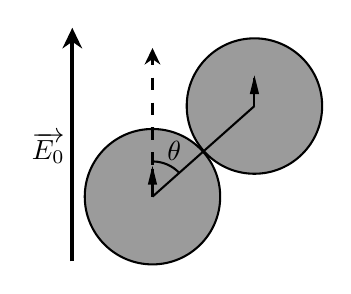
\begin{tikzpicture}[x=0.75pt,y=0.75pt,yscale=-0.75,xscale=0.75]
%uncomment if require: \path (0,465); %set diagram left start at 0, and has height of 465
%Shape: Circle [id:dp7322542907006744] 
\draw  [fill={rgb, 255:red, 155; green, 155; blue, 155 }  ,fill opacity=1 ] (332,316.5) .. controls (332,292.48) and (351.48,273) .. (375.5,273) .. controls (399.52,273) and (419,292.48) .. (419,316.5) .. controls (419,340.52) and (399.52,360) .. (375.5,360) .. controls (351.48,360) and (332,340.52) .. (332,316.5) -- cycle ;
%Straight Lines [id:da7555008022550928] 
\draw  [dash pattern={on 4.5pt off 4.5pt}]  (375.5,224) -- (375.5,316.5) ;
\draw [shift={(375.5,221)}, rotate = 90] [fill={rgb, 255:red, 0; green, 0; blue, 0 }  ][line width=0.08]  [draw opacity=0] (10.72,-5.15) -- (0,0) -- (10.72,5.15) -- (7.12,0) -- cycle    ;
%Shape: Arc [id:dp17914322281357842] 
\draw  [draw opacity=0] (376.12,293.87) .. controls (382.59,294.04) and (388.4,296.76) .. (392.52,301.03) -- (375.5,316.5) -- cycle ; \draw   (376.12,293.87) .. controls (382.59,294.04) and (388.4,296.76) .. (392.52,301.03) ;
%Straight Lines [id:da9918169411952207] 
\draw    (375.5,298.77) -- (375.5,316.5) ;
\draw [shift={(375.5,296.77)}, rotate = 90] [fill={rgb, 255:red, 0; green, 0; blue, 0 }  ][line width=0.08]  [draw opacity=0] (12,-3) -- (0,0) -- (12,3) -- cycle    ;
%Shape: Circle [id:dp25884969376134515] 
\draw  [fill={rgb, 255:red, 155; green, 155; blue, 155 }  ,fill opacity=1 ] (397.5,258.27) .. controls (397.5,234.25) and (416.98,214.77) .. (441,214.77) .. controls (465.02,214.77) and (484.5,234.25) .. (484.5,258.27) .. controls (484.5,282.3) and (465.02,301.77) .. (441,301.77) .. controls (416.98,301.77) and (397.5,282.3) .. (397.5,258.27) -- cycle ;
%Straight Lines [id:da8523540848862873] 
\draw    (441,240.55) -- (441,258.27) ;
\draw [shift={(441,238.55)}, rotate = 90] [fill={rgb, 255:red, 0; green, 0; blue, 0 }  ][line width=0.08]  [draw opacity=0] (12,-3) -- (0,0) -- (12,3) -- cycle    ;
%Straight Lines [id:da9816229971397216] 
\draw    (441,258.27) -- (375.5,316.5) ;
%Straight Lines [id:da11376192280629949] 
\draw [line width=1.5]    (324,358) -- (324,212) ;
\draw [shift={(324,208)}, rotate = 450] [fill={rgb, 255:red, 0; green, 0; blue, 0 }  ][line width=0.08]  [draw opacity=0] (13.4,-6.43) -- (0,0) -- (13.4,6.44) -- (8.9,0) -- cycle    ;

% Text Node
\draw (383,278.9) node [anchor=north west][inner sep=0.75pt]    {$\theta $};
% Text Node
\draw (296,273.4) node [anchor=north west][inner sep=0.75pt]  [color={rgb, 255:red, 0; green, 0; blue, 0 }  ,opacity=1 ]  {$\overrightarrow{E_{0}}$};
\end{tikzpicture}\\
Hình $1$.
        \end{center}
       \item Hãy tính các năng lượng tương tác lưỡng cực $-$ lưỡng cực cho ba cách sắp xếp cấu hình như trên các hình dưới đây:
       \begin{center}

\tikzset{every picture/.style={line width=0.75pt}} %set default line width to 0.75pt        

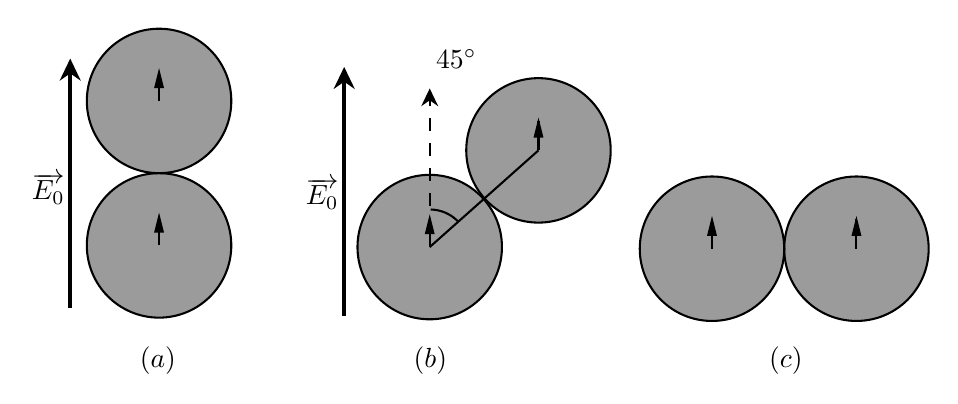
\begin{tikzpicture}[x=0.75pt,y=0.75pt,yscale=-0.8,xscale=0.8]
%uncomment if require: \path (0,465); %set diagram left start at 0, and has height of 465

%Shape: Circle [id:dp7992342857810553] 
\draw  [fill={rgb, 255:red, 155; green, 155; blue, 155 }  ,fill opacity=1 ] (503,324.5) .. controls (503,300.48) and (522.48,281) .. (546.5,281) .. controls (570.52,281) and (590,300.48) .. (590,324.5) .. controls (590,348.52) and (570.52,368) .. (546.5,368) .. controls (522.48,368) and (503,348.52) .. (503,324.5) -- cycle ;
%Shape: Circle [id:dp14786583206625825] 
\draw  [fill={rgb, 255:red, 155; green, 155; blue, 155 }  ,fill opacity=1 ] (416,324.5) .. controls (416,300.48) and (435.48,281) .. (459.5,281) .. controls (483.52,281) and (503,300.48) .. (503,324.5) .. controls (503,348.52) and (483.52,368) .. (459.5,368) .. controls (435.48,368) and (416,348.52) .. (416,324.5) -- cycle ;
%Shape: Circle [id:dp43921552368924277] 
\draw  [fill={rgb, 255:red, 155; green, 155; blue, 155 }  ,fill opacity=1 ] (311.5,265.27) .. controls (311.5,241.25) and (330.98,221.77) .. (355,221.77) .. controls (379.02,221.77) and (398.5,241.25) .. (398.5,265.27) .. controls (398.5,289.3) and (379.02,308.77) .. (355,308.77) .. controls (330.98,308.77) and (311.5,289.3) .. (311.5,265.27) -- cycle ;
%Shape: Circle [id:dp25575605897945874] 
\draw  [fill={rgb, 255:red, 155; green, 155; blue, 155 }  ,fill opacity=1 ] (246,323.5) .. controls (246,299.48) and (265.48,280) .. (289.5,280) .. controls (313.52,280) and (333,299.48) .. (333,323.5) .. controls (333,347.52) and (313.52,367) .. (289.5,367) .. controls (265.48,367) and (246,347.52) .. (246,323.5) -- cycle ;
%Shape: Circle [id:dp30931649025827546] 
\draw  [fill={rgb, 255:red, 155; green, 155; blue, 155 }  ,fill opacity=1 ] (83,322.5) .. controls (83,298.48) and (102.48,279) .. (126.5,279) .. controls (150.52,279) and (170,298.48) .. (170,322.5) .. controls (170,346.52) and (150.52,366) .. (126.5,366) .. controls (102.48,366) and (83,346.52) .. (83,322.5) -- cycle ;
%Shape: Circle [id:dp004553446595918276] 
\draw  [fill={rgb, 255:red, 155; green, 155; blue, 155 }  ,fill opacity=1 ] (83,235.5) .. controls (83,211.48) and (102.48,192) .. (126.5,192) .. controls (150.52,192) and (170,211.48) .. (170,235.5) .. controls (170,259.52) and (150.52,279) .. (126.5,279) .. controls (102.48,279) and (83,259.52) .. (83,235.5) -- cycle ;
%Straight Lines [id:da7555008022550928] 
\draw  [dash pattern={on 4.5pt off 4.5pt}]  (289.5,231) -- (289.5,323.5) ;
\draw [shift={(289.5,228)}, rotate = 90] [fill={rgb, 255:red, 0; green, 0; blue, 0 }  ][line width=0.08]  [draw opacity=0] (10.72,-5.15) -- (0,0) -- (10.72,5.15) -- (7.12,0) -- cycle    ;
%Shape: Arc [id:dp17914322281357842] 
\draw  [draw opacity=0] (290.12,300.87) .. controls (296.59,301.04) and (302.4,303.76) .. (306.52,308.03) -- (289.5,323.5) -- cycle ; \draw   (290.12,300.87) .. controls (296.59,301.04) and (302.4,303.76) .. (306.52,308.03) ;
%Straight Lines [id:da9918169411952207] 
\draw    (289.5,305.77) -- (289.5,323.5) ;
\draw [shift={(289.5,303.77)}, rotate = 90] [fill={rgb, 255:red, 0; green, 0; blue, 0 }  ][line width=0.08]  [draw opacity=0] (12,-3) -- (0,0) -- (12,3) -- cycle    ;
%Straight Lines [id:da8523540848862873] 
\draw    (355,247.55) -- (355,265.27) ;
\draw [shift={(355,245.55)}, rotate = 90] [fill={rgb, 255:red, 0; green, 0; blue, 0 }  ][line width=0.08]  [draw opacity=0] (12,-3) -- (0,0) -- (12,3) -- cycle    ;
%Straight Lines [id:da9816229971397216] 
\draw    (355,265.27) -- (289.5,323.5) ;
%Straight Lines [id:da11376192280629949] 
\draw [line width=1.5]    (238,365) -- (238,219) ;
\draw [shift={(238,215)}, rotate = 450] [fill={rgb, 255:red, 0; green, 0; blue, 0 }  ][line width=0.08]  [draw opacity=0] (13.4,-6.43) -- (0,0) -- (13.4,6.44) -- (8.9,0) -- cycle    ;
%Straight Lines [id:da5581657313853913] 
\draw    (459.5,306.77) -- (459.5,324.5) ;
\draw [shift={(459.5,304.77)}, rotate = 90] [fill={rgb, 255:red, 0; green, 0; blue, 0 }  ][line width=0.08]  [draw opacity=0] (12,-3) -- (0,0) -- (12,3) -- cycle    ;
%Straight Lines [id:da054358481868871156] 
\draw    (546.5,306.77) -- (546.5,324.5) ;
\draw [shift={(546.5,304.77)}, rotate = 90] [fill={rgb, 255:red, 0; green, 0; blue, 0 }  ][line width=0.08]  [draw opacity=0] (12,-3) -- (0,0) -- (12,3) -- cycle    ;
%Straight Lines [id:da610491834595927] 
\draw    (126.5,304.77) -- (126.5,322.5) ;
\draw [shift={(126.5,302.77)}, rotate = 90] [fill={rgb, 255:red, 0; green, 0; blue, 0 }  ][line width=0.08]  [draw opacity=0] (12,-3) -- (0,0) -- (12,3) -- cycle    ;
%Straight Lines [id:da2769093805455529] 
\draw    (126.5,217.77) -- (126.5,235.5) ;
\draw [shift={(126.5,215.77)}, rotate = 90] [fill={rgb, 255:red, 0; green, 0; blue, 0 }  ][line width=0.08]  [draw opacity=0] (12,-3) -- (0,0) -- (12,3) -- cycle    ;
%Straight Lines [id:da2395271006144144] 
\draw [line width=1.5]    (73,360) -- (73,214) ;
\draw [shift={(73,210)}, rotate = 450] [fill={rgb, 255:red, 0; green, 0; blue, 0 }  ][line width=0.08]  [draw opacity=0] (13.4,-6.43) -- (0,0) -- (13.4,6.44) -- (8.9,0) -- cycle    ;

% Text Node
\draw (213,280.4) node [anchor=north west][inner sep=0.75pt]  [color={rgb, 255:red, 0; green, 0; blue, 0 }  ,opacity=1 ]  {$\overrightarrow{E_{0}}$};
% Text Node
\draw (291.5,202.4) node [anchor=north west][inner sep=0.75pt]    {$45^\circ $};
% Text Node
\draw (48,277.4) node [anchor=north west][inner sep=0.75pt]  [color={rgb, 255:red, 0; green, 0; blue, 0 }  ,opacity=1 ]  {$\overrightarrow{E_{0}}$};
% Text Node
\draw (113,381.4) node [anchor=north west][inner sep=0.75pt]    {$( a)$};
% Text Node
\draw (278,381.4) node [anchor=north west][inner sep=0.75pt]    {$( b)$};
% Text Node
\draw (492,381.4) node [anchor=north west][inner sep=0.75pt]    {$( c)$};


\end{tikzpicture}\\Hình $2$.
       \end{center}
       \item Hãy xác định xem cấu hình nào của hệ là cấu hình ổn định nhất.\\
        \textbf{Chú ý:} Trong các phép tính, mỗi quả cầu điện môi bị phân cực có thể được coi như một lưỡng cực điện đặt ở tâm quả cầu và năng lượng tương tác lưỡng cực - lưỡng cực có thể được biểu thị theo $p$ và $a$.
    \end{enumerate}
    \item Trong trường hợp có ba quả cầu trong chất lỏng, dựa trên các giả thiết như đề bài,
    \begin{enumerate}[a)]
        \item Tính các năng lượng tương tác lưỡng cực $-$ lưỡng cực cho ba cấu hình vẽ trên.
        \item Xác định xem cấu hình nào là cấu hình ổn định nhất.
        \item Xác định xem cấu hình nào là cấu hình kém ổn định nhất.
    \end{enumerate}
    \textbf{Chú ý:} Trong các phép tính, mỗi quả cầu điện môi bị phân cực có thể được coi như một lưỡng cực điện đặt ở tâm quả cầu, và năng lượng tương tác lưỡng cực $-$ lưỡng cực có thể được biểu thị theo $p$ và $a$.
\end{enumerate}
 \begin{center}


\tikzset{every picture/.style={line width=0.75pt}} %set default line width to 0.75pt        

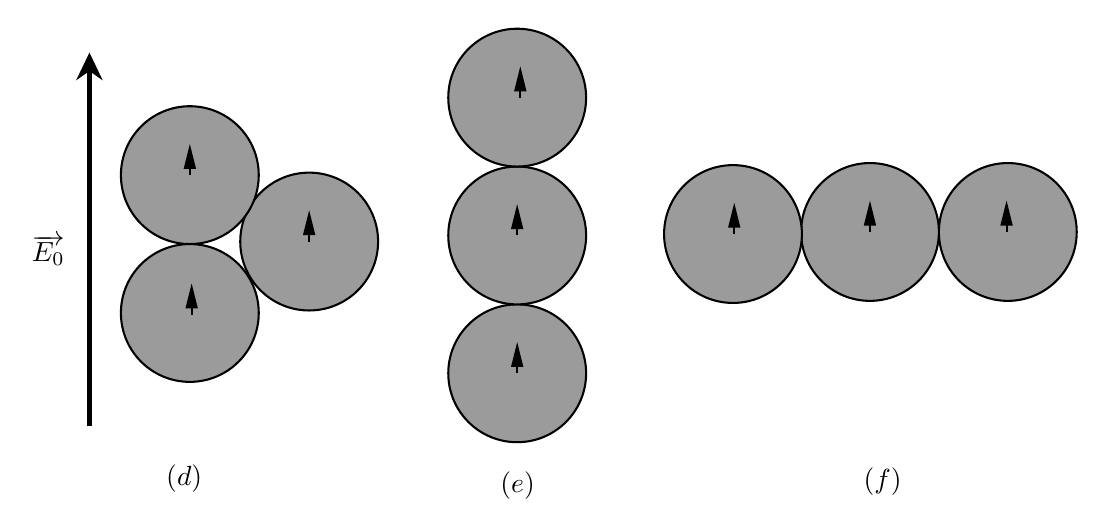
\begin{tikzpicture}[x=0.75pt,y=0.75pt,yscale=-1,xscale=1]
%uncomment if require: \path (0,465); %set diagram left start at 0, and has height of 465

%Shape: Circle [id:dp4339641994583381] 
\draw  [fill={rgb, 255:red, 155; green, 155; blue, 155 }  ,fill opacity=1 ] (480.76,268.51) .. controls (480.76,250.17) and (495.63,235.31) .. (513.97,235.31) .. controls (532.3,235.31) and (547.17,250.17) .. (547.17,268.51) .. controls (547.17,286.85) and (532.3,301.71) .. (513.97,301.71) .. controls (495.63,301.71) and (480.76,286.85) .. (480.76,268.51) -- cycle ;
%Shape: Circle [id:dp052224911367229065] 
\draw  [fill={rgb, 255:red, 155; green, 155; blue, 155 }  ,fill opacity=1 ] (414.36,268.51) .. controls (414.36,250.17) and (429.22,235.31) .. (447.56,235.31) .. controls (465.9,235.31) and (480.76,250.17) .. (480.76,268.51) .. controls (480.76,286.85) and (465.9,301.71) .. (447.56,301.71) .. controls (429.22,301.71) and (414.36,286.85) .. (414.36,268.51) -- cycle ;
%Shape: Circle [id:dp6035501274955883] 
\draw  [fill={rgb, 255:red, 155; green, 155; blue, 155 }  ,fill opacity=1 ] (348.36,269.51) .. controls (348.36,251.17) and (363.22,236.31) .. (381.56,236.31) .. controls (399.9,236.31) and (414.76,251.17) .. (414.76,269.51) .. controls (414.76,287.85) and (399.9,302.71) .. (381.56,302.71) .. controls (363.22,302.71) and (348.36,287.85) .. (348.36,269.51) -- cycle ;
%Shape: Circle [id:dp5029663370925965] 
\draw  [fill={rgb, 255:red, 155; green, 155; blue, 155 }  ,fill opacity=1 ] (244.38,336.61) .. controls (244.38,318.27) and (259.25,303.41) .. (277.58,303.41) .. controls (295.92,303.41) and (310.79,318.27) .. (310.79,336.61) .. controls (310.79,354.95) and (295.92,369.81) .. (277.58,369.81) .. controls (259.25,369.81) and (244.38,354.95) .. (244.38,336.61) -- cycle ;
%Shape: Circle [id:dp8698943026356059] 
\draw  [fill={rgb, 255:red, 155; green, 155; blue, 155 }  ,fill opacity=1 ] (244.38,270.2) .. controls (244.38,251.87) and (259.25,237) .. (277.58,237) .. controls (295.92,237) and (310.79,251.87) .. (310.79,270.2) .. controls (310.79,288.54) and (295.92,303.41) .. (277.58,303.41) .. controls (259.25,303.41) and (244.38,288.54) .. (244.38,270.2) -- cycle ;
%Shape: Circle [id:dp9184176268049609] 
\draw  [fill={rgb, 255:red, 155; green, 155; blue, 155 }  ,fill opacity=1 ] (244.38,203.8) .. controls (244.38,185.46) and (259.25,170.59) .. (277.58,170.59) .. controls (295.92,170.59) and (310.79,185.46) .. (310.79,203.8) .. controls (310.79,222.13) and (295.92,237) .. (277.58,237) .. controls (259.25,237) and (244.38,222.13) .. (244.38,203.8) -- cycle ;
%Shape: Circle [id:dp26146197647762914] 
\draw  [fill={rgb, 255:red, 155; green, 155; blue, 155 }  ,fill opacity=1 ] (144.16,273.14) .. controls (144.16,254.8) and (159.03,239.93) .. (177.36,239.93) .. controls (195.7,239.93) and (210.57,254.8) .. (210.57,273.14) .. controls (210.57,291.47) and (195.7,306.34) .. (177.36,306.34) .. controls (159.03,306.34) and (144.16,291.47) .. (144.16,273.14) -- cycle ;
%Shape: Circle [id:dp574949835208366] 
\draw  [fill={rgb, 255:red, 155; green, 155; blue, 155 }  ,fill opacity=1 ] (86.66,241.14) .. controls (86.66,222.8) and (101.53,207.93) .. (119.87,207.93) .. controls (138.2,207.93) and (153.07,222.8) .. (153.07,241.14) .. controls (153.07,259.47) and (138.2,274.34) .. (119.87,274.34) .. controls (101.53,274.34) and (86.66,259.47) .. (86.66,241.14) -- cycle ;
%Shape: Circle [id:dp5531728679179251] 
\draw  [fill={rgb, 255:red, 155; green, 155; blue, 155 }  ,fill opacity=1 ] (86.66,307.54) .. controls (86.66,289.2) and (101.53,274.34) .. (119.87,274.34) .. controls (138.2,274.34) and (153.07,289.2) .. (153.07,307.54) .. controls (153.07,325.88) and (138.2,340.74) .. (119.87,340.74) .. controls (101.53,340.74) and (86.66,325.88) .. (86.66,307.54) -- cycle ;
%Straight Lines [id:da660486440076847] 
\draw    (120.75,295.31) -- (120.75,308.37) ;
\draw [shift={(120.75,293.31)}, rotate = 90] [fill={rgb, 255:red, 0; green, 0; blue, 0 }  ][line width=0.08]  [draw opacity=0] (12,-3) -- (0,0) -- (12,3) -- cycle    ;
%Straight Lines [id:da17362894362800052] 
\draw    (382.16,256.45) -- (382.16,269.51) ;
\draw [shift={(382.16,254.45)}, rotate = 90] [fill={rgb, 255:red, 0; green, 0; blue, 0 }  ][line width=0.08]  [draw opacity=0] (12,-3) -- (0,0) -- (12,3) -- cycle    ;
%Straight Lines [id:da2495028442818401] 
\draw    (447.56,255.45) -- (447.56,268.51) ;
\draw [shift={(447.56,253.45)}, rotate = 90] [fill={rgb, 255:red, 0; green, 0; blue, 0 }  ][line width=0.08]  [draw opacity=0] (12,-3) -- (0,0) -- (12,3) -- cycle    ;
%Straight Lines [id:da7441244508416673] 
\draw    (277.58,323.55) -- (277.58,336.61) ;
\draw [shift={(277.58,321.55)}, rotate = 90] [fill={rgb, 255:red, 0; green, 0; blue, 0 }  ][line width=0.08]  [draw opacity=0] (12,-3) -- (0,0) -- (12,3) -- cycle    ;
%Straight Lines [id:da4570383736591437] 
\draw    (277.58,257.15) -- (277.58,270.2) ;
\draw [shift={(277.58,255.15)}, rotate = 90] [fill={rgb, 255:red, 0; green, 0; blue, 0 }  ][line width=0.08]  [draw opacity=0] (12,-3) -- (0,0) -- (12,3) -- cycle    ;
%Straight Lines [id:da4911642488394289] 
\draw [line width=1.5]    (71.49,362.23) -- (71.49,186.09) ;
\draw [shift={(71.49,182.09)}, rotate = 450] [fill={rgb, 255:red, 0; green, 0; blue, 0 }  ][line width=0.08]  [draw opacity=0] (13.4,-6.43) -- (0,0) -- (13.4,6.44) -- (8.9,0) -- cycle    ;
%Straight Lines [id:da7818527846742416] 
\draw    (513.36,255.45) -- (513.36,268.51) ;
\draw [shift={(513.36,253.45)}, rotate = 90] [fill={rgb, 255:red, 0; green, 0; blue, 0 }  ][line width=0.08]  [draw opacity=0] (12,-3) -- (0,0) -- (12,3) -- cycle    ;
%Straight Lines [id:da3914857405478256] 
\draw    (279.08,190.74) -- (279.08,203.8) ;
\draw [shift={(279.08,188.74)}, rotate = 90] [fill={rgb, 255:red, 0; green, 0; blue, 0 }  ][line width=0.08]  [draw opacity=0] (12,-3) -- (0,0) -- (12,3) -- cycle    ;
%Straight Lines [id:da18032882045365228] 
\draw    (119.87,228.08) -- (119.87,241.14) ;
\draw [shift={(119.87,226.08)}, rotate = 90] [fill={rgb, 255:red, 0; green, 0; blue, 0 }  ][line width=0.08]  [draw opacity=0] (12,-3) -- (0,0) -- (12,3) -- cycle    ;
%Straight Lines [id:da7341850230816754] 
\draw    (177.36,260.08) -- (177.36,273.14) ;
\draw [shift={(177.36,258.08)}, rotate = 90] [fill={rgb, 255:red, 0; green, 0; blue, 0 }  ][line width=0.08]  [draw opacity=0] (12,-3) -- (0,0) -- (12,3) -- cycle    ;

% Text Node
\draw (42.24,268.44) node [anchor=north west][inner sep=0.75pt]  [color={rgb, 255:red, 0; green, 0; blue, 0 }  ,opacity=1 ]  {$\overrightarrow{E_{0}}$};
% Text Node
\draw (107,379.4) node [anchor=north west][inner sep=0.75pt]    {$( d)$};
% Text Node
\draw (268,382.4) node [anchor=north west][inner sep=0.75pt]    {$( e)$};
% Text Node
\draw (443,380.4) node [anchor=north west][inner sep=0.75pt]    {$( f)$};


\end{tikzpicture}
 \end{center}
\end{vd}
\begin{loigiai}
\begin{enumerate}[1)]                           
    \item Viết biểu thức năng lượng của tương tác lưỡng cực $-$ lưỡng cực giữa hai quả cầu điện môi nhỏ tiếp xúc với nhau theo $p$, $a$, và $\theta$.
    \begin{enumerate}[a)]
   \item Nếu đưa vào tọa độ cực, thành phần $z$ của điện trường sinh ra bởi một lưỡng cực đặt tại gốc với trục của nó song song với trục $z$ là:
    \[E_{z}(\theta, \phi)=-\dfrac{p}{4 \pi \varepsilon_{0}} \dfrac{1-3 \cos ^{2} \theta}{r^{3}}, \tag{1} \]
    trong đó $r$ là chiều dài của vector đơn vị tương đối của hai lưỡng cực. Trong điện trường ngoài $\ot E$, năng lượng của một lưỡng cực với trục của nó song song với trục $z$ là:
    \[U= -\ot{p}\cdot \ot{E}=-pE_{z}. \tag{2}\]
    Do đó, ta thu được kết quả năng lượng tương tác giữa hai quả cầu điện môi nhỏ tiếp xúc
    \[U_{12}=\dfrac{p^{2}}{4 \pi \varepsilon_{0}} \dfrac{1-3 \cos ^{2} \theta}{(2 a)^{3}}. \tag{3} \label{3d}\] 
    \item Tính các năng lượng tương tác lưỡng cực - lưỡng cực cho ba cấu hình trên:
    Trên cơ sở phương trình (\ref{3d}),
    \begin{itemize}
        \item Đối với cấu hình ($a$):
    \[U_{a}=\dfrac{1}{4 \pi \varepsilon_{0}} \dfrac{1-3}{(2 a)^{3}} p^{2}=-\dfrac{1}{4 \pi \varepsilon_{0}} \dfrac{p^{2}}{4 a^{3}}. \tag{4} \label{4d}\]
        \item  Đối với cấu hình ($b$): 
    \[U_{b}=\dfrac{1}{4 \pi \varepsilon_{0}} \dfrac{1-3 \cos ^{2} \dfrac{\pi}{4}}{(2 a)^{3}}=-\dfrac{1}{4 \pi \varepsilon_{0}} \dfrac{p^{2}}{16 a^{3}}. \tag{5} \label{5d} \]
        \item Đối với cấu hình ($c$):
    \[U_{c}=\dfrac{1}{4 \pi \varepsilon_{0}} \dfrac{1-0}{(2 a)^{3}} p^{2}=\dfrac{1}{4 \pi \varepsilon_{0}} \dfrac{p^{2}}{8 a^{3}}. \tag{6} \label{6d}\]
    \end{itemize}
    \item Việc so sánh (\ref{4d}), (\ref{5d}) và (\ref{6d}) chỉ ra rằng cấu hình ($a$) có năng lượng thấp nhất và nó tương ứng với trạng thái cơ bản của hệ. Đó là cấu hình ổn định nhất của hệ (theo nguyên lý thế năng cực tiểu).
    \end{enumerate}
    \item Ba quả cầu ($d$), ($e$) và ($f$).
   \begin{enumerate}[a)]
     \item Cách làm tương tự như ở phần trên.
     \begin{itemize}
         \item Đối với cấu hình ($d$), ta có:
     \[{U}_{{d}}=\dfrac{1}{4 \pi \varepsilon_{0}}\left(-\dfrac{{p}^{2}}{4 {a}^{3}}+2 \cdot \dfrac{{p}^{2}}{32 {a}^{3}}\right)=-\dfrac{1}{4 \pi \varepsilon_{0}} \dfrac{3 {p}^{2}}{16 {a}^{3}}. \tag{7}\]
     \item  Đối với cấu hình ($e$):
    \[{U}_{{e}}=\dfrac{1}{4 \pi \varepsilon_{0}}\left(-\dfrac{{p}^{2}}{4 {a}^{3}} \cdot 2-\dfrac{{p}^{2}}{32 {a}^{3}}\right)=-\dfrac{1}{4 \pi \varepsilon_{0}} \dfrac{17 {p}^{2}}{32 {a}^{3}}. \tag{8}\]
    \item Đối với cấu hình ($f$):
    \[{U}_{{f}}=\dfrac{1}{4 \pi \varepsilon_{0}}\left(\dfrac{{p}^{2}}{8 {a}^{3}} \cdot 2+\dfrac{{p}^{2}}{64 {a}^{3}}\right)=\dfrac{1}{4 \pi \varepsilon_{0}} \dfrac{17 {p}^{2}}{64 {a}^{3}}. \tag{9}\]
     \end{itemize}
  \item Cấu hình ($e$) có năng lượng thấp nhất và do đó nó ổn định nhất.
  \item Cấu hình ($f$) có năng lượng cao nhất và do đó kém ổn định nhất.
 \end{enumerate}
\end{enumerate}
\end{loigiai}


\begin{vd}[Bàn cờ dẫn điện]
Một bàn cờ $8\times 8$ cấu tạo từ các ô được làm từ hai loại kim loại, cả hai đều dẫn điện không tốt. Trong hệ còn hai phần tử khác đó là hai dải kim loại dẫn điện rất tốt chạy dọc hai viền của bàn cờ (dải tiếp xúc với dây nối như hình vẽ). Độ dày chung của bàn cờ và các ô là $t$ rất nhỏ hơn so với chiều dài $L$ của bàn cờ.
\begin{center}
    

\tikzset{every picture/.style={line width=0.75pt}} %set default line width to 0.75pt        

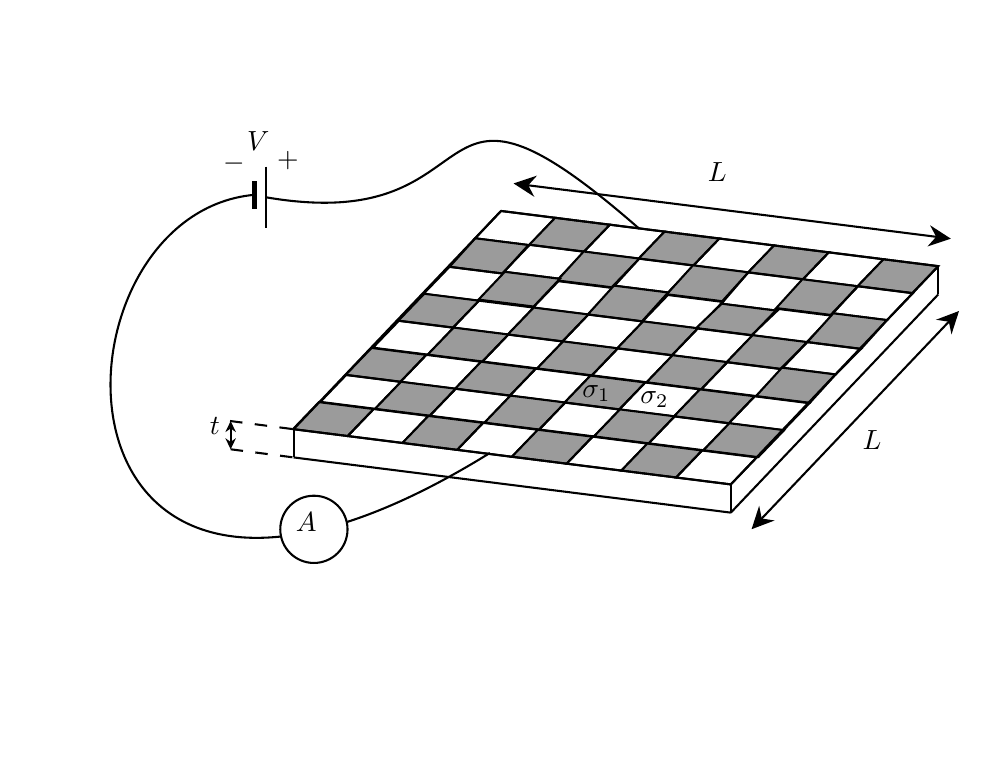
\begin{tikzpicture}[x=0.75pt,y=0.75pt,yscale=-1,xscale=1]
%uncomment if require: \path (0,470); %set diagram left start at 0, and has height of 470

%Shape: Parallelogram [id:dp1634681887307805] 
\draw   (282.36,141.41) -- (308.45,144.7) -- (296.01,157.87) -- (269.93,154.58) -- cycle ;
%Straight Lines [id:da7905958403536684] 
\draw    (182.41,246.55) -- (182.41,260.15) ;
%Shape: Parallelogram [id:dp9095361285915102] 
\draw  [fill={rgb, 255:red, 155; green, 155; blue, 155 }  ,fill opacity=1 ] (308.45,144.7) -- (334.81,148.03) -- (322.3,161.04) -- (295.93,157.71) -- cycle ;
%Shape: Parallelogram [id:dp7721525314718289] 
\draw   (334.81,148.03) -- (361.18,151.36) -- (348.67,164.37) -- (322.3,161.04) -- cycle ;
%Shape: Parallelogram [id:dp8016974778157118] 
\draw  [fill={rgb, 255:red, 155; green, 155; blue, 155 }  ,fill opacity=1 ] (361.18,151.36) -- (387.55,154.69) -- (375.04,167.7) -- (348.67,164.37) -- cycle ;
%Shape: Parallelogram [id:dp8022334304567804] 
\draw   (387.55,154.69) -- (413.92,158.02) -- (401.41,171.03) -- (375.04,167.69) -- cycle ;
%Shape: Parallelogram [id:dp07696832150226673] 
\draw  [fill={rgb, 255:red, 155; green, 155; blue, 155 }  ,fill opacity=1 ] (413.92,158.01) -- (440.29,161.34) -- (427.78,174.35) -- (401.41,171.02) -- cycle ;
%Shape: Parallelogram [id:dp9645533748108515] 
\draw   (440.29,161.34) -- (466.66,164.67) -- (454.14,177.68) -- (427.78,174.35) -- cycle ;
%Shape: Parallelogram [id:dp6649476659417421] 
\draw  [fill={rgb, 255:red, 155; green, 155; blue, 155 }  ,fill opacity=1 ] (466.66,164.67) -- (493.03,168) -- (480.51,181.01) -- (454.14,177.68) -- cycle ;
%Shape: Parallelogram [id:dp677898638583595] 
\draw  [fill={rgb, 255:red, 155; green, 155; blue, 155 }  ,fill opacity=1 ] (269.93,154.58) -- (295.54,157.81) -- (283.16,171.55) -- (257.56,168.32) -- cycle ;
%Shape: Parallelogram [id:dp10735060125369023] 
\draw   (296.26,157.68) -- (322.63,161.01) -- (310.11,174.02) -- (283.74,170.69) -- cycle ;
%Shape: Parallelogram [id:dp9088792048232939] 
\draw  [fill={rgb, 255:red, 155; green, 155; blue, 155 }  ,fill opacity=1 ] (322.17,160.95) -- (348.99,164.34) -- (336.07,178.52) -- (309.25,175.14) -- cycle ;
%Shape: Parallelogram [id:dp4500605468061303] 
\draw   (348.99,164.34) -- (375.36,167.67) -- (362.85,180.68) -- (336.48,177.34) -- cycle ;
%Shape: Parallelogram [id:dp7488763500831803] 
\draw  [fill={rgb, 255:red, 155; green, 155; blue, 155 }  ,fill opacity=1 ] (374.85,167.6) -- (401.54,170.97) -- (388.67,185.16) -- (361.99,181.79) -- cycle ;
%Shape: Parallelogram [id:dp4846791851214096] 
\draw   (401.54,170.97) -- (428.1,174.32) -- (415.1,189.43) -- (388.53,186.08) -- cycle ;
%Shape: Parallelogram [id:dp8925225920275939] 
\draw  [fill={rgb, 255:red, 155; green, 155; blue, 155 }  ,fill opacity=1 ] (427.55,174.32) -- (454.14,177.68) -- (441.32,191.81) -- (414.72,188.45) -- cycle ;
%Shape: Parallelogram [id:dp7035911290176065] 
\draw   (454.47,177.65) -- (480.84,180.98) -- (468.33,193.99) -- (441.96,190.66) -- cycle ;
%Shape: Parallelogram [id:dp11292783009809115] 
\draw   (257.56,168.32) -- (283.92,171.65) -- (271.41,184.66) -- (245.04,181.33) -- cycle ;
%Shape: Parallelogram [id:dp8268722870196277] 
\draw  [fill={rgb, 255:red, 155; green, 155; blue, 155 }  ,fill opacity=1 ] (284.17,170.74) -- (310.71,174.09) -- (298.06,187.46) -- (271.52,184.11) -- cycle ;
%Shape: Parallelogram [id:dp04735681570813077] 
\draw   (310.29,174.98) -- (336.66,178.31) -- (324.15,191.32) -- (297.78,187.98) -- cycle ;
%Shape: Parallelogram [id:dp9134129539151328] 
\draw  [fill={rgb, 255:red, 155; green, 155; blue, 155 }  ,fill opacity=1 ] (336.75,177.38) -- (362.85,180.68) -- (350.25,194.61) -- (324.15,191.31) -- cycle ;
%Shape: Parallelogram [id:dp42332262246839125] 
\draw   (363.03,181.63) -- (389.4,184.96) -- (376.89,197.97) -- (350.52,194.64) -- cycle ;
%Shape: Parallelogram [id:dp9586661387599467] 
\draw  [fill={rgb, 255:red, 155; green, 155; blue, 155 }  ,fill opacity=1 ] (388.69,186.1) -- (415.48,189.48) -- (403.04,201.33) -- (376.25,197.95) -- cycle ;
%Shape: Parallelogram [id:dp3897134042089663] 
\draw   (415.77,188.29) -- (442.14,191.62) -- (429.62,204.63) -- (403.25,201.3) -- cycle ;
%Shape: Parallelogram [id:dp23824795071231386] 
\draw  [fill={rgb, 255:red, 155; green, 155; blue, 155 }  ,fill opacity=1 ] (442.45,190.72) -- (468.33,193.99) -- (455.82,207.86) -- (429.95,204.59) -- cycle ;
%Shape: Parallelogram [id:dp3136329722838067] 
\draw  [fill={rgb, 255:red, 155; green, 155; blue, 155 }  ,fill opacity=1 ] (245.37,181.3) -- (271.74,184.63) -- (259.22,197.64) -- (232.85,194.31) -- cycle ;
%Shape: Parallelogram [id:dp30533494177104537] 
\draw   (271.74,184.63) -- (298.1,187.96) -- (285.59,200.97) -- (259.22,197.63) -- cycle ;
%Shape: Parallelogram [id:dp4712679864699516] 
\draw  [fill={rgb, 255:red, 155; green, 155; blue, 155 }  ,fill opacity=1 ] (298.1,187.95) -- (324.47,191.28) -- (311.96,204.29) -- (285.59,200.96) -- cycle ;
%Shape: Parallelogram [id:dp7986379838493471] 
\draw   (324.47,191.28) -- (350.84,194.61) -- (338.33,207.62) -- (311.96,204.29) -- cycle ;
%Shape: Parallelogram [id:dp32661269944620597] 
\draw  [fill={rgb, 255:red, 155; green, 155; blue, 155 }  ,fill opacity=1 ] (350.84,194.61) -- (377.21,197.94) -- (364.7,210.95) -- (338.33,207.62) -- cycle ;
%Shape: Parallelogram [id:dp03575534689371507] 
\draw   (377.21,197.94) -- (403.58,201.27) -- (391.07,214.28) -- (364.7,210.95) -- cycle ;
%Shape: Parallelogram [id:dp0424514191210299] 
\draw  [fill={rgb, 255:red, 155; green, 155; blue, 155 }  ,fill opacity=1 ] (403.58,201.27) -- (429.95,204.6) -- (417.44,217.61) -- (391.07,214.28) -- cycle ;
%Shape: Parallelogram [id:dp1742319089301827] 
\draw   (429.82,204.58) -- (455.82,207.86) -- (443.58,220.18) -- (417.58,216.9) -- cycle ;
%Shape: Parallelogram [id:dp8218078558084174] 
\draw   (233.18,194.28) -- (259.55,197.61) -- (247.03,210.62) -- (220.66,207.28) -- cycle ;
%Shape: Parallelogram [id:dp5436912131639109] 
\draw  [fill={rgb, 255:red, 155; green, 155; blue, 155 }  ,fill opacity=1 ] (259.55,197.6) -- (285.92,200.93) -- (273.4,213.94) -- (247.03,210.61) -- cycle ;
%Shape: Parallelogram [id:dp7999141912617251] 
\draw   (285.92,200.93) -- (312.28,204.26) -- (299.77,217.27) -- (273.4,213.94) -- cycle ;
%Shape: Parallelogram [id:dp24240463688042935] 
\draw  [fill={rgb, 255:red, 155; green, 155; blue, 155 }  ,fill opacity=1 ] (312.28,204.26) -- (338.65,207.59) -- (326.14,220.6) -- (299.77,217.27) -- cycle ;
%Shape: Parallelogram [id:dp33547683393523164] 
\draw   (338.65,207.59) -- (365.02,210.92) -- (352.51,223.93) -- (326.14,220.6) -- cycle ;
%Shape: Parallelogram [id:dp8314802344905496] 
\draw  [fill={rgb, 255:red, 155; green, 155; blue, 155 }  ,fill opacity=1 ] (365.02,210.92) -- (391.39,214.25) -- (378.88,227.26) -- (352.51,223.93) -- cycle ;
%Shape: Parallelogram [id:dp5766289321028972] 
\draw   (391.39,214.25) -- (417.76,217.58) -- (405.25,230.58) -- (378.88,227.25) -- cycle ;
%Shape: Parallelogram [id:dp24314540320655564] 
\draw  [fill={rgb, 255:red, 155; green, 155; blue, 155 }  ,fill opacity=1 ] (417.71,216.91) -- (443.58,220.18) -- (431.12,233.85) -- (405.25,230.58) -- cycle ;
%Shape: Parallelogram [id:dp8343652516667763] 
\draw  [fill={rgb, 255:red, 155; green, 155; blue, 155 }  ,fill opacity=1 ] (220,207.4) -- (246.37,210.74) -- (233.86,223.74) -- (207.49,220.41) -- cycle ;
%Shape: Parallelogram [id:dp002049087379289549] 
\draw   (246.37,210.73) -- (272.74,214.06) -- (260.23,227.07) -- (233.86,223.74) -- cycle ;
%Shape: Parallelogram [id:dp6508141101896114] 
\draw  [fill={rgb, 255:red, 155; green, 155; blue, 155 }  ,fill opacity=1 ] (272.74,214.06) -- (299.11,217.39) -- (286.59,230.4) -- (260.23,227.07) -- cycle ;
%Shape: Parallelogram [id:dp9398739740832878] 
\draw   (299.11,217.39) -- (325.48,220.72) -- (312.96,233.73) -- (286.59,230.4) -- cycle ;
%Shape: Parallelogram [id:dp878136362323773] 
\draw  [fill={rgb, 255:red, 155; green, 155; blue, 155 }  ,fill opacity=1 ] (325.48,220.72) -- (351.84,224.05) -- (339.33,237.06) -- (312.96,233.73) -- cycle ;
%Shape: Parallelogram [id:dp48585372241904445] 
\draw   (351.84,224.05) -- (378.21,227.38) -- (365.7,240.39) -- (339.33,237.05) -- cycle ;
%Shape: Parallelogram [id:dp9069636410639039] 
\draw  [fill={rgb, 255:red, 155; green, 155; blue, 155 }  ,fill opacity=1 ] (378.21,227.37) -- (404.58,230.7) -- (392.07,243.71) -- (365.7,240.38) -- cycle ;
%Shape: Parallelogram [id:dp28895018888355795] 
\draw   (404.58,230.7) -- (430.95,234.03) -- (418.44,247.04) -- (392.07,243.71) -- cycle ;
%Shape: Parallelogram [id:dp43438181974774315] 
\draw   (207.81,220.38) -- (234.18,223.71) -- (221.67,236.72) -- (195.3,233.39) -- cycle ;
%Shape: Parallelogram [id:dp12315943525110495] 
\draw  [fill={rgb, 255:red, 155; green, 155; blue, 155 }  ,fill opacity=1 ] (234.18,223.71) -- (260.55,227.04) -- (248.04,240.05) -- (221.67,236.72) -- cycle ;
%Shape: Parallelogram [id:dp47358096089811585] 
\draw   (260.55,227.04) -- (286.92,230.37) -- (274.41,243.38) -- (248.04,240.05) -- cycle ;
%Shape: Parallelogram [id:dp34074785630316207] 
\draw  [fill={rgb, 255:red, 155; green, 155; blue, 155 }  ,fill opacity=1 ] (286.92,230.37) -- (313.29,233.7) -- (300.77,246.71) -- (274.41,243.38) -- cycle ;
%Shape: Parallelogram [id:dp1733943235092239] 
\draw   (313.29,233.7) -- (339.66,237.03) -- (327.14,250.04) -- (300.77,246.7) -- cycle ;
%Shape: Parallelogram [id:dp7440793240149637] 
\draw  [fill={rgb, 255:red, 155; green, 155; blue, 155 }  ,fill opacity=1 ] (339.66,237.02) -- (366.03,240.35) -- (353.51,253.36) -- (327.14,250.03) -- cycle ;
%Shape: Parallelogram [id:dp28203581002048206] 
\draw   (366.02,240.35) -- (392.39,243.68) -- (379.88,256.69) -- (353.51,253.36) -- cycle ;
%Shape: Parallelogram [id:dp17429886517884596] 
\draw  [fill={rgb, 255:red, 155; green, 155; blue, 155 }  ,fill opacity=1 ] (392.39,243.68) -- (418.76,247.01) -- (406.25,260.02) -- (379.88,256.69) -- cycle ;
%Shape: Parallelogram [id:dp5053273318057276] 
\draw  [fill={rgb, 255:red, 155; green, 155; blue, 155 }  ,fill opacity=1 ] (194.63,233.51) -- (221,236.84) -- (208.49,249.85) -- (182.12,246.52) -- cycle ;
%Shape: Parallelogram [id:dp5083307250794808] 
\draw   (221,236.84) -- (247.37,240.17) -- (234.86,253.18) -- (208.49,249.85) -- cycle ;
%Shape: Parallelogram [id:dp5030559914677115] 
\draw  [fill={rgb, 255:red, 155; green, 155; blue, 155 }  ,fill opacity=1 ] (247.37,240.17) -- (273.74,243.5) -- (261.23,256.51) -- (234.86,253.18) -- cycle ;
%Shape: Parallelogram [id:dp04149544633175206] 
\draw   (273.74,243.5) -- (300.11,246.83) -- (287.6,259.84) -- (261.23,256.5) -- cycle ;
%Shape: Parallelogram [id:dp9374124285190173] 
\draw  [fill={rgb, 255:red, 155; green, 155; blue, 155 }  ,fill opacity=1 ] (300.11,246.82) -- (326.48,250.16) -- (313.97,263.16) -- (287.6,259.83) -- cycle ;
%Shape: Parallelogram [id:dp7855595557469714] 
\draw   (326.48,250.15) -- (352.85,253.48) -- (340.33,266.49) -- (313.97,263.16) -- cycle ;
%Shape: Parallelogram [id:dp4211898209526288] 
\draw  [fill={rgb, 255:red, 155; green, 155; blue, 155 }  ,fill opacity=1 ] (352.85,253.48) -- (379.22,256.81) -- (366.7,269.82) -- (340.33,266.49) -- cycle ;
%Shape: Parallelogram [id:dp7899113190333609] 
\draw   (379.22,256.81) -- (405.59,260.14) -- (393.07,273.15) -- (366.7,269.82) -- cycle ;
%Straight Lines [id:da5873316786013936] 
\draw    (493.03,168) -- (493.03,181.6) ;
%Straight Lines [id:da5281811781936845] 
\draw    (493.03,168) -- (393.07,273.15) ;
%Straight Lines [id:da5356597417508657] 
\draw    (282.36,141.41) -- (182.41,246.55) ;
%Straight Lines [id:da45773821846578744] 
\draw    (493.03,181.6) -- (393.07,286.75) ;
%Straight Lines [id:da34297068964628274] 
\draw    (282.36,141.41) -- (493.03,168) ;
%Straight Lines [id:da8376418298814283] 
\draw    (182.41,246.55) -- (393.07,273.15) ;
%Straight Lines [id:da18951972627702118] 
\draw    (182.41,260.15) -- (393.07,286.75) ;
%Straight Lines [id:da5805655058728623] 
\draw    (393.07,273.15) -- (393.07,286.75) ;
%Straight Lines [id:da6481821546126103] 
\draw    (291.39,128.53) -- (496.1,154.37) ;
\draw [shift={(499.07,154.75)}, rotate = 187.2] [fill={rgb, 255:red, 0; green, 0; blue, 0 }  ][line width=0.08]  [draw opacity=0] (10.72,-5.15) -- (0,0) -- (10.72,5.15) -- (7.12,0) -- cycle    ;
\draw [shift={(288.41,128.15)}, rotate = 7.2] [fill={rgb, 255:red, 0; green, 0; blue, 0 }  ][line width=0.08]  [draw opacity=0] (10.72,-5.15) -- (0,0) -- (10.72,5.15) -- (7.12,0) -- cycle    ;
%Straight Lines [id:da8210838899287984] 
\draw    (500.96,191.77) -- (405.14,292.57) ;
\draw [shift={(403.07,294.75)}, rotate = 313.55] [fill={rgb, 255:red, 0; green, 0; blue, 0 }  ][line width=0.08]  [draw opacity=0] (10.72,-5.15) -- (0,0) -- (10.72,5.15) -- (7.12,0) -- cycle    ;
\draw [shift={(503.03,189.6)}, rotate = 133.55] [fill={rgb, 255:red, 0; green, 0; blue, 0 }  ][line width=0.08]  [draw opacity=0] (10.72,-5.15) -- (0,0) -- (10.72,5.15) -- (7.12,0) -- cycle    ;
%Straight Lines [id:da28792563006672633] 
\draw  [dash pattern={on 4.5pt off 4.5pt}]  (151.8,242.6) -- (182.12,246.52) ;
%Straight Lines [id:da8630355929059936] 
\draw  [dash pattern={on 4.5pt off 4.5pt}]  (152.09,256.23) -- (182.41,260.15) ;
%Straight Lines [id:da502164850868569] 
\draw    (152.09,245.63) -- (152.09,253.23) ;
\draw [shift={(152.09,256.23)}, rotate = 270] [fill={rgb, 255:red, 0; green, 0; blue, 0 }  ][line width=0.08]  [draw opacity=0] (5.36,-2.57) -- (0,0) -- (5.36,2.57) -- (3.56,0) -- cycle    ;
\draw [shift={(152.09,242.63)}, rotate = 90] [fill={rgb, 255:red, 0; green, 0; blue, 0 }  ][line width=0.08]  [draw opacity=0] (5.36,-2.57) -- (0,0) -- (5.36,2.57) -- (3.56,0) -- cycle    ;
%Straight Lines [id:da8697444809472166] 
\draw [line width=1.5]    (163.55,127.04) -- (163.55,140.6) ;
%Straight Lines [id:da021032614299149932] 
\draw    (169,120) -- (169,149.6) ;
%Curve Lines [id:da1748810964647569] 
\draw    (163.8,133.6) .. controls (58.8,142.6) and (54.8,395.6) .. (277,258) ;
%Curve Lines [id:da4611407963859848] 
\draw    (169,134.8) .. controls (283.8,154.6) and (238.8,53.6) .. (349,150) ;
%Flowchart: Connector [id:dp2209190587861436] 
\draw  [fill={rgb, 255:red, 255; green, 255; blue, 255 }  ,fill opacity=1 ] (176,294.8) .. controls (176,285.85) and (183.25,278.6) .. (192.2,278.6) .. controls (201.15,278.6) and (208.4,285.85) .. (208.4,294.8) .. controls (208.4,303.75) and (201.15,311) .. (192.2,311) .. controls (183.25,311) and (176,303.75) .. (176,294.8) -- cycle ;


% Text Node
\draw (147,112.4) node [anchor=north west][inner sep=0.75pt]    {$-$};
% Text Node
\draw (173,111.4) node [anchor=north west][inner sep=0.75pt]    {$+$};
% Text Node
\draw (158.55,101.44) node [anchor=north west][inner sep=0.75pt]    {$V$};
% Text Node
\draw (182,285.4) node [anchor=north west][inner sep=0.75pt]    {$A$};
% Text Node
\draw (320,224) node [anchor=north west][inner sep=0.75pt]    {$\sigma _{1}$};
% Text Node
\draw (348,227) node [anchor=north west][inner sep=0.75pt]    {$\sigma _{2}$};
% Text Node
\draw (380.55,116.44) node [anchor=north west][inner sep=0.75pt]    {$L$};
% Text Node
\draw (455.05,245.57) node [anchor=north west][inner sep=0.75pt]    {$L$};
% Text Node
\draw (140.55,239.44) node [anchor=north west][inner sep=0.75pt]    {$t$};
\end{tikzpicture}
\end{center}
Độ dẫn điện của ô màu trắng là $\sigma_1$, của ô màu tối là $\sigma_2$. Tìm dòng điện chạy qua bàn cờ nếu một hiệu điện thế $V$ được đặt vào hai điện cực, bỏ qua điện trở của các điểm tiếp xúc.
\end{vd}

\begin{loigiai}
Nếu tất cả các ô trên bàn cờ đều làm từ một kim loại đồng nhất có độ dẫn điện $\sigma_1$, thì độ lớn điện trường trong bàn cờ sẽ là $E=\dfrac{V}{L}$ và mật độ dòng điện là 
$$j_1=\sigma_1.E,$$ và cường độ dòng điện chạy trong bản sẽ là
$$I_1=j_1Lt=\sigma_1ELt=V\sigma_1t.$$
Tương tự nếu cả bàn cờ làm bằng kim loại đồng nhất có độ dẫn điện $\sigma_2$, với cùng một điện thế $V$, dòng $I_2$ chạy qua bàn cờ sẽ là $V.\sigma_2.t$. Lưu ý rằng cường độ dòng điện chạy trong bàn cờ không phụ thuộc vào độ dài $L$ của bản.
\\Theo hướng suy luận như thế, chúng ta dự đoán cường độ dòng chạy qua bàn cờ thật sẽ là trung bình nhân của hai dòng điện trên, và chúng ta phải đi chứng minh điều này là đúng 
$$I=Vt\sqrt{\sigma_1 \sigma_2}.$$
 Suy luận này là đúng đối với mọi bàn cờ đan xen có độ dày đồng nhất nếu chúng thỏa mãn các điều kiện sau
   \\ Nếu tồn tại hai điểm $A$ và $B$ sao cho chúng có thể thay thế vị trí của nhau trên bàn cờ bằng cách quay bàn cờ $90^\circ$, thì  tích độ dẫn điện của hai điểm đó phải có giá trị độc lập dù cho ta chọn hai điểm đó bằng bất kì cách nào
    \\ Đối với bài toán điều kiện này đương nhiên thỏa mãn vì nếu ta xoay bàn cờ $90^\circ$ thì ô đen luôn bị đổi chỗ bởi các ô trắng và ngược lại, do đó điểm $A$ và $B$ luôn có màu khác nhau nên tích độ dẫn điện $\sigma_A.\sigma_B$ luôn bằng $\sigma_1.\sigma_2$ không đổi.
    \\ Tiếp theo để đơn giản hóa bài toán, thay vì dùng bàn cờ thông thường ta sẽ chỉ xét một mạng 2x2 ô cờ vì chúng cũng thỏa mãn đầy đủ tính chất nêu trên. Đầu tiên chúng ta nghiên cứu về điện trường trong mạng và sau đó là dòng điện chạy qua từng ô vuông của mạng. Điện trường nội tại có thể được xác định hoàn toàn bằng điện thế, được kí hiệu là ($\phi$) và được minh họa trực quan bằng các đường đẳng thế, biểu diễn bằng các đường cắt chéo như hình 1.
    \begin{center}
        

\tikzset{every picture/.style={line width=0.75pt}} %set default line width to 0.75pt        

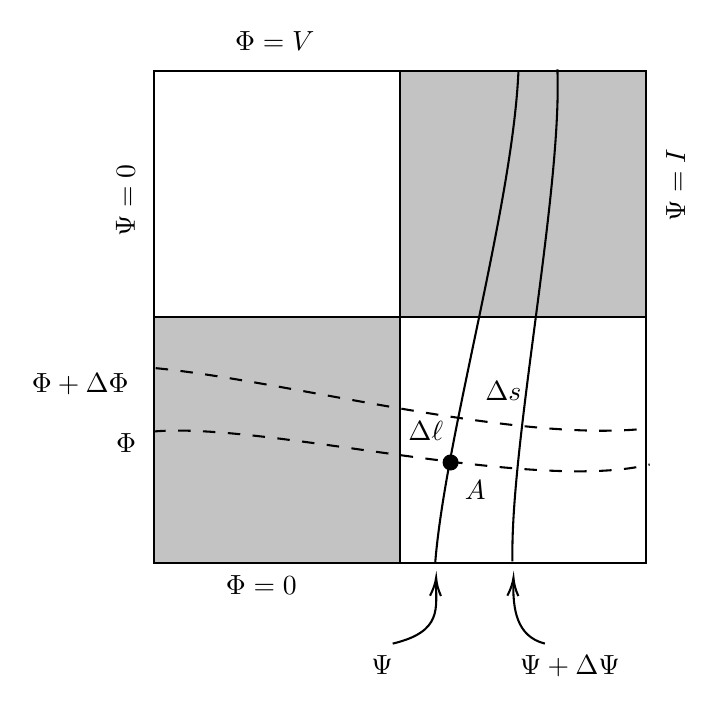
\begin{tikzpicture}[x=0.75pt,y=0.75pt,yscale=-0.8,xscale=0.8]
%uncomment if require: \path (0,493); %set diagram left start at 0, and has height of 493

%Shape: Square [id:dp35765568233416056] 
\draw   (173.81,63.44) -- (321.96,63.44) -- (321.96,211.59) -- (173.81,211.59) -- cycle ;
%Shape: Square [id:dp44032875059918886] 
\draw  [fill={rgb, 255:red, 155; green, 155; blue, 155 }  ,fill opacity=0.6 ] (321.96,63.44) -- (470.11,63.44) -- (470.11,211.59) -- (321.96,211.59) -- cycle ;
%Shape: Rectangle [id:dp3323113313608652] 
\draw  [fill={rgb, 255:red, 155; green, 155; blue, 155 }  ,fill opacity=0.6 ] (173.81,211.59) -- (321.96,211.59) -- (321.96,359.74) -- (173.81,359.74) -- cycle ;
%Shape: Rectangle [id:dp7482873919160049] 
\draw   (321.96,211.59) -- (470.11,211.59) -- (470.11,359.74) -- (321.96,359.74) -- cycle ;
%Curve Lines [id:da7792535041822144] 
\draw    (343,360.04) .. controls (349.01,283.71) and (389.57,145.48) .. (393.18,63.44) ;
%Curve Lines [id:da20272580305573973] 
\draw    (389.57,358.54) .. controls (388.07,288.22) and (419.62,134.96) .. (416.62,62.24) ;
%Curve Lines [id:da8130622081159569] 
\draw  [dash pattern={on 4.5pt off 4.5pt}]  (174.72,242.24) .. controls (252.85,249.75) and (388.07,286.72) .. (468.18,278.82) ;
%Curve Lines [id:da14149067177234897] 
\draw  [dash pattern={on 4.5pt off 4.5pt}]  (173.21,280.4) .. controls (240.83,274.39) and (401.52,317.56) .. (472.21,300.24) ;
%Curve Lines [id:da7384018046359366] 
\draw    (317.45,408.12) .. controls (347.9,400.87) and (343.37,386.62) .. (343.56,370.24) ;
\draw [shift={(343.6,368.45)}, rotate = 452.01] [color={rgb, 255:red, 0; green, 0; blue, 0 }  ][line width=0.75]    (10.93,-3.29) .. controls (6.95,-1.4) and (3.31,-0.3) .. (0,0) .. controls (3.31,0.3) and (6.95,1.4) .. (10.93,3.29)   ;
%Curve Lines [id:da5045166341311298] 
\draw    (409.11,408.12) .. controls (391.71,403.77) and (389.7,386.83) .. (390.12,370.25) ;
\draw [shift={(390.18,368.45)}, rotate = 452.01] [color={rgb, 255:red, 0; green, 0; blue, 0 }  ][line width=0.75]    (10.93,-3.29) .. controls (6.95,-1.4) and (3.31,-0.3) .. (0,0) .. controls (3.31,0.3) and (6.95,1.4) .. (10.93,3.29)   ;
%Shape: Ellipse [id:dp34734586989439675] 
\draw  [fill={rgb, 255:red, 0; green, 0; blue, 0 }  ,fill opacity=1 ] (348.11,299.04) .. controls (348.11,296.71) and (349.99,294.83) .. (352.31,294.83) .. controls (354.64,294.83) and (356.52,296.71) .. (356.52,299.04) .. controls (356.52,301.36) and (354.64,303.24) .. (352.31,303.24) .. controls (349.99,303.24) and (348.11,301.36) .. (348.11,299.04) -- cycle ;


% Text Node
\draw (148.94,165.07) node [anchor=north west][inner sep=0.75pt]  [rotate=-270]  {$\Psi =0$};
% Text Node
\draw (98.24,243.66) node [anchor=north west][inner sep=0.75pt]    {$\Phi +\Delta \Phi $};
% Text Node
\draw (149.04,279.72) node [anchor=north west][inner sep=0.75pt]    {$\Phi $};
% Text Node
\draw (220.68,37.81) node [anchor=north west][inner sep=0.75pt]    {$\Phi =V$};
% Text Node
\draw (480.24,156.06) node [anchor=north west][inner sep=0.75pt]  [rotate=-270]  {$\Psi =I$};
% Text Node
\draw (215.17,365.36) node [anchor=north west][inner sep=0.75pt]    {$\Phi =0$};
% Text Node
\draw (302.79,413.44) node [anchor=north west][inner sep=0.75pt]    {$\Psi $};
% Text Node
\draw (392.23,413.44) node [anchor=north west][inner sep=0.75pt]    {$\Psi +\Delta \Psi $};
% Text Node
\draw (371.41,248.16) node [anchor=north west][inner sep=0.75pt]    {$\Delta s$};
% Text Node
\draw (325.09,272.2) node [anchor=north west][inner sep=0.75pt]    {$\Delta \ell $};
% Text Node
\draw (359.09,307.96) node [anchor=north west][inner sep=0.75pt]    {$A$};


\end{tikzpicture}
    \end{center}
    Cạnh dưới cùng của mạng được chọn là mốc $0$ của điện thế do đó điện thế của cạnh trên cùng là $V$, hiệu điện thế của pin. 
    \\Điện trường, và tỉ lệ thuận với nó là vector mật độ dòng điện, đều vuông góc với các đường đẳng thế. Chúng ta biểu diễn các đường dòng bằng các đường nét đứt như hình trên. Cùng với các đường dòng chúng ta đặt thêm thông số $\Psi$ đặc trưng cho tổng dòng điện kẹp giữa điểm đó và lề bên trái của mạng. Do đó lề trái của mạng sẽ tương ứng với đường dòng có $\Psi=0$ và lề phải của mạng sẽ có $\Psi=I$ (cường độ dòng điện trong mạng). Từ đây chúng ta gọi $\Phi$ là vôn thế và $\Psi$ là ampe thế.
    Giả sử trong vùng lân cận của một điểm $A$ bất kì trên bề mặt mạng, một khoảng cách nhỏ $\Delta \ell$ giữa hai đường đẳng thế tương ứng với một độ dịch thế nhỏ delta phi giữa hai điểm đó thì điện trường tại $A$ là
    $$E_A=\dfrac{\Delta\Phi}{\Delta\ell},$$
    và mật độ dòng địa phương là
    $$j_a=\sigma_A E_A=\sigma_A \dfrac{\Delta\Phi}{\Delta\ell}.$$
    Ở đây, $\sigma_A$ là độ dẫn điện tại điểm $A$ có thể mang giá trị $\sigma_1$ hoặc $\sigma_2$ tùy thuộc vào màu sắc của ô vuông chứa điểm $A$.
    \\Bây giờ, nhờ định nghĩa của ampe thế, thì vi phân dòng điện $j_at\Delta s$ chạy qua vi phân diện tích $t\Delta s$ của mạng chính là độ thay đổi ampe thế $\Delta \Psi$ trong khoảng nhỏ $\Delta s$:
    $$j_at\Delta s=\sigma_A \dfrac{\Delta\Phi}{\Delta\ell}t\Delta s=\Delta \Psi,$$
    từ đó ta có 
    $$t\sigma_A \dfrac{\Delta\Phi}{\Delta\ell}=\dfrac{\Delta\Psi}{\Delta s}.$$
    Tiếp theo ta quay hình 1 ngược chiều kim đồng hồ trong mặt phẳng chứa mạng, ta thu được mạng mới như hình 2.
    \begin{center}
        

\tikzset{every picture/.style={line width=0.75pt}} %set default line width to 0.75pt        

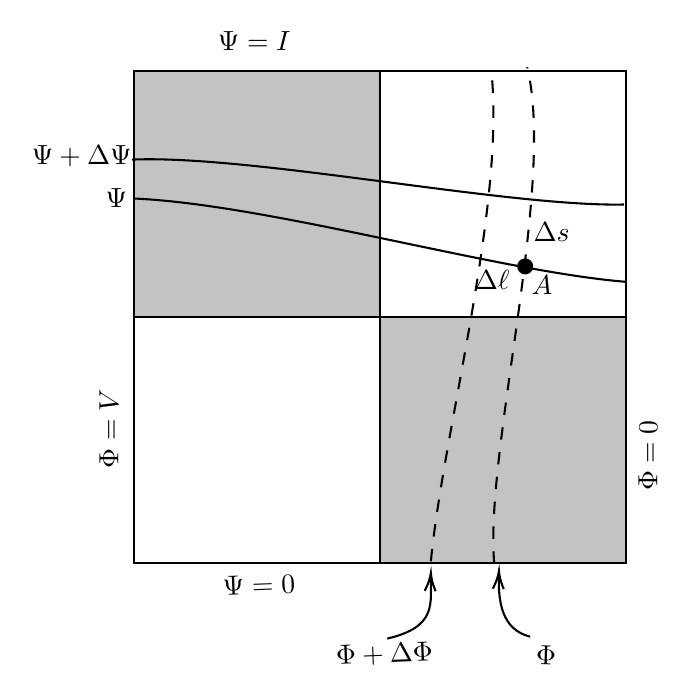
\begin{tikzpicture}[x=0.75pt,y=0.75pt,yscale=-0.8,xscale=0.8]
%uncomment if require: \path (0,493); %set diagram left start at 0, and has height of 493

%Shape: Square [id:dp9280066043832949] 
\draw   (127.75,356.95) -- (127.75,208.8) -- (275.9,208.8) -- (275.9,356.95) -- cycle ;
%Shape: Square [id:dp514561590344355] 
\draw  [fill={rgb, 255:red, 155; green, 155; blue, 155 }  ,fill opacity=0.6 ] (127.75,208.8) -- (127.75,60.65) -- (275.9,60.65) -- (275.9,208.8) -- cycle ;
%Shape: Rectangle [id:dp25055553673842357] 
\draw  [fill={rgb, 255:red, 155; green, 155; blue, 155 }  ,fill opacity=0.6 ] (275.9,356.95) -- (275.9,208.8) -- (424.05,208.8) -- (424.05,356.95) -- cycle ;
%Shape: Rectangle [id:dp3891689331482282] 
\draw   (275.9,208.8) -- (275.9,60.65) -- (424.05,60.65) -- (424.05,208.8) -- cycle ;
%Curve Lines [id:da8672120559593937] 
\draw    (424.35,187.77) .. controls (348.02,181.76) and (209.79,141.19) .. (127.75,137.58) ;
%Curve Lines [id:da13193268906435218] 
\draw    (422.85,141.19) .. controls (352.53,142.69) and (199.27,111.14) .. (126.55,114.14) ;
%Curve Lines [id:da22391912647697598] 
\draw  [dash pattern={on 4.5pt off 4.5pt}]  (306.55,356.05) .. controls (314.07,277.92) and (351.03,142.69) .. (343.13,62.58) ;
%Curve Lines [id:da5306289937649764] 
\draw  [dash pattern={on 4.5pt off 4.5pt}]  (344.72,357.55) .. controls (338.71,289.94) and (381.87,129.24) .. (364.55,58.55) ;
%Curve Lines [id:da14900834515123673] 
\draw    (280.26,402.62) .. controls (310.74,395.48) and (306.26,381.22) .. (306.51,364.84) ;
\draw [shift={(306.55,363.05)}, rotate = 452.22] [color={rgb, 255:red, 0; green, 0; blue, 0 }  ][line width=0.75]    (10.93,-3.29) .. controls (6.95,-1.4) and (3.31,-0.3) .. (0,0) .. controls (3.31,0.3) and (6.95,1.4) .. (10.93,3.29)   ;
%Curve Lines [id:da20565862456805784] 
\draw    (366.35,401.48) .. controls (348.97,397.07) and (347.02,380.12) .. (347.5,363.55) ;
\draw [shift={(347.56,361.75)}, rotate = 452.22] [color={rgb, 255:red, 0; green, 0; blue, 0 }  ][line width=0.75]    (10.93,-3.29) .. controls (6.95,-1.4) and (3.31,-0.3) .. (0,0) .. controls (3.31,0.3) and (6.95,1.4) .. (10.93,3.29)   ;
%Shape: Ellipse [id:dp4968562636978755] 
\draw  [fill={rgb, 255:red, 0; green, 0; blue, 0 }  ,fill opacity=1 ] (363.35,182.66) .. controls (361.02,182.66) and (359.14,180.77) .. (359.14,178.45) .. controls (359.14,176.13) and (361.02,174.24) .. (363.35,174.24) .. controls (365.67,174.24) and (367.55,176.13) .. (367.55,178.45) .. controls (367.55,180.77) and (365.67,182.66) .. (363.35,182.66) -- cycle ;


% Text Node
\draw (179.11,363.54) node [anchor=north west][inner sep=0.75pt]  [rotate=-357.79]  {$\Psi =0$};
% Text Node
\draw (247.29,405.07) node [anchor=north west][inner sep=0.75pt]  [rotate=-357.75]  {$\Phi +\Delta \Phi $};
% Text Node
\draw (368.26,404.93) node [anchor=north west][inner sep=0.75pt]  [rotate=-1.46]  {$\Phi $};
% Text Node
\draw (105.12,302.08) node [anchor=north west][inner sep=0.75pt]  [rotate=-270]  {$\Phi =V$};
% Text Node
\draw (176.37,35.32) node [anchor=north west][inner sep=0.75pt]    {$\Psi =I$};
% Text Node
\draw (429.67,315.59) node [anchor=north west][inner sep=0.75pt]  [rotate=-270]  {$\Phi =0$};
% Text Node
\draw (108.85,129.87) node [anchor=north west][inner sep=0.75pt]    {$\Psi $};
% Text Node
\draw (64.35,103.93) node [anchor=north west][inner sep=0.75pt]    {$\Psi +\Delta \Psi $};
% Text Node
\draw (366.58,150.25) node [anchor=north west][inner sep=0.75pt]    {$\Delta s$};
% Text Node
\draw (331.12,179.08) node [anchor=north west][inner sep=0.75pt]    {$\Delta \ell $};
% Text Node
\draw (365.35,181.85) node [anchor=north west][inner sep=0.75pt]    {$A$};


\end{tikzpicture}
    \end{center}
Một câu hỏi được đặt ra là sau khi quay đĩa, vôn thế và ampe thế đã bị hoán đổi cho nhau và liệu có thể nhân các giá trị vừa tìm được ở trên với một hệ số sao cho kết quả thu được là vôn thế và ampe thế ở mạng mới
\\Chúng ta đặt 
$$\Phi'=\dfrac{I}{V}\Phi~~~~ \text{và} ~~~~ \Phi'=\dfrac{V}{I}\Psi,$$
và đặt các vi phân khoảng cách mới như sau
$$\Delta \ell'=\Delta s ~~~~ \text{và} ~~~~ \Delta s'=\Delta \ell.$$
Các hệ số nhân được chọn sao cho giá trị lớn nhất của $\Phi'$ (giá trị vôn thế mới) là $V$ và $\Psi'$ (giá trị ampe thế mới) là $I$. Nếu các thông số này được dùng để mô tả mạng ban đầu chưa quay thì ta có các mô tả như hình 3, mà ở đây điểm $B$ đã được thay thế cho điểm $A$ bị quay đi. Như đã nói ở trên, vì $B$ và $A$ nằm trên hai ô vuông khác màu nhau nên tích độ dẫn điện của chúng là
$$\sigma_A \sigma_B=\sigma_1 \sigma_2.$$
Tích này luôn không đổi với mọi $A$ do đó cũng là mọi $B$ bất kì mà ta chọn được trên bề mặt mạng.
\begin{center}
    

\tikzset{every picture/.style={line width=0.75pt}} %set default line width to 0.75pt        

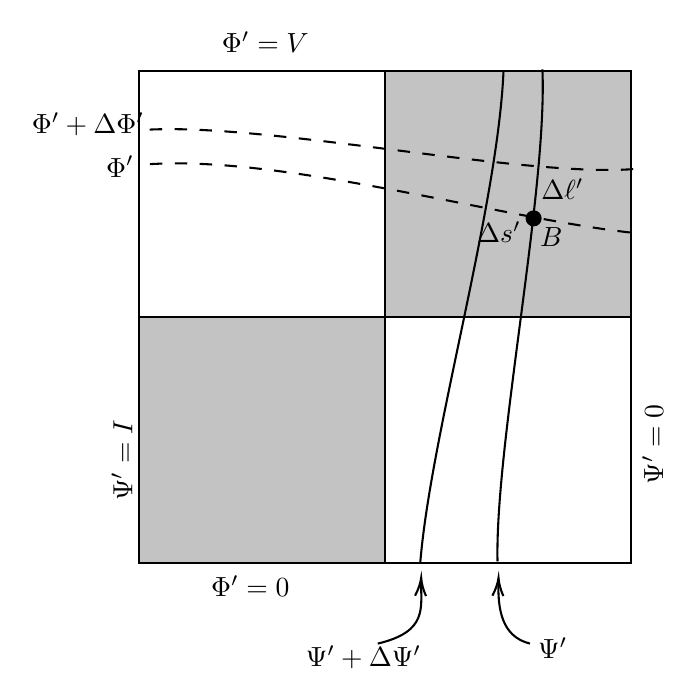
\begin{tikzpicture}[x=0.75pt,y=0.75pt,yscale=-0.8,xscale=0.8]
%uncomment if require: \path (0,493); %set diagram left start at 0, and has height of 493

%Shape: Square [id:dp31479806047094105] 
\draw   (173.81,63.44) -- (321.96,63.44) -- (321.96,211.59) -- (173.81,211.59) -- cycle ;
%Shape: Square [id:dp12949761622436307] 
\draw  [fill={rgb, 255:red, 155; green, 155; blue, 155 }  ,fill opacity=0.6 ] (321.96,63.44) -- (470.11,63.44) -- (470.11,211.59) -- (321.96,211.59) -- cycle ;
%Shape: Rectangle [id:dp29530289497161855] 
\draw  [fill={rgb, 255:red, 155; green, 155; blue, 155 }  ,fill opacity=0.6 ] (173.81,211.59) -- (321.96,211.59) -- (321.96,359.74) -- (173.81,359.74) -- cycle ;
%Shape: Rectangle [id:dp27254309481109895] 
\draw   (321.96,211.59) -- (470.11,211.59) -- (470.11,359.74) -- (321.96,359.74) -- cycle ;
%Curve Lines [id:da3936462898775357] 
\draw    (343,360.04) .. controls (349.01,283.71) and (389.57,145.48) .. (393.18,63.44) ;
%Curve Lines [id:da633404077564983] 
\draw    (389.57,358.54) .. controls (388.07,288.22) and (419.62,134.96) .. (416.62,62.24) ;
%Curve Lines [id:da8011163528814265] 
\draw  [dash pattern={on 4.5pt off 4.5pt}]  (469.24,160.51) .. controls (391.23,151.86) and (256.56,112.95) .. (176.34,119.68) ;
%Curve Lines [id:da9824859596396291] 
\draw  [dash pattern={on 4.5pt off 4.5pt}]  (471.3,122.37) .. controls (403.61,127.4) and (243.6,93) .. (173.6,99) ;
%Curve Lines [id:da7118671539596113] 
\draw    (317.45,408.12) .. controls (347.9,400.87) and (343.37,386.62) .. (343.56,370.24) ;
\draw [shift={(343.6,368.45)}, rotate = 452.01] [color={rgb, 255:red, 0; green, 0; blue, 0 }  ][line width=0.75]    (10.93,-3.29) .. controls (6.95,-1.4) and (3.31,-0.3) .. (0,0) .. controls (3.31,0.3) and (6.95,1.4) .. (10.93,3.29)   ;
%Curve Lines [id:da6417403118429024] 
\draw    (409.11,408.12) .. controls (391.71,403.77) and (389.7,386.83) .. (390.12,370.25) ;
\draw [shift={(390.18,368.45)}, rotate = 452.01] [color={rgb, 255:red, 0; green, 0; blue, 0 }  ][line width=0.75]    (10.93,-3.29) .. controls (6.95,-1.4) and (3.31,-0.3) .. (0,0) .. controls (3.31,0.3) and (6.95,1.4) .. (10.93,3.29)   ;
%Shape: Ellipse [id:dp5170210107145217] 
\draw  [fill={rgb, 255:red, 0; green, 0; blue, 0 }  ,fill opacity=1 ] (407.11,152.04) .. controls (407.11,149.71) and (408.99,147.83) .. (411.31,147.83) .. controls (413.64,147.83) and (415.52,149.71) .. (415.52,152.04) .. controls (415.52,154.36) and (413.64,156.24) .. (411.31,156.24) .. controls (408.99,156.24) and (407.11,154.36) .. (407.11,152.04) -- cycle ;


% Text Node
\draw (474.94,314.07) node [anchor=north west][inner sep=0.75pt]  [rotate=-270]  {$\Psi '=0$};
% Text Node
\draw (107.24,86.66) node [anchor=north west][inner sep=0.75pt]    {$\Phi '+\Delta \Phi '$};
% Text Node
\draw (152.04,112.72) node [anchor=north west][inner sep=0.75pt]    {$\Phi '$};
% Text Node
\draw (221.68,37.81) node [anchor=north west][inner sep=0.75pt]    {$\Phi '=V$};
% Text Node
\draw (155.24,324.06) node [anchor=north west][inner sep=0.75pt]  [rotate=-270]  {$\Psi '=I$};
% Text Node
\draw (215.17,365.36) node [anchor=north west][inner sep=0.75pt]    {$\Phi '=0$};
% Text Node
\draw (412.11,402.52) node [anchor=north west][inner sep=0.75pt]    {$\Psi '$};
% Text Node
\draw (272.23,407.44) node [anchor=north west][inner sep=0.75pt]    {$\Psi '+\Delta \Psi '$};
% Text Node
\draw (375.41,152.16) node [anchor=north west][inner sep=0.75pt]    {$\Delta s'$};
% Text Node
\draw (414.09,126.2) node [anchor=north west][inner sep=0.75pt]    {$\Delta \ell '$};
% Text Node
\draw (413.31,155.44) node [anchor=north west][inner sep=0.75pt]    {$B$};


\end{tikzpicture}
\end{center}
Định luật Ohm được áp dụng bởi vôn thế và ampe thế sau khi quay, ta thu được 
$$t\sigma_B\dfrac{\Delta\Phi'}{\Delta\ell'}=\dfrac{\Delta\Psi'}{\Delta s'}.$$
Sử dụng mối liên hệ giữa các đại lượng trước và sau khi quay như ta đã đặt ở trên, ta thu được biến đổi:
\[t{\sigma _B}\frac{V}{I}\frac{\Delta \Psi}{\Delta s} = t{\sigma _B}\frac{V}{I}.t{\sigma _A}\frac{\Delta \Phi  }{\Delta  \ell} = \frac{I}{V}\frac{\Delta \Phi}{\Delta \ell}.\]
Biểu thức này có thể được đơn giản hóa bằng cách dùng tích độ dẫn điện không đổi và ta thu được giá trị của dòng điện 
\[I = Vt\sqrt {{\sigma _A}{\sigma _B}}  = Vt\sqrt {{\sigma _1}{\sigma _2}}, \]
và đây là kết quả mà chúng ta đã suy đoán ban đầu!!
\\ \textbf{Mở rộng}:
 \begin{itemize}
     \item Tất cả các lập luận ở trên không chỉ đúng với mạng 2x2 mà còn đúng với cả bàn cờ 8x8 bình thường. Một cách tổng quát, cách giải trên có thể được áp dụng với mọi bàn cờ chứa n$\times$n hình vuông miễn sao $n$ phải là số chẵn. Vì nếu $n$ là số lẻ, khi quay bàn cờ $90^\circ$ không hề đổi màu của ô vuông và hơn nữa số ô màu trắng và màu đen là khác nhau nên kết quả không thể chứa $\sigma_1$ và $\sigma_2$ một cách đối xứng.
     \item Sử dụng phương pháp tính số, ta có thể tìm và vẽ được các đường dòng và các đường đẳng thế của bất kì bàn cờ nào, như được vẽ ở hình dưới 

    \begin{center}
        \includegraphics[scale=0.6]{Anh/Nam2.pdf}
    \end{center}
     Vì điều kiện biên, các đường dòng và đường sức từ bị gấp khúc khi gặp các bề mặt phân cách, tương tự như sự truyền ánh sáng.
  \end{itemize}
\end{loigiai}

